\documentclass[12pt]{article}%
\usepackage[a4paper, top=1in, bottom=1in, left=0.9in, right=0.9in]{geometry}
\usepackage{amsmath,amsthm}
\usepackage{amssymb}
\usepackage{amsfonts}
\usepackage{enumerate}
\usepackage{rotating}
\usepackage{setspace}
\usepackage{footmisc}
\usepackage{graphicx}
\usepackage{caption}
\usepackage{subcaption}
\usepackage{float}
\usepackage{natbib}
\usepackage{bm}
\usepackage{color}
\usepackage{placeins}
\usepackage{amsmath}
\usepackage{hyperref}
\hypersetup{colorlinks=true,citecolor=blue,linkcolor=red,filecolor=green,urlcolor=red}
\setcounter{MaxMatrixCols}{30}
\allowdisplaybreaks[1]
\overfullrule=0mm
\usepackage{todonotes}

\usepackage{pgfplots}
\pgfplotsset{compat=1.17}
\usepgfplotslibrary{fillbetween}
\usetikzlibrary{patterns,arrows.meta}
\usepackage{subcaption}
\definecolor{resteal}{RGB}{29,158,117}
\definecolor{floororange}{RGB}{216,90,48}
\definecolor{pregray}{RGB}{136,135,128}
\definecolor{excessamber}{RGB}{186,117,23}

\usepackage{array}       
\usepackage{tabularx}
    %\setlength{\extrarowheight}{5pt}
\usepackage[flushleft]{threeparttable}
\usepackage{booktabs}
\usepackage{dcolumn} 
  \newcolumntype{d}[1]{D{.}{.}{#1}}  
\usepackage{multirow}
\newcolumntype{s}{>{\hsize=.2\hsize}X}
\newcommand\Tstrut{\rule{0pt}{2.6ex}}         % = `top' strut
\newcommand\Bstrut{\rule[-0.9ex]{0pt}{0pt}}   % = `bottom' strut

% to change the symbols associated with the authors
%\makeatletter
% *, 1, 2, ...
%\renewcommand*{\@fnsymbol}[1]{\ifcase#1\or*\else\@alph{\numexpr#1-1\relax}\fi}
%\renewcommand*{\@fnsymbol}[1]{\@alph{\numexpr#1}}
%\makeatother

%\onehalfspacing


\def\citetpos#1{\citeauthor{#1}'s (\citeyear{#1})}
\def\citeauthorpos#1{\citeauthor{#1}'s}
%\defcitealias{FRWZ2015}{FRWZ}  %\citetalias{FRWZ2015} %\citepalias{FRWZ2015}


\newcommand{\vect}[1]{\bm{#1}}
%\newcommand{\vect}[1]{\boldsymbol{\mathbf{#1}}}

\newtheorem{result}{Result}
\newtheorem*{result_nonumb}{Result}
\newtheorem{proposition}{Proposition}
\newtheorem{corollary}{Corollary}
\theoremstyle{remark}
\newtheorem{rem}{Remark}
\defcitealias{GordonKrenn2010}{Gordon-Krenn (2010)}



%\title{Which Fiscal Spending Category Is the Most Inflationary?
%\title{Dissecting Fiscal Inflation}
\title{The Inflationary Footprint of Fiscal Policy:\\
Evidence from Disaggregated U.S. Spending\thanks{Florio acknowledges financial support from the Italian Ministry of Education, Universities, and Research (PRIN 2022, grant 2022A9PAT3). The views expressed in this presentation are those of the authors and do not necessarily reflect the views of the De Nederlandsche Bank (DNB) or any other person associated with the Eurosystem. Any errors and omissions are the sole responsibility of the authors.}}
%F.

\author{%
\makebox[\textwidth][c]{%
  \begin{tabular}{cc}
    Guido Ascari\thanks{Corresponding author: Guido Ascari, Department of Economics and Management, University of Pavia, Via San Felice 5, 27100 Pavia, Italy, E-mail: guido.ascari@unipv.it, and De Nederlandsche Bank, Frederiksplein 61, 1017XL Amsterdam, The Netherlands, E-mail: g.ascari@dnb.nl.}
    & Anna Florio\thanks{Department of Management, Economics and Industrial Engineering, Politecnico di Milano, via Lambruschini 4/B, 20156 Milan, Italy. E-mail: anna.florio@polimi.it.} \\
    \normalsize{\textit{University of Pavia,}}
	& \normalsize{\textit{Politecnico di Milano}} \\
    \normalsize{\textit{De Nederlandsche Bank, and CEPR}}  \\[2ex]
    Alessandro Gobbi\thanks{Department of Environmental Science and Policy, University of Milan, via Celoria, 2, 20133 Milan, Italy. E-mail: alessandro.gobbi@unimi.it.}
    & Leonardo Melosi\thanks{Department of Economics, European University Institute, via delle Fontanelle 18, 50014 Fiesole (FI), Italy. E-mail: leonardo.melosi@eui.eu.} \\
    \normalsize{\textit{University of Milan}}
 &\normalsize{\textit{European University Institute and CEPR}}
% \\
%    & \normalsize{\textit{and CEPR}} \\
  \end{tabular}%
}}

\date{\vspace{2ex} March 2026\vspace{-4ex}}
\begin{document}
\maketitle


%\begin{center}
 %   \Large{PRELIMINARY, PLEASE DO NOT CIRCULATE}
%\end{center}
%\vspace{-3ex}
\begin{abstract}  %92 words
\singlespacing

\vspace{-3ex}


Under the Fiscal Theory of the Price Level (FTPL), wealth effects arise when government spending is fiscally unfunded—that is, not backed by future fiscal adjustment. Under U.S. statutory budget rules, Medicare and Medicaid are granted priority access to general revenues and thus enjoy stronger fiscal backing; correspondingly, their expansions generate negligible wealth effects in the data. By contrast, defense spending undertaken when discretionary fiscal space is constrained or during major wars is more likely to be unfunded and, in the data, generates wealth effects and inflation. An asymmetry in Social Security's trust-fund design implies that pre-1974 benefits were actuarially funded but fiscally unfunded, whereas an actuarial deficit after 1974 implied fiscal backing. Accordingly, only pre-1974 Social Security expansions generated wealth effects and inflation.

%\vspace{16pt}


\medskip
\noindent\textit{Keywords:} Fiscal backing, wealth effects, Ricardianity, Monetary and fiscal interactions, anticipated shocks, fiscal shocks.

\smallskip
\noindent\textit{JEL classification:} E52, E62, E63.
\end{abstract}

\setcounter{page}{0}
\thispagestyle{empty} 
\newpage
%\listoftodos
\doublespace
\section{Introduction}

The fiscal theory of the price level holds that fiscally unfunded government spending raises households' perceived wealth, boosting demand and inflation until the real value of public debt is consistent with expected future primary surpluses. In recent years, economic research has made important progress in showing that the fiscal theory of the price level provides a coherent framework for understanding macroeconomic dynamics across countries and time \citep{Bianchiillut, BM2017, LeeperTraumWalker:2017,EusepiPreston2018,Cochranebook,BFM2023,JacobsonLeeperPreston2024,Barro_Bianchi25}. 
Nonetheless, whether government spending is fiscally funded or unfunded hinges on the government’s willingness to adjust future primary surpluses to repay the public debt issued to finance the increase in spending.
This willingness---commonly referred to as fiscal backing---must be assessed intertemporally and is inherently forward-looking, which makes it difficult to observe directly. Given this challenge, most empirical work evaluates fiscal backing \textit{ex post}, by examining the joint responses of monetary and fiscal variables to unexpected innovations in government spending.

This paper introduces a novel ex-ante strategy to assess whether fiscal shocks are fiscally funded or unfunded. Our approach exploits program-specific funding mechanisms established under U.S. law to measure fiscal backing across major categories of U.S. government spending---Social Security, Medicaid and Medicare and national defense. We leverage cross-category heterogeneity in funding regimes to identify whether spending expansions require the government to eventually adjust taxes, cut other spending, or draw on future tax revenues, or instead allow expenditures to be financed through debt issuance without a statutory fiscal backstop. Only in the latter case does the fiscal theory of the price level predict positive effects on output and inflation --i.e., non-Ricardian effects-- following the announcement of an expansion in government spending. The proposed framework provides a new and more direct way to evaluate the fiscal theory of the price level empirically. %Rather than inferring fiscal backing from 

Our analysis highlights a fundamental distinction between discretionary and mandatory spending in their financing structures. Discretionary spending---such as National security---is subject to the congressional appropriations process and lacks fiscal backing when available fiscal resources are scarce, typically because mandatory spending absorbs a large share of available fiscal resources. Mandatory spending, by contrast, operates under fundamentally different financing rules and is largely insulated from short-run budgetary constraints.

This distinction matters because the fiscal funding of a spending program depends on whether its financing rules generate credible expectations of future adjustment. A key implication is what we call the \textit{paradox of solvency}. Programs financed through dedicated trust funds are subject to an asymmetric adjustment rule: corrective action—higher contributions or lower benefits—is triggered when the trust fund is projected to become insolvent, whereas no mechanism returns excess resources when it is projected to remain solvent. Hence, a trust-fund program is fiscally funded precisely when it is actuarially unfunded, and fiscally unfunded when it is actuarially funded. We formalize this mechanism in a stylized general equilibrium model and use it to organize the empirical analysis: the model predicts which spending expansions should generate wealth effects and inflation, and the data test these predictions across programs.

Social Security provides the sharpest test of this mechanism, as it is the only major spending program whose actuarial position changed sign over our sample. It is financed through dedicated trust funds—the Old-Age and Survivors Insurance and Disability Insurance (OASI/DI) funds—which are legally segregated from general federal revenues. When these trust funds are projected to become dynamically insolvent, as was the case after 1974, existing law requires either legislative action to adjust benefits or payroll taxes; absent such action, benefits would be reduced mechanically to the level of incoming payroll tax revenues, with across-the-board cuts administered by the Social Security Administration. In practice, however, Congress has never allowed such benefit reductions to take effect, most likely because they would be politically untenable. Instead, it has repeatedly intervened to restore solvency through adjustments to benefits and payroll taxation, most notably through the 1977 amendments, the Social Security Amendments of 1983, the expansion of benefit taxation in 1993, the 1994 DI Reallocation, and repeated adjustments to the payroll tax base through increases in the taxable earnings cap.

Taken together, this recurring pattern of legislative intervention and statutory backstops constitutes a strong and credible commitment to ensure that Social Security spending remains fiscally backed. Importantly, this commitment operates within a strict legal framework: the OASI/DI trust funds are separate from general fiscal revenues, and neither the Social Security Administration nor the U.S. Treasury is authorized to borrow to stabilize them. As a result, fiscal backing for Social Security must ultimately be delivered through explicit legislative action, reinforcing the perception that these spending commitments will be honored through either future fiscal adjustments or spending cuts.
Prior to 1974, however, the prevailing view was that the Social Security system was solvent and was projected to remain so indefinitely (Board of Trustees, 1973; U.S. General Accounting Office, 1974).\footnote{Prior to 1974, official long-run projections suggested only a modest actuarial imbalance in the Social Security system, reinforcing the prevailing view that the program was broadly solvent under then-prevailing demographic and economic assumptions \citep{SSA1973Trustees,GAO1974SSFinancing}. This perception changed sharply with the release of the 1974 Trustees Report (House Document No.~93--313), which documented a substantial deterioration in long-run finances---amounting to nearly 3 percent of taxable payroll---driven primarily by revised population projections and the interaction of high inflation with the benefit indexation rules enacted in 1972 \citep{SSA1974Trustees}. In response to the severity of this reassessment, the Senate Committee on Finance commissioned an independent expert review, whose January 1975 report, chaired by George C. Hsiao, confirmed and in some respects worsened the Trustees' diagnosis, concluding that earlier projections had been overly optimistic and that significant policy adjustments would be required to restore long-run balance \citep{Hsiao1975Report}.} 
During this period, the OASI and DI trust funds generated persistent surpluses, which by statute were invested in special, nonmarketable Treasury securities. The proceeds were transferred to the U.S. Treasury’s General Fund, where they were commingled with general federal revenues and used to finance other government expenditures, thereby reducing the Treasury’s need to borrow from the public in the short run.
Under the prevailing belief that Social Security would generate surpluses indefinitely, no explicit provision was made to accumulate resources for the eventual repayment of these intragovernmental obligations. Moreover, because the proceeds were commingled with general federal revenues and no explicit mechanism was established to fund their repayment, it was unclear how these intragovernmental Treasury obligations would be honored should the trust funds later run deficits.
From the perspective of the Fiscal Theory of the Price Level, pre-1974 Social Security spending was therefore fiscally unfunded precisely because it was expected to be actuarially funded. A funding system centered on trust funds provides credible fiscal backing only when the system is perceived to be dynamically insolvent—either inducing congressional intervention or mechanically triggering automatic benefit reductions. By contrast, when the system is expected to remain solvent over an extended horizon and to accumulate rising reserves, the trust-fund framework offers no mechanism for reallocating or returning the excess resources being accumulated. What matters for the price level is not whether the program runs surpluses or deficits, but whether changes in its balance are expected to be offset by future fiscal adjustment. Hence, although pre-1974 Social Security was expected to be dynamically solvent, the asymmetry in its trust-fund design left its expansions fiscally unfunded; the same mechanism implies fiscal (though not actuarial) funding once trust-fund insolvency became anticipated after 1974.
Accordingly, announcements of Social Security expansions prior to 1974 were inflationary: by reducing the surpluses the system was expected to accumulate indefinitely, they lowered the present value of primary surpluses without triggering any offsetting adjustment, thereby generating positive wealth effects. By contrast, Social Security was perceived as actuarially insolvent after 1974 and thus entered a regime of full fiscal backing. In this context, announcements of program expansions no longer generated wealth effects or inflationary pressures, as they gave rise to expectations of future tax increases or benefit offsets.

Medicare and Medicaid, by contrast, never entered the solvency region and thus provide a natural counterpart to Social Security. A large share of Medicare ---Medicare Part B and D--- and Medicaid are fiscally backed by statute, as U.S. budgetary law grants these programs priority access to general tax revenues. Medicare Parts B and D are financed through the Supplementary Medical Insurance (SMI) trust fund, which receives automatic transfers from general revenues sufficient to cover projected expenditures. In addition, beneficiary premiums are reset annually to finance a fixed share of program costs (roughly one-quarter), with income-related premium surcharges further reinforcing revenue adequacy. Medicaid spending is similarly fiscally backed, as the federal government is legally obligated to finance its share of eligible outlays through the Federal Medical Assistance Percentage (FMAP), with federal transfers adjusting automatically to program costs. Through the lens of our framework, these programs represent a limiting case in which the correction is automatic and occurs every period.
Medicare Part A, which covers hospital insurance, is financed in a manner analogous to Social Security, in that it relies on a dedicated trust fund—the Hospital Insurance (HI) Trust Fund—whose financing needs cannot be met through general federal revenues. Unlike Social Security, however, the HI Trust Fund has been repeatedly projected to face insolvency since its inception.\footnote{See, for example, Congressional Research Service, \emph{Medicare’s Insolvency Projections}, updated October 25, 2021, available at \href{https://www.congress.gov/crs_external_products/RS/HTML/RS20946.web.html}{Link to report}.} Yet, like Social Security, it has never actually become insolvent: projected insolvency dates have been postponed on multiple occasions through legislative interventions. In the early years of the program, for example, payroll tax rates were periodically adjusted to maintain the financial adequacy of the HI Trust Fund.\footnote{In the early years of the program, for example, Congress repeatedly adjusted the HI payroll tax rate and tax base—most notably through the Social Security Amendments of 1972 and the Social Security Amendments of 1977---to maintain the financial adequacy of the HI Trust Fund. More recently, revenue increases and spending adjustments under the Affordable Care Act substantially extended the projected exhaustion date. This pattern reflects a financing regime in which Medicare Part A is sustained through discretionary policy adjustments rather than adherence to a stable, actuarially balanced funding rule.} 
Although the HI Trust Fund is required to remain financially balanced, this balance has been maintained through intermittent legislative interventions in response to projected shortfalls, rather than through an ex-ante commitment to long-run actuarial balance as in Social Security. These repeated interventions have been politically acceptable because projected solvency horizons depend on many unpredictable factors, including highly volatile health care cost drivers (e.g., provider prices and utilization) and a weak linkage between contributions and benefits. In addition, Medicare does not operate under the same earned-benefit norm that disciplines Social Security, where benefits are closely tied to lifetime payroll contributions and are widely perceived as entitlements earned through prior work rather than as discretionary transfers.
Medicare Part A has therefore always been in the region where the paradox of solvency predicts fiscal backing. Accordingly, despite differences in statutory financing rules, we do not distinguish it from the other components of Medicare, which, as argued above, are likewise fiscally backed under existing statutory arrangements.

Discretionary spending is the other side of the same principle. National defense has no dedicated account and no automatic access to general revenues: its fiscal backing depends on the resources left once mandatory programs, which enjoy priority, have been financed. By absorbing fiscal space, Medicare and Medicaid tighten this constraint. We show that when it binds, increases in defense spending generate non-Ricardian effects and upward pressure on inflation. These effects are also present during periods in which the U.S. government financed the three most expensive wars of the past 75 years—a phenomenon we label warflation.

We test these predictions by examining the responses of output, inflation, the interest rate–growth differential, and public debt to news about increases in Social Security, Medicare and Medicaid and National defense spending. 

Building on the shock construction methodology of \cite{ForniGambetti2016}, we depart from standard measures of aggregate government spending by computing distinct series of anticipated shocks for each spending category directly from U.S. Federal Budget expenditure forecasts. We then study their effects using state-dependent local projections, where the state variable reflects the financing rules of each category: the long-term actuarial balance of the relevant trust funds for Social Security and Medicare, and the residual fiscal space available after mandatory outlays for national defense. These forward-looking measures capture the degree of fiscal strain and serve as a proxy for fiscal backing.

\textbf{Literature Review.} This paper is related to four different streams of literature. 
The first encompasses the broad research on monetary-fiscal policy interactions, with a particular focus on the Fiscal Theory of the Price Level (FTPL). Foundational theoretical contributions include the seminal works by \cite{sargentWallace1981}, \cite{Leeper1991}, \cite{Sims1994} and \cite{Woodford2001}, which formalize the conditions under which fiscal policy can be a key driver of the price level. More recent studies embed FTPL mechanisms in structural models to explore their implications for macroeconomic dynamics and policy design (see, among others, \cite{Cochranebook} and \cite{leeperleithcampbell2016understanding}).
Building on this framework, a growing number of empirical studies investigate the presence of different monetary-fiscal policy regimes in U.S. data \citep[see, among the others,][]{Bianchi2012,Bianchiillut,AscariFlorioGobbi2020, BM2014, JacobsonLeeperPreston2024}.  


The second stream of literature deals with fiscal foresight and the identification of fiscal policy shocks. This literature examines the impact on the economy of fiscal policy in VAR models \citep[e.g., see][]{ BP,Ramey2011,AuGoro2012,ForniGambetti2016,RameyShapiro,MERTENS2011,MertensRavn2012,BenZeev2017,Fisher} and stresses the importance of accurately distinguishing between anticipated and unanticipated government shocks. Legislative and implementation lags imply that private agents can adjust their behavior during the time between the announcement of a fiscal measure and its actuation. In fact, those who analyze the effects of an anticipated increase in taxes \citep[see][]{MertensRavn2012,MERTENS2011} find that the production increases during the anticipation period and, as happens for unanticipated shocks, decreases once the tax increase is implemented. \cite{Ramey2011}, who analyses the effects of an anticipated government spending shock, finds that such a shock increases output but decreases consumption. 

A relevant paper for our analysis is \cite{ASCARI20231}. They extend the results by \citet{Beck}, who study unanticipated changes in government expenditures under a backed monetary regime and an unbacked fiscal regime, to consider anticipated public spending shocks. 
Theoretically, they show that fiscal foresight leads anticipated government spending shocks to have very different effects if one considers a monetary rather than a fiscal regime. In the monetary regime, increases in government expenditure are assumed to be fiscally backed. Following an anticipated spending shock, output, consumption, investment, and inflation decrease while real interest rates and debt increase. These variables show an opposite reaction in the fiscal regime, under unbacked fiscal expansions, as consumption increases through the expectation of positive wealth effects.
Anticipated shocks can thus provide a potential identification mechanism in the data to distinguish these two regimes. They thus look at two sample periods that have been identified in the literature as a monetary and a fiscal regime and find that anticipated government spending shocks have very different effects during the anticipation period, as theory would predict: in the monetary regime they are contractionary;
%, i.e. output and consumption decrease
in the fiscal regime they are expansionary. 

The third stream of literature is the one on the state dependence of spending multipliers \citep[see][]{AuGoro2012, RameyZuba2018, Caggianoetal2015EJ}. Unlike these studies, however, our focus is not on fiscal multipliers per se. Rather, we are interested in the broader macroeconomic consequences of spending shocks, following the tradition of research inspired by the FTPL, such as \cite{LeeperTraumWalker:2017}, who emphasizes the central role of the policy regime in determining the size and sign of fiscal multipliers. 

A fourth and relatively recent strand of the literature emphasizes the heterogeneity of public expenditure. \cite{coxetal_24}, for example, look at government spending not as a single large transaction, “one big G”, but as the aggregation of numerous smaller transactions, examining federal government procurement contracts through this lens. While we draw inspiration from their granular perspective, our approach is broader in scope. Rather than focusing on a specific subset of spending, we consider a broader set of government expenditures, disaggregated in a manner consistent with how U.S. lawmakers structure the federal budget. This approach allows us to capture different dimensions of fiscal heterogeneity and offers a complementary angle to studies focused solely on procurement spending.


The remainder of the paper is structured as follows. Section \ref{sec: data} describes the institutional features underlying each spending category and the evolution of actuarial projections of trust fund solvency. Section 3 develops a stylized general equilibrium model that rationalizes the paradox of solvency and derives its empirical predictions. Section 4 presents the methodology used to construct our new measure of anticipated, disaggregated spending shocks, and the empirical results for Social Security, Medicare and Medicaid, and National Defense. Section 5 concludes.


\section{Data and Institutional Background\label{sec: data}}\label{sec:background}
\subsection{Federal Spending Categories and Composition} 
Rather than considering aggregate government expenditures, we disaggregate them according to the predominant type of spending: mandatory or discretionary. Mandatory spending refers to expenditures that are required by law and are generally not subject to annual review by Congress. It comprises entitlement programs that are difficult to modify or reduce, as their funding is set by eligibility criteria rather than through the annual appropriations process. Examples include Social Security, Medicare, and Medicaid, which offer guaranteed benefits to eligible individuals and are financed either through dedicated payroll taxes (Social Security and Medicare Part A) or through general revenues (Medicare Parts B and D, and Medicaid).\footnote{A few mandatory programs, for example, veterans' disability compensation and pensions and Medicaid, are also funded through appropriation acts. While pure mandatory programs receive automatic funding, these \textit{appropriated mandatory programs} require funds to be approved through an annual budget process, even though the provision of benefits remains mandatory.} Discretionary spending, on the other hand, encompasses expenditures that Congress must review and approve annually through the appropriations process. This category covers a wide range of government programs, including National Defense (which constitutes about half of the total) and non-defense spending such as education, infrastructure, and many federal agency budgets. Congress decides the specific funding levels for each program within this category every fiscal year, and these levels can be adjusted or reduced according to the policy priorities and available funds. In 2023, health care programs, primarily Medicare and Medicaid, constituted around 28\% of the total budget. The other large category of mandatory spending is Social Security, which received about 23\% of the federal budget. Defense spending, part of discretionary spending, received about 13-14\% of the budget. 
 

\begin{figure}[t!]
    \centering
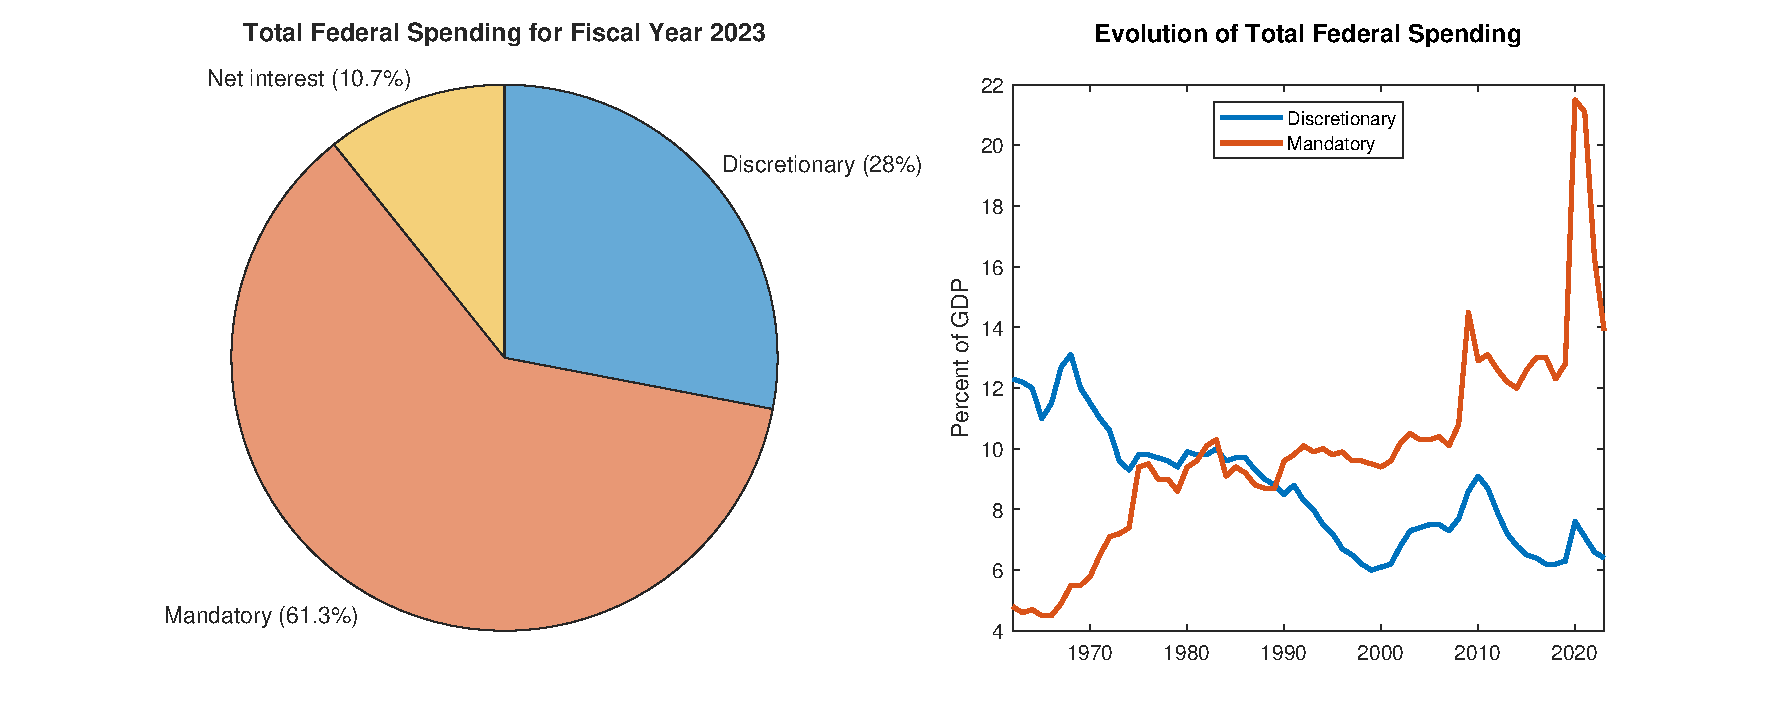
\includegraphics[width=\textwidth]{figures and tables/pie_manda_discr.pdf}
    \caption{\textbf{Mandatory and discretionary spending.} 
    \\[0.5ex]
    \small
    Left panel: composition of total federal spending in Fiscal Year 2023, highlighting the shares of mandatory, discretionary, and net interest spending.
    Right panel: evolution of yearly mandatory and discretionary spending as a share of GDP from 1962 to 2023.
        }
    \label{fig:pie_manda_discr}
\end{figure}


The left panel of Figure \ref{fig:pie_manda_discr} shows the total federal spending data for Fiscal Year 2023. Mandatory spending is more than double the discretionary spending. This has not always been the case: the right panel
%Figure \ref{fig:sharemandiscrtime} 
shows how mandatory and discretionary spending have evolved since the 1960s. Note that, before the 1990s, mandatory spending was lower than discretionary spending.


\begin{figure}[t!]
    \centering
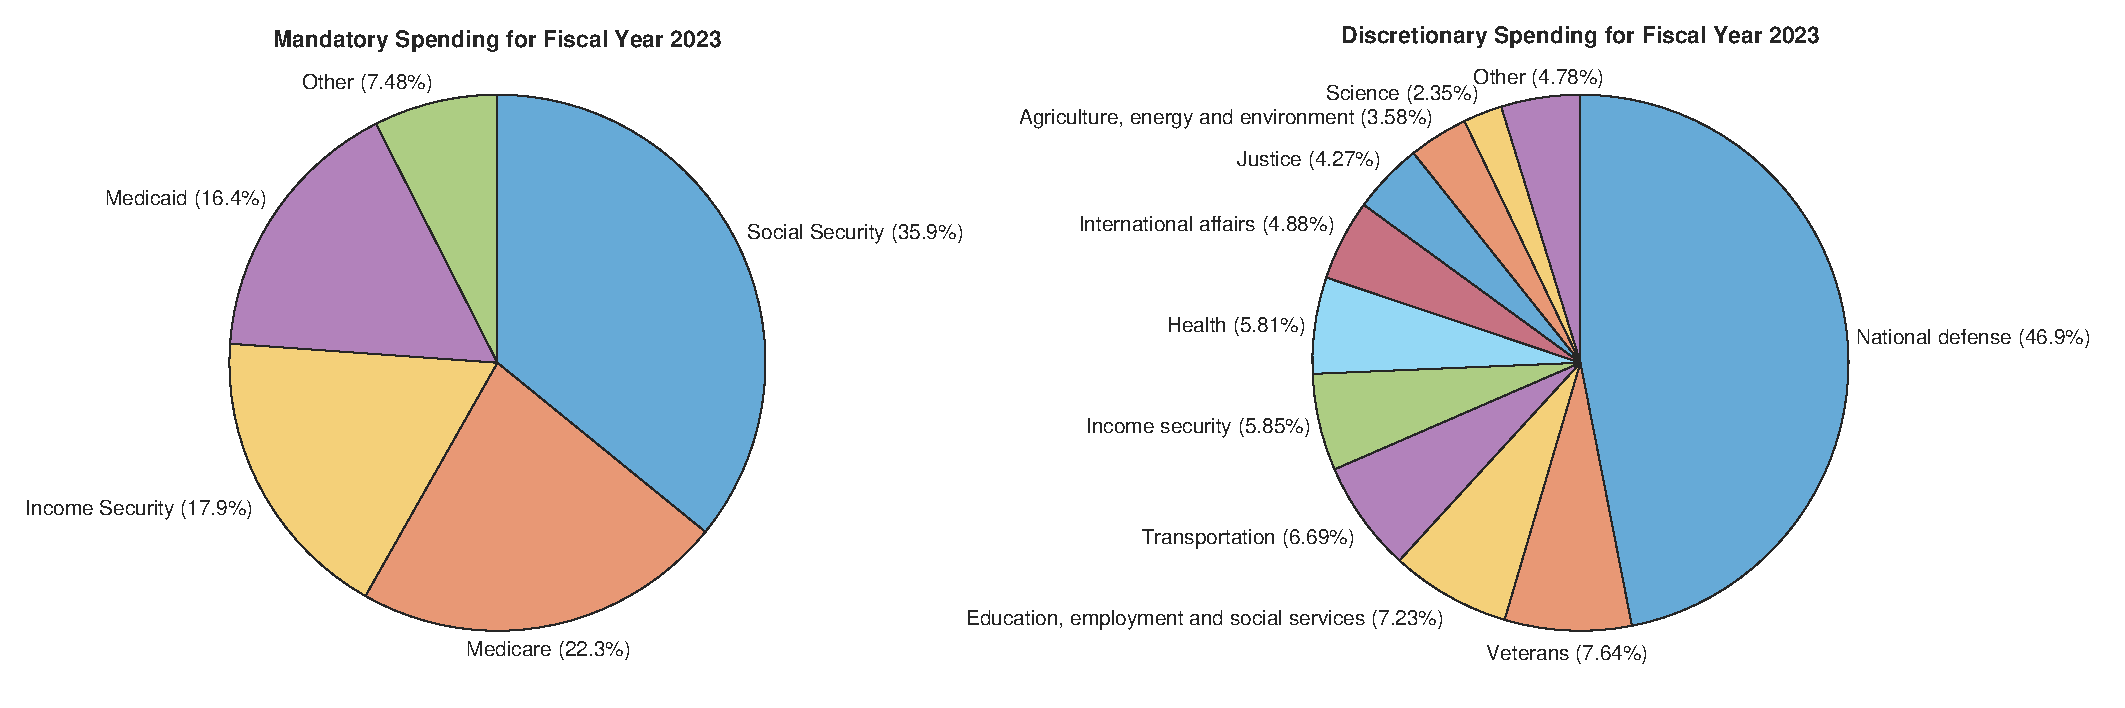
\includegraphics[width=\textwidth]{figures and tables/pie_decomp.pdf}
    \caption{\textbf{Composition of mandatory and discretionary spending in Fiscal Year 2023}.
    \\[0.5ex]
    \small
    Left panel: breakdown of mandatory spending. 
    Right panel: breakdown of discretionary spending. Mandatory spending is largely driven by Social Security, Medicare, and income security programs, while discretionary spending is dominated by national defense.}
    \label{fig:pie_decomp.pdf}
\end{figure}

Figure \ref{fig:pie_decomp.pdf} shows the composition of mandatory and discretionary spending in 2023, respectively.
Among the mandatory spending categories, Social Security (SS) has the largest share at 36\%, followed by Medicare and Medicaid (MM) at 22.3\% and 16.4\%, respectively. In contrast, slightly half of discretionary spending is allocated to National Defense (ND) expenditures, with the remainder going towards non-defense spending (education, transportation, environmental programs, and R\&D).%
\footnote{As a major component of mandatory spending, Medicare comprises four distinct parts—A through D—each covering different health services. See Appendix \ref{app:sec:suppl} for a description of the components of mandatory and discretionary spending, including Medicare Parts A–D, and for figures showing their evolution in levels and growth rates since the 1970s.}
%Since the 1970s, trends in defense spending as a share of GDP have been larger than non-defense spending in the discretionary budget authority.\footnote{See Appendix \ref{app:sec:suppl} for figures showing the components of mandatory and discretionary spending, both in levels and growth rates, since the 1970s.} 
As discussed below, these categories differ not only in size but in the rules that govern their financing, which determine the degree of fiscal backing of each.

\subsection{Institutional Financing Rules and Fiscal Backing}\label{sec:financing} 

To interpret our results, it is essential to clarify how major U.S. federal spending programs are financed and how their institutional design shapes fiscal spillovers across the budget. Two financing regimes coexist: programs automatically backed by general revenues, and programs whose trust funds impose binding solvency constraints.
\paragraph{General-revenue backing.} Medicare Supplementary Medical Insurance (SMI), which covers Parts B and D, is formally organized as a trust fund, but is financed roughly one quarter by beneficiary premiums and three quarters by transfers from general revenues, both adjusted automatically each year to match projected expenditures. SMI therefore cannot experience a solvency crisis in the legal sense: when costs rise or revenues fall, additional general revenues are transferred without requiring new legislation or benefit reductions. Medicaid shares this feature despite not having a trust fund: it is an open-ended entitlement financed through federal matching payments to states and is not subject to an annual appropriations cap. Neither SMI nor Medicaid can “run out of money”: higher spending mechanically translates into higher claims on general revenues.
\paragraph{Trust-fund constraints.} The Old-Age and Survivors Insurance (OASI) and Disability Insurance (DI) trust funds of Social Security, together with the Medicare Hospital Insurance (HI) trust fund, are instead legally binding financing mechanisms. They are financed primarily by dedicated payroll taxes and have no authority to issue debt, no routine access to general revenues, and no automatic Treasury backstop. By law, surpluses are invested in special-issue, nonmarketable Treasury securities, and the corresponding cash is transferred to the Treasury’s General Fund. There it is commingled with general revenues and used to finance other expenditures, reducing the government’s need to borrow from the public. When trust funds run cash deficits, these securities must be redeemed, requiring higher taxes, lower spending, or new public debt. If balances are exhausted, current law prohibits benefit payments in excess of incoming revenues, triggering automatic benefit reductions absent congressional action.
\paragraph{The asymmetry of trust-fund adjustment.} A key feature of this system is the asymmetric nature of its adjustment mechanism. Payroll taxes and benefits are not continuously adjusted to trust-fund balances. When trust funds are solvent and projected exhaustion is distant, no corrective action is required and none is triggered; in particular, no mechanism returns excess reserves. When insolvency becomes salient, by contrast, the institutional framework forces corrective measures sufficient to restore solvency. Historically, approaching depletion of the Social Security and HI trust funds has prompted increases in payroll tax rates, changes in benefit formulas, or adjustments to eligibility rules. Fiscal correction is therefore contingent on projected insolvency rather than on contemporaneous budgetary imbalances.\footnote{As noted in the 1969 Trustees Report, ``in the case of a surplus, the excess contributions actually earn interest, while a deficit grows because of the absence of the annual interest that would have been earned if the contributions required for balance had been paid'' \citep[p.~38]{Trustees1969}.} This asymmetry is the institutional basis of the paradox of solvency, which we formalize in Section \ref{sec:model}.
\paragraph{A pecking order of federal revenues.} Taken together, these features imply a clear pecking order. SMI and Medicaid have a first claim on general revenues; OASI, DI, and HI are constrained by trust-fund solvency; discretionary spending, including national defense, absorbs the residual. As open-ended mandatory programs expand and fiscal space narrows, the financing of discretionary spending relies increasingly on borrowing, potentially giving rise to non-Ricardian outcomes.




\subsection{Actuarial Soundness and Fiscal space} \label{sec:actuarial_soundeness}

The financing rules above imply that the fiscal backing of each spending category depends on a forward-looking measure of fiscal strain: the projected actuarial balance for trust-fund programs, and the residual fiscal space for discretionary spending. We now document how these measures evolved over our sample.
\paragraph{Social Security.} Until the mid-1970s, Social Security was widely viewed as actuarially sound and expected to generate persistent long-run surpluses under current law. Trustees Reports of the late 1960s and early 1970s presented actuarial balances clustered around zero or mildly positive. Under the 1967 Amendments, scheduled payroll tax rates exceeded long-run cost rates, and the system was projected to accumulate substantial trust-fund balances. Favorable demographic and macroeconomic conditions—high fertility, rapid real wage growth, and strong employment—reinforced the perception that Social Security was “overfinanced”,\footnote{\citealp[p.~37]{Trustees1969}} contributing to repeated benefit expansions that culminated in the large benefit increase of 1972.
This regime changed abruptly in 1974. The 1974 Trustees Report replaced near-zero actuarial balances with a deficit of nearly 3 percent of taxable payroll. The deterioration was driven by lower projected fertility, faster improvements in longevity, slower real wage growth and, critically, the interaction of high inflation with the “double indexing” error in the 1972 benefit formula. The consultant panel commissioned by Congress (Hsiao et al., 1975) confirmed that the deterioration reflected structural flaws rather than temporary deviations. From then on, trust-fund exhaustion dates became central to official reporting, and Social Security came to be viewed as requiring periodic legislative intervention to restore solvency, as in the 1977 and 1983 reforms. 
\begin{figure}[t!]
    \centering
    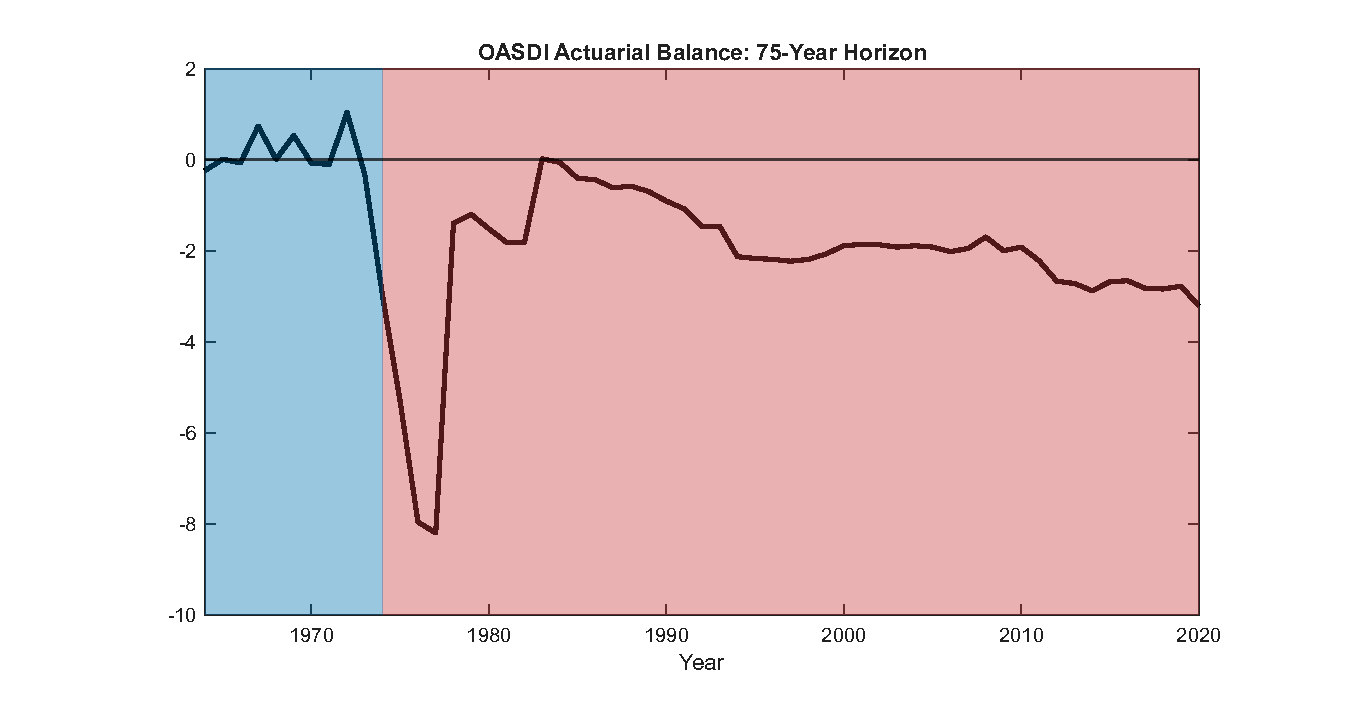
\includegraphics[trim=20mm 00mm 20mm 00mm, clip, scale=0.40]{figures and tables/state_OASDI_actuarial_75y.pdf}
    %\includegraphics[trim=20mm 00mm 20mm 00mm, clip, scale=0.40]{figures and tables/state_OASDI.pdf}
\caption{\textbf{Actuarial fiscal position of Social Security (OASDI).}
\\[0.5ex]
\small
Evolution of the 75-year actuarial balance for the combined Old-Age and Survivors Insurance (OASI) and Disability Insurance (DI) trust funds (OASDI), based on data from the Trustees Reports. Shaded areas distinguish periods in which the system is perceived as actuarially funded (blue areas), when the projected balance is positive and no fiscal adjustment is expected, from periods in which it is actuarially unfunded (red areas), when projected deficits give rise to expectations of future fiscal adjustment.}
 \label{fig:state_OASDI_actuarial_75y}
\end{figure}
   
Figure \ref{fig:state_OASDI_actuarial_75y} reports the 75-year OASDI actuarial balance, which is positive from 1968 to 1973 and persistently negative thereafter. Appendix \ref{app:sec:supplem} documents the Trustees Reports from 1969 to 1976 in detail.

\paragraph{Medicare Hospital Insurance.} HI presents a contrasting case. From its inception, Trustees Reports projected long-run financing shortfalls and finite trust-fund balances, emphasizing the sensitivity of HI solvency to medical cost growth. HI was never perceived as overfunded, and expectations of future adjustment have always been embedded in its financing outlook.
\begin{figure}[t!]
    \centering
    %\includegraphics[trim=20mm 00mm 20mm 00mm, clip, scale=0.40]{figures and tables/state_HISMI.pdf}
    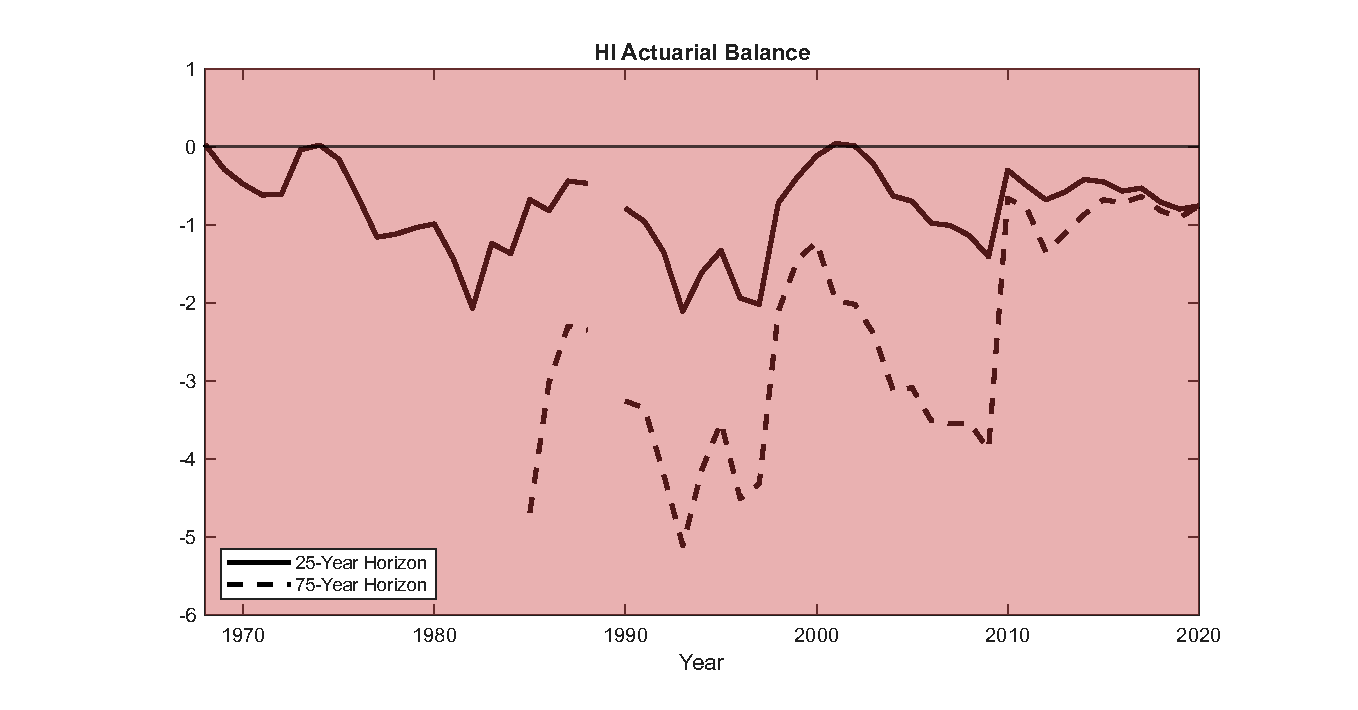
\includegraphics[trim=20mm 00mm 20mm 00mm, clip, scale=0.40]{figures and tables/state_HI_actuarial_25y_75y.pdf}
    \caption{\textbf{Actuarial fiscal position of Medicare Part A (HI).}
    \\[0.5ex]
    \small
    Evolution of the Hospital insurance (HI) actuarial balance over 25-year and 75-year horizons, based on data from the Trustees Reports. The balance is persistently negative, indicating that Medicare Part A is consistently perceived as actuarially unfunded. The 75-year horizon becomes available starting in 1985, while the 1989 observation is omitted because the corresponding Trustees Report did not provide long-horizon projections.
    }
    \label{fig:HI_actuarial}
\end{figure}
Figure \ref{fig:HI_actuarial} shows that the HI actuarial balance is negative throughout our sample, at both the 25- and 75-year horizons.
\paragraph{Fiscal space for discretionary spending.} Discretionary spending has no dedicated account: its backing depends on the resources left after mandatory programs have been financed. We measure these resources with the fiscal democracy index of \cite{Stuerle2010}, henceforth Fiscal index:
$$
\text{Fiscal index} \equiv 1 - \frac{\text{Mandatory spending}+\text{Interest}}{\text{Total revenues}} .     
$$

\begin{figure}[t!]
\begin{subfigure}{0.495\textwidth}
\centering
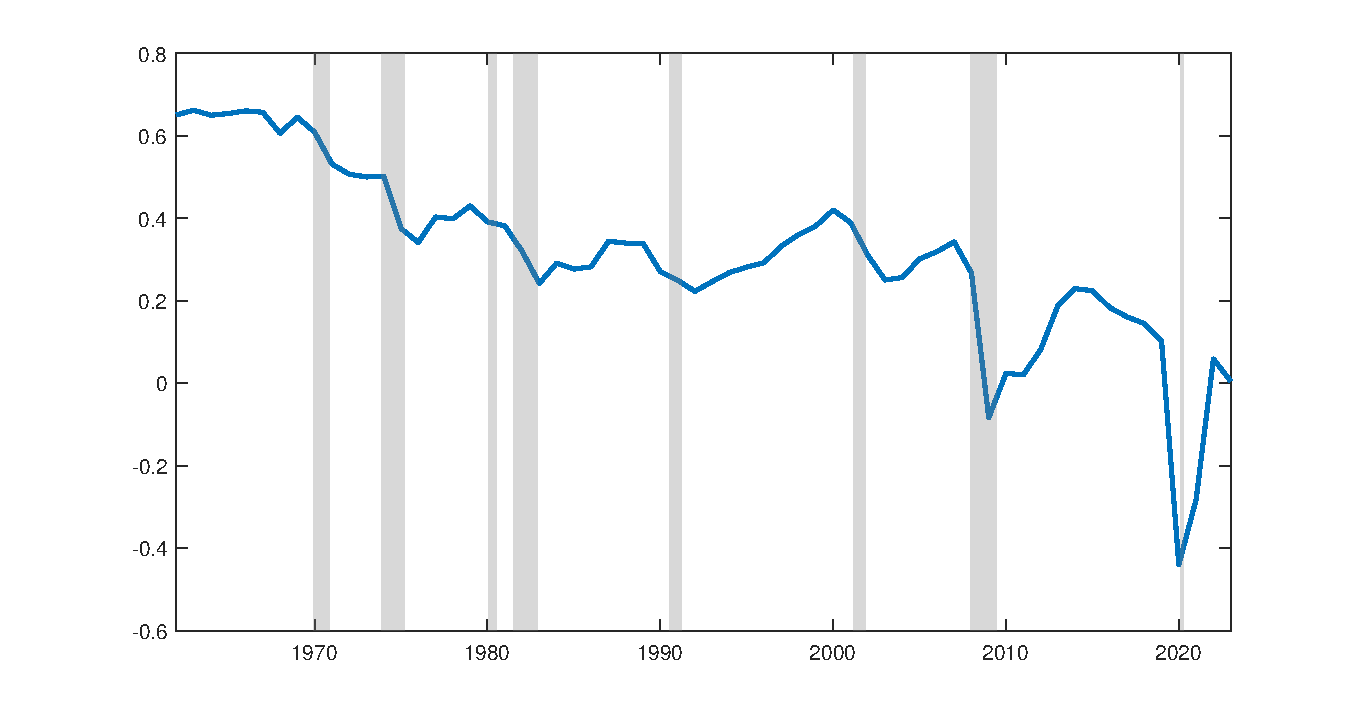
\includegraphics[trim=20mm 00mm 20mm 00mm, clip, scale=0.40]{figures and tables/fiscal_democracy_index.pdf} 
\caption{Fiscal index }
\label{fig:democindex}
\end{subfigure}
\begin{subfigure}{0.495\textwidth}
\centering
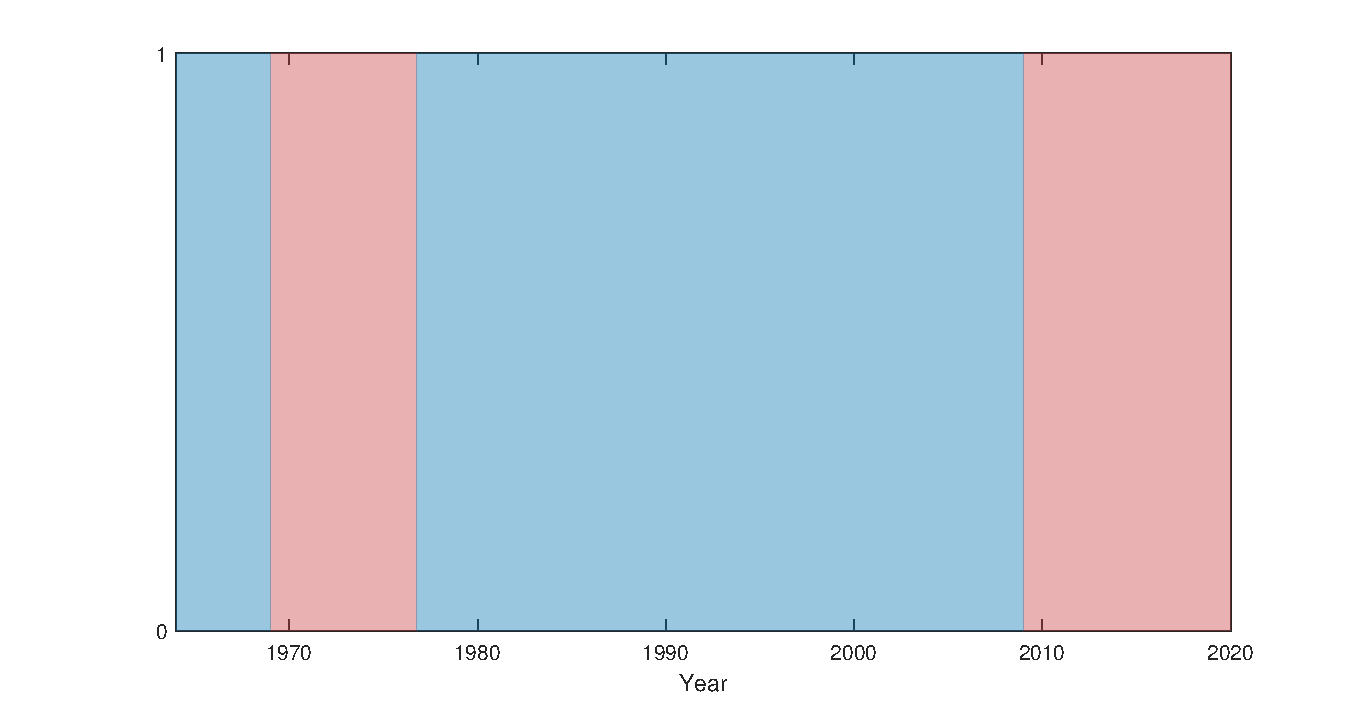
\includegraphics[trim=20mm 00mm 20mm 00mm, clip,scale=0.40]{figures and tables/state_FISCALINDEX.pdf}
\caption{Fiscal capacity for National Defense}
\label{fig:state FI}
\end{subfigure}
\caption{\textbf{Fiscal index and fiscal capacity for National Defense spending.}
\\[0.5ex]
\small
Panel (a): evolution of Fiscal index. Note that the higher the index, the larger are funds available for discretionary spending and hence for ND spending. Grey bands indicate recessions. 
Panel (b): fiscal capacity for National Defense implied by the Fiscal index. Periods of fiscal strain are characterized by decreasing Fiscal index (in red), while periods of no fiscal strain are characterized by non-decreasing Fiscal index (in blue).}
\label{fig:FDI_ND}
\end{figure}
\noindent The higher the index, the stronger the fiscal democracy, as more funds are available for non-predetermined spending. As Figure~\ref{fig:democindex} shows,
the index dropped from 65\% in 1962 to below zero in 2009, with two marked
declines: the first between 1969 and 1976, although the index remained positive,
and the second from 2009 onward, when it turned negative.
% \footnote{``(\ldots) in
% the year after the beginning of the current `financial crisis,' mandatory
% expenses including interest payments exceeded total government income. This was
% caused by a simultaneous decline in revenue and a rapid increase in mandatory
% spending. As a result, all discretionary spending, including military
% expenditure, had to be debt-financed. (\ldots) The global financial crisis that
% began in 2008 has undone any gains in fiscal democracy made in the late 1990s and
% the mid-2000s. In effect, the crisis seems about to eliminate almost completely
% any space for fiscal discretion in the foreseeable future unless governments are
% willing, and able economically and legally, to take up new, additional debt.''
% \citep{StreeckMertens2010}.}
We define periods of scarce fiscal space for discretionary spending as those in
which the Fiscal index declines markedly, namely 1969Q1--1976Q4 and 2009Q1
onward. Red (blue) areas in Figure~\ref{fig:state FI} identify periods of
decreasing (non-decreasing) Fiscal index. Results are robust to assigning fiscal
strain to the post-2009 period only, when the index reached historically low
levels. This period is also characterized by more frequent changes in, and
suspensions of, the debt ceiling (Table~\ref{table:debt_ceiling} in Appendix~\ref{app:sec:suppl}) and, according to
\cite{BFM2023}, by a resurgence of unfunded transfer spending.\footnote{The debt
ceiling limits total federal borrowing. Once reached, Congress must raise or
suspend it to allow the Treasury to meet existing legal obligations.}

\section{The Paradox of Solvency}\label{sec:model}

This section develops a New Keynesian model augmented by  a spending program financed through a dedicated trust fund subject to the asymmetric adjustment rule described in Section~\ref{sec:financing}. The model highlights the implication of the asymmetric nature of the adjustment rule, creating what we name  a `Paradox of Solvency'.
When current-law revenues are expected to cover benefits, the system is considered solvent, so that additional spending need not induce expectations of corrective policy triggering wealth effects. On the contrary, when reserve depletion is anticipated, the same spending news can instead bring forward increases in contributions or reductions in benefits, neutralizing the wealth effect.


The model shows that the fiscal backing of the program---and hence the inflationary effects of news about its spending---depends on its projected actuarial position. The result is general: it applies to any program whose financing follows such a rule. 

The exercise below formalizes the intuition about the effects of this asymmetry and
%. We embed the trust fund in a plain New Keynesian model and 
then map its predictions to the U.S. spending categories studied in the empirical analysis.

\paragraph{Fiscal accounts and asymmetric adjustment.}
Treasury debt consists of publicly held securities, $B^{ON}_k$, and securities held by the trust fund, $B^{OFF}_k$. Both are one-period nominal claims earning the same return. Writing $b^j_k = B^j_k/P_k$ for $j\in\{ON,OFF\}$ and $R_k = i_{k-1}P_{k-1}/P_k$, where $i_k$ is the gross nominal return from $k$ to $k+1$, their real budgets imply
\begin{equation}\label{eq:budgets}
b^{OFF}_k = R_k b^{OFF}_{k-1} + \tau_k + a_k = R_k b^{OFF}_{k-1} + s^{OFF}_k,
\qquad
b^{ON}_k = R_k b^{ON}_{k-1} - \bar s^{ON} - s^{OFF}_k .
\end{equation}
The trust-fund balance $s^{OFF}_k=\tau_k+a_k$ consists of the current-law balance
$\tau_k$ (contributions minus benefits) and a correction $a_k\geq 0$, which
represents additional contributions or equivalent benefit reductions. The primary
surplus outside the program, $\bar s^{ON}$, is held fixed within each experiment.
Trust-fund securities cancel upon consolidation: their accumulation changes the
Treasury's financing needs but does not create an additional private claim on the
government.\footnote{In practice, the trust funds hold special-issue Treasury
securities, and the cash exchanged for them enters the General Fund. The common one-period return abstracts from their actual maturity structure; see the SSA's \href{https://www.ssa.gov/oact/progdata/fundFAQ.html}{Trust Fund FAQs} and \href{https://www.ssa.gov/OACT/ProgData/specialissues.html}{description of special issues}.}

At date 0, the government releases current-law projections of the program's balance for $k=1,\dots,K$, where $K\geq 1$ is the projection horizon; beyond $K$, the balance is projected to remain at its date-$K$ value. These projections exclude future corrective policy.\footnote{The distinction mirrors the use of current-law financing projections to assess scheduled benefits. See the Social Security Administration's discussion of \href{https://www.ssa.gov/policy/docs/ssb/v70n3/v70n3p111.html}{program solvency}.} News is a revision of these projections, such as an announced benefit expansion or an upward revision in the projected number of beneficiaries.

Let $\underline{b}>0$ be a reserve floor. The authority intervenes at the first projected breach $K^*$ of the floor, evaluated under current law. Before $K^*$, reserves follow their current-law path. From $K^*$ onward, the correction raises reserves to a target $m_k$ such that (i) reserves never fall below the floor over the projection horizon, $m_k\geq\underline{b}$ for $K^*\leq k\leq K$, and (ii) reserves equal the floor beyond the horizon, $m_k=\underline{b}$ for $k>K$. 
The correction schedule is therefore defined beyond the finite actuarial horizon as well, given the expected flat continuation after $K$. Setting $m_{K}=\underline b$ gives the smallest terminal reserve target consistent with stabilization. 
Backward recursion from $m_{K}$ yields the adjustment required at $K^*$ to ensure that reserves remain at or above $\underline b$ for the remainder of the projection horizon and equal $\underline b$ after K. 
%Targets are obtained by backward recursion from $m_K=\underline{b}$ (Appendix~\ref{sec:app:model}). 
If no breach is projected, $K^*=\infty$ and no correction occurs. The correction is
\begin{equation}\label{eq:rule}
a_k =
\begin{cases}
0, & 0\leq k<K^*,\\[2pt]
\left[m_k - b^{pre}_k\right]^+, & k\geq K^*,
\end{cases}
\qquad [z]^+\equiv\max\{z,0\},
\end{equation}
where $b^{pre}_k$ denotes reserves before correction. This rule formalizes the asymmetry: it implies a credible anticipated adjustment when reserve depletion is projected (Figure~\ref{fig:correction_rule_a}), but no offsetting reduction in contributions when reserves are ample (Figure~\ref{fig:correction_rule_b}). Its front-loaded structure is consistent with the actuarial notion of solvency used by the Social Security Trustees, who assess trust-fund ratios against a threshold over the projection period and require them to be stable at its end (Board of Trustees, 2026); our floor $\underline{b}$ and horizon $K$ play the same roles.\footnote{Both results are robust to the timing of the correction. Under projected depletion, any rule that returns reserves to the floor irrespective of the news, including one that corrects period by period from the first projected breach onward, leaves the present value of the program's balances unchanged and therefore delivers neutrality. Under ample reserves, no breach is projected and no correction occurs under either rule, so the inflationary response is identical. We have verified numerically that the two rules yield the same equilibrium responses in both scenarios.}
\begin{figure}[H]

\centering
\pgfplotsset{
  resplot/.style={
    width=\linewidth, axis lines=left, axis line style={-{Stealth[length=5pt]}, gray},
    ytick=\empty, xmin=0, xmax=58, xlabel={$k$},
    xlabel style={at={(axis description cs:1,0)}, anchor=north east},
    tick style={draw=none}, clip=false, samples=120,
    tick label style={font=\footnotesize}, label style={font=\footnotesize},
    legend style={at={(0.5,-0.2)}, anchor=north, draw=none, legend columns=-1,
      /tikz/every even column/.append style={column sep=12pt}, font=\footnotesize},
  },
  /pgf/declare function={
    bpa(\x) = (\x<=40)*(3-0.04*\x-0.0015*\x^2) + (\x>40)*(-1-0.16*(\x-40));
    ma(\x)  = (\x<=40)*(5-0.04*\x-0.0015*\x^2) + (\x>40)*1;
    bpb(\x) = (\x<=40)*(2+(1-\x/40)^2) + (\x>40)*2;
  },
}

\begin{subfigure}{\linewidth}
\centering
\resizebox{0.75\linewidth}{!}{%
\begin{tikzpicture}
\begin{axis}[resplot, height=6cm, ymin=-3.6, ymax=3.4,
  xtick={0,25.54,40}, xticklabels={$0$,$K^*$,$K$}]
  \addplot[name path=M, draw=none, forget plot, domain=25.54:55] {ma(x)};
  \addplot[name path=P, draw=none, forget plot, domain=25.54:55] {bpa(x)};
  \addplot[resteal, fill opacity=0.15, forget plot] fill between[of=M and P];
  \draw[gray!60, densely dotted] (axis cs:25.54,-3.6) -- (axis cs:25.54,3.4);
  \draw[gray!60, densely dotted] (axis cs:40,-3.6) -- (axis cs:40,3.4);
  \draw[floororange, dashed, thick] (axis cs:0,1) -- (axis cs:57,1);
  \addplot[resteal, very thick, domain=0:25.54] {bpa(x)};
  \addlegendentry{reserves with correction}
  \addplot[pregray, thick, dashed, domain=25.54:55] {bpa(x)};
  \addlegendentry{current law, no correction}
  \addlegendimage{area legend, fill=resteal!15, draw=resteal!15}
  \addlegendentry{cumulated corrections}
  \addplot[resteal, very thick, domain=25.54:55, forget plot] {ma(x)};
  \draw[resteal, very thick] (axis cs:25.54,1) -- (axis cs:25.54,3);
  \fill[floororange] (axis cs:25.54,1) circle (2.2pt);
  \fill[resteal] (axis cs:40,1) circle (2.2pt);
  \node[font=\footnotesize, align=center] at (axis cs:12.5,4.1) {Current law\\ $a_k=0$};
  \node[font=\footnotesize, align=center] at (axis cs:33,4.1) {Correction\\ $m_k\ge\underline{b}$};
  \node[font=\footnotesize, align=center] at (axis cs:49,4.1) {Beyond the horizon\\ $m_k=\underline{b}$};
  \node[font=\footnotesize, anchor=east] at (axis cs:25,2) {$a_{K^*}$};
  \node[font=\footnotesize, anchor=south west] at (axis cs:0.5,1) {floor $\underline{b}$};
  \node[font=\footnotesize, anchor=north east] at (axis cs:25,0.85) {first projected breach};
  \node[font=\footnotesize, align=left, anchor=west] at (axis cs:41,2.1) {backward recursion\\ from $m_K=\underline{b}$};
  \node[font=\footnotesize, align=center] at (axis cs:33,-0.9) {$a_k=0$\\ for $K^*<k\le K$};
  \node[font=\footnotesize, align=center] at (axis cs:50,-0.6) {$a_k>0$:\\ covers each\\ period's deficit};
\end{axis}
\end{tikzpicture}%
}
\caption{Projected breach at $K^*$}
\label{fig:correction_rule_a}
\end{subfigure}

\vspace{0.6em}

\begin{subfigure}{\linewidth}
\centering
\resizebox{0.75\linewidth}{!}{%
\begin{tikzpicture}
\begin{axis}[resplot, height=4.3cm, ymin=0, ymax=3.6,
  xtick={0,40}, xticklabels={$0$,$K$}]
  \addplot[name path=B, draw=none, forget plot, domain=0:57] {bpb(x)};
  \addplot[name path=F, draw=none, forget plot, domain=0:57] {1};
  \addplot[pattern=north east lines, pattern color=excessamber!60, draw=none, forget plot]
    fill between[of=B and F];
  \draw[gray!60, densely dotted] (axis cs:40,0) -- (axis cs:40,3.6);
  \draw[floororange, dashed, thick] (axis cs:0,1) -- (axis cs:57,1);
  \addplot[resteal, very thick, domain=0:57] {bpb(x)};
  \addlegendentry{reserves under current law (no correction)}
  \addlegendimage{area legend, pattern=north east lines, pattern color=excessamber!60, draw=excessamber!60}
  \addlegendentry{reserves above the floor, not returned}
  \node[font=\footnotesize, fill=white, inner sep=2pt] at (axis cs:26,1.5) {excess above $\underline{b}$: no offsetting reduction in contributions};
  \node[font=\footnotesize, anchor=north west] at (axis cs:0.5,1) {floor $\underline{b}$};
  \node[font=\footnotesize, align=center] at (axis cs:50,3.1) {$K^*=\infty,\ a_k=0$\\ no projected breach};
\end{axis}
\end{tikzpicture}%
}
\caption{No projected breach, $K^*=\infty$}
\label{fig:correction_rule_b}
\end{subfigure}

\caption[Anticipated correction rule for Social Security reserves]{\textbf{Anticipated correction rule for Social Security reserves.}\\
\small Panel~(a): reserves follow current law until the first projected breach $K^*$, when the correction $a_{K^*}$ lifts them above the floor so that they decline to $\underline{b}$ exactly at $K$; beyond $K$, $a_k$ covers the recurring deficits, keeping reserves at $\underline{b}$. The shaded area shows cumulated corrections relative to the current-law path. Panel~(b): reserves never fall below $\underline{b}$, so $K^*=\infty$ and $a_k=0$.}
\label{fig:correction_rule}
\end{figure}


\paragraph{Private sector and monetary policy.}
A representative household pools resources across young members, who supply labor and pay contributions, and old members, who receive benefits. The household takes the correction rule (\ref{eq:rule}) as given: it anticipates $a_k$ whenever a breach is projected and no correction otherwise. With Calvo price setting, the equilibrium conditions at any date $k$ after a date-0 announcement are described by the standard three-equation New Keynesian model:\footnote{For simplicity, taxes and benefits (as well as their corrections) are lump-sum. A demographic productivity offset keeps natural output constant, so revisions to the projected beneficiary share affect demand through the program's finances alone. Appendix~\ref{sec:app:model} describes the details of the model, as well as the fiscal rule and the solution method.}
\begin{equation}\label{eq:nk}
y_k = y_{k+1} - \sigma^{-1}\left(\hat\imath_k - \pi_{k+1}\right),
\qquad
\pi_k = \beta\pi_{k+1} + \kappa y_k,
\qquad
\hat\imath_k = \phi\,\pi_k,
\quad 0\leq\phi<1,
\end{equation}
where $y_k$ is the log output gap, $\pi_k$ is log inflation, and $\hat\imath_k$
is the deviation of the log gross nominal interest rate from $\log r$, with
$r=\beta^{-1}$ (assuming zero steady-state inflation). Monetary policy is
passive.\footnote{Given that the non-program surplus $\bar s^{ON}$ is held fixed, fiscal policy is active and determinacy requires passive monetary policy ($\phi<1$). This configuration is consistent with the evidence for the pre-Volcker period \citep[e.g.,][]{CGG00, DavigLeeper2007,Bianchi2012}, which covers the solvency regime of Social Security. The neutrality result under projected depletion does not hinge on this assumption: since the correction rule leaves the present value of the program's balances unchanged, the news is fiscally funded and would be neutral under an active-monetary/passive-fiscal configuration as well.}
Once the announcement arrives, there is no further uncertainty.\footnote{The parameter $\sigma$ is the inverse intertemporal elasticity of substitution, $\beta$ is the household discount factor, $\kappa$ is the slope of the New Keynesian Phillips curve, and $\phi$ measures the nominal interest rate response to inflation. $\kappa=(1-\theta)(1-\beta\theta)(\sigma+\nu)/\theta$, where $\theta$ is the Calvo probability that a firm cannot reset its price and $\nu$ is the inverse Frisch elasticity of labor supply. In the calibration below, a period is one year and we set $\beta=0.96$, $\sigma=\nu=1$, $\theta=0.6$ and $\phi=0.5$.}

\paragraph{The paradox of solvency.}
Publicly held debt, $B^{ON}_k$, is the government liability relevant for price-level determination. Household transversality implies:
\begin{equation}\label{eq:valuation}
\frac{i_{-1}B^{ON}_{-1}}{P_0}
= \sum_{k=0}^{\infty} q_k
\underbrace{\left(\bar s^{ON} + \tau_k + a_k\right)}_{\text{consolidated primary surplus}}
= PV(\bar s^{ON}) + PV(\tau) + PV(a),
\end{equation}
where $PV(x)\equiv\sum_{k=0}^\infty q_k x_k$ and $q_k$ is the household discount
factor.  In each scenario, the outside surplus $\bar s^{ON}$ is set so that (\ref{eq:valuation}) holds with zero inflation along the no-news path. 
Expected trust-fund surpluses are therefore already reflected in the initial price level: a known path of surpluses, however large, generates neither inflation nor deflation over time. Only revisions to that path move prices, and all responses below are measured relative to each scenario's own no-news path.

Consider news that lowers future current-law balances, $\Delta PV(\tau)<0$. When
reserves are ample, no breach is projected and $a_k=0$: the news lowers the
present value of consolidated surpluses one-for-one. Since $\bar s^{ON}$ does not
respond, (\ref{eq:valuation}) requires a higher price level, and the news
generates wealth effects and inflation. When depletion is projected, instead, the
correction rule implies $\Delta PV(\tau+a)=0$: the deterioration is offset by
anticipated corrections, the present value of surpluses is unchanged, and the
news is neutral. The same news is thus fiscally unfunded when the program is
actuarially funded, and fiscally funded when it is actuarially unfunded. This is
the \emph{paradox of solvency}.

\paragraph{A numerical illustration.}
We illustrate the mechanism by simulating the model under ample reserves and
under projected reserve depletion. The exercise is not a quantitative account of
any specific episode. Both scenarios start with public debt of 60\% and reserves
of 10.6\% of reference GDP; the reserve floor $\underline{b}$ is 8\%. The
ample-reserve reference has a current-law surplus of 0.6\% of GDP, whereas the
projected-depletion reference has a deficit of 0.7\%. In each case, the news
leaves the date-0 balance unchanged and lowers future balances by 0.015\% of
reference GDP per year through the projection horizon $K=10$; the terminal
reduction of 0.15\% persists thereafter. The news can be read as an announced
benefit expansion; in Appendix~\ref{sec:app:model} it is implemented as an upward
revision in the projected share of beneficiaries, which has the same effect on
$\tau_k$. Figure~\ref{fig:paradox} displays the implied dynamics.

With ample reserves, the revised balance remains positive and no breach is
projected, so $K^*=\infty$ and $a_k=0$, as in Figure~\ref{fig:correction_rule_b}. The news
lowers the present value of fiscal surpluses, and the price level must rise to
restore the consolidated government's intertemporal budget constraint. Higher
benefits raise perceived private wealth and consumption, pushing up prices and,
given nominal rigidities, output. Inflation rises by 3.15 percentage points and
output by 1.9\% on impact; the response decays over time, while reserves keep
growing, although more slowly than without news.

With projected depletion, the same news moves the first projected breach $K^*$
from year 8 to year 7. The correction raises reserves to 9.4\% of reference GDP,
after which they decline to the floor, as in Figure~\ref{fig:correction_rule_a}. Because the
correction absorbs the lower current-law balances in present value---first
through the initial adjustment $a_{K^*}$ and then period by period beyond
$K$---it exactly offsets the deterioration. Inflation and output remain at their
no-news values.

\begin{figure}[tbp]
 \centering
 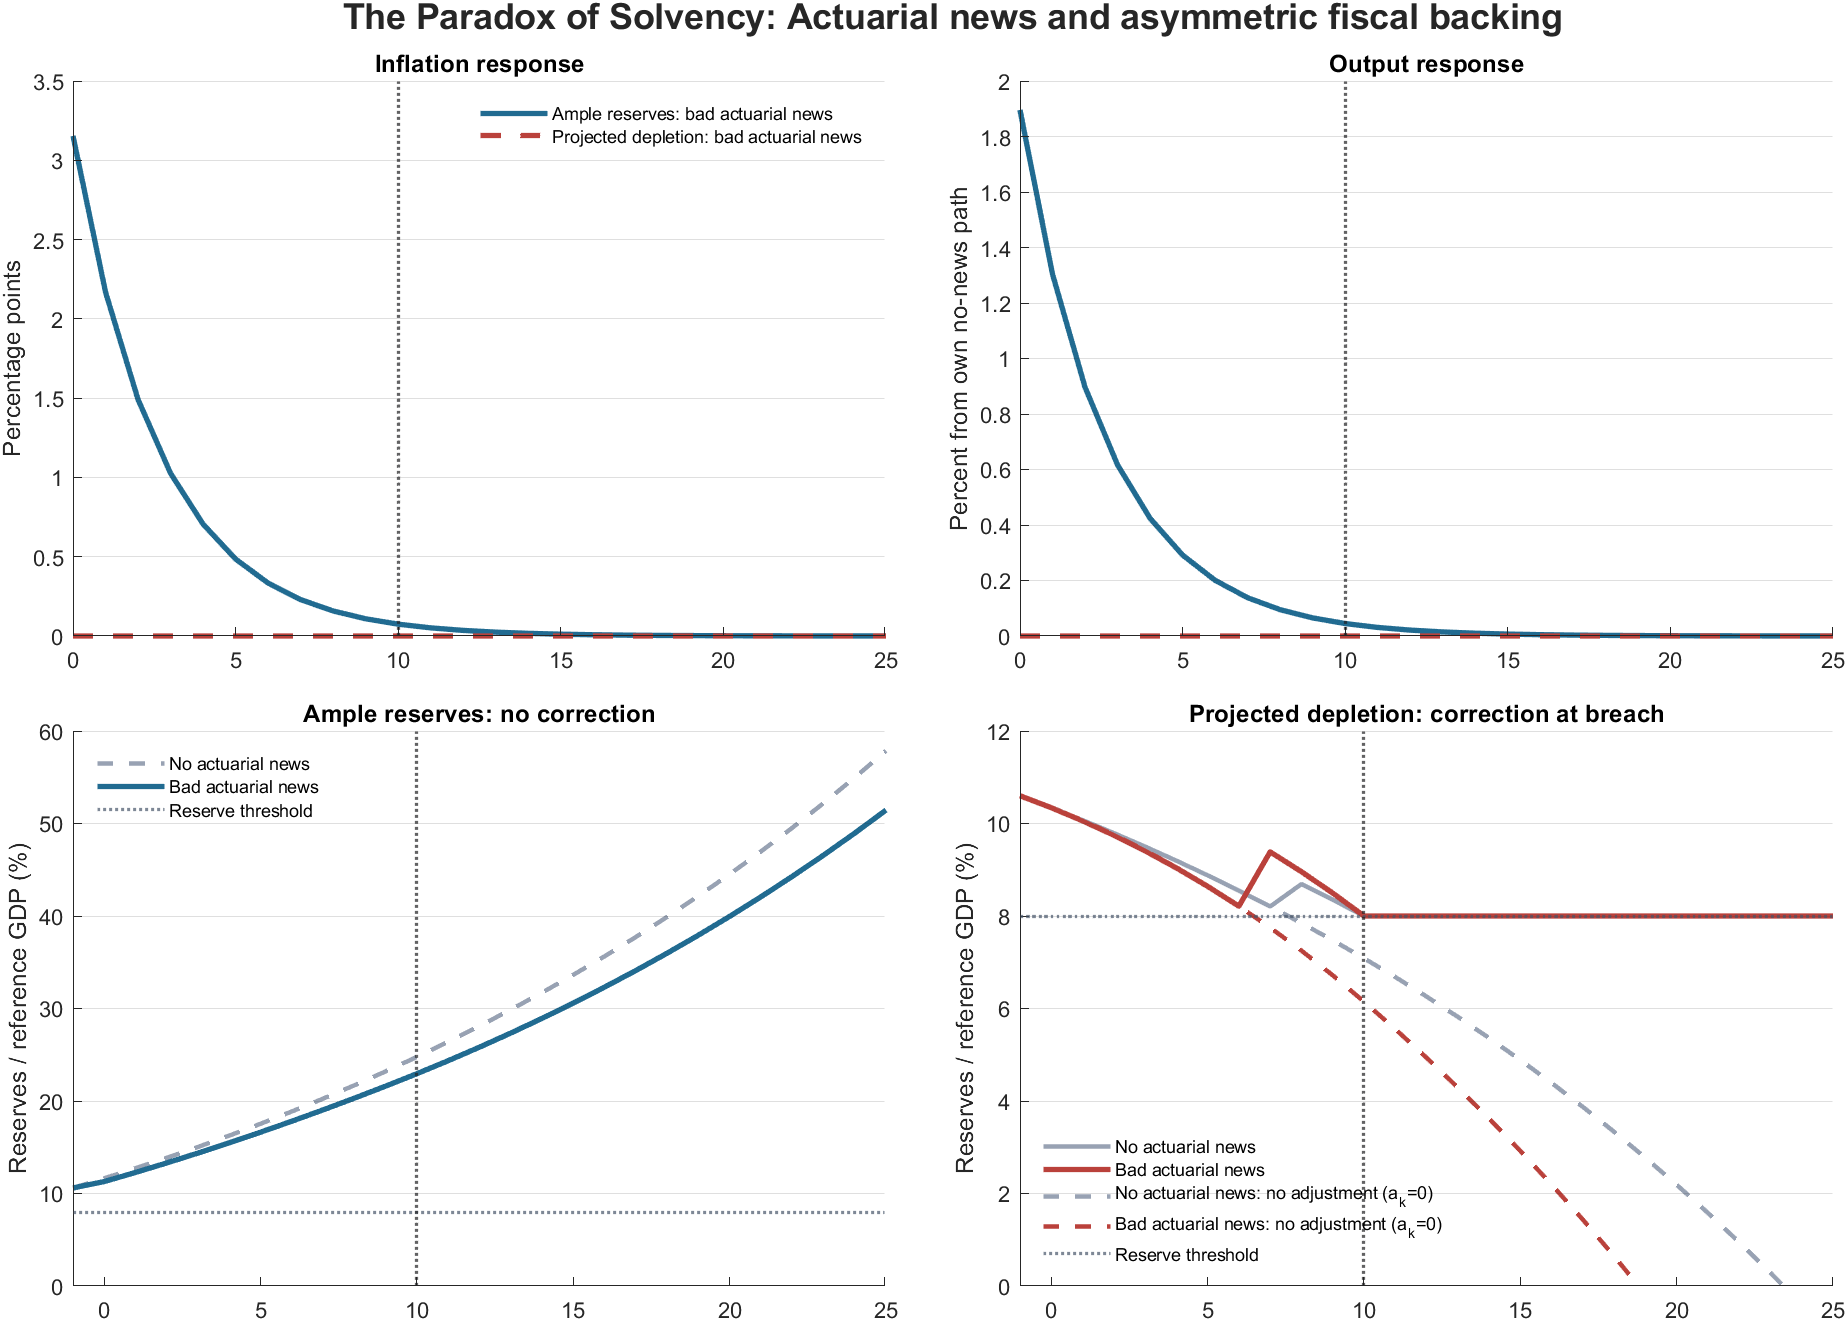
\includegraphics[width=\linewidth]{figures and tables/sim_model_GA.png}
 \caption{\textbf{The Paradox of Solvency: Actuarial news and asymmetric fiscal backing.}
 \small The same permanent deterioration in current-law balances under ample reserves (blue) and projected depletion (red).  Inflation and output are deviations from each scenario's no-news equilibrium. Reserve stocks are percentages of reference GDP. Gray paths denote no news; in the depletion panel solid paths include anticipated corrections and dashed paths suppress them. Dashed counterfactuals stop at zero reserves. Dotted lines indicate the reserve floor and the actuarial horizon $K=10$ (cf.\ Figure~\ref{fig:correction_rule}).}
\label{fig:paradox}
 \label{fig:Scenario_socsec}
\end{figure}

\paragraph{Mapping to U.S. spending programs.}
The model maps directly onto the financing rules described in
Section~\ref{sec:background}. Social Security before 1974, when the OASDI
actuarial balance was positive, corresponds to the ample-reserve case; after
1974, when depletion became anticipated, it corresponds to the projected-depletion
case. Medicare Hospital Insurance, whose actuarial balance has been negative
throughout our sample, has always been in the projected-depletion case.
Medicare Parts B and D and Medicaid represent a limiting case in which the
correction is automatic and occurs every period through general revenues.

National defense lies outside the model, as it has no dedicated account. Its
backing depends on whether the general revenues left after mandatory programs
are financed can absorb additional spending. The underlying principle is the
same---a spending shock is fiscally funded only if a credible mechanism
anticipates future adjustment---but for discretionary spending it is the scarcity
of fiscal space, rather than abundance, that removes such a mechanism.

The model therefore delivers sharp predictions for the empirical analysis. News about Social Security spending should generate inflationary and expansionary responses before 1974, when the system was actuarially funded, and Ricardian responses thereafter. News about Medicare and Medicaid spending should generate Ricardian responses throughout the sample. News about defense spending should generate inflationary and expansionary responses only when fiscal space for discretionary spending is scarce.


Two qualifications apply. First, neutrality under projected depletion is conditional on credible and sufficient correction: if such correction is no longer expected, inflationary wealth effects can reappear. Second, holding Treasury securities does not by itself establish fiscal backing. The OASI and DI funds are legally distinct and need not share the same outlook; their aggregation here isolates the mechanism, not their separate depletion dates.\footnote{The \href{https://www.ssa.gov/oact/tr/2026/II_E_conclu.html}{2026 Trustees Report, Section II.E} projects OASI depletion in 2032 but no DI depletion within its 75-year horizon. Its combined depletion date of 2034 assumes legislation permitting transfers between the funds. These projections concern current-law financing, not the fiscal response households expect.}

%In this Section, we use a plain New Keynesian model augmented by a reserve fund to highlight the mechanism that can account for the contrasting responses before and after 1974. 
%Social Security's financing arrangements distinguish actuarial solvency from fiscal backing. 
%The key distinction is the following asymmetry. When current-law revenues are expected to cover benefits, additional spending need not induce expectations of corrective policy. When reserve depletion is anticipated, the same spending news can instead bring forward increases in contributions or reductions in benefits. 
%This asymmetry in fiscal backing creates a `Paradox of Solvency'. An increase in benefits triggers wealth effects, when the system is considered solvent, that is, when revenues are expected to be sufficient so that no future increase in contributions is expected.
%Hence, a wealth effect arises when the system is considered solvent.
%On the contrary, when the system is projected to be insolvent, an expansion in benefits widens the shortfall, so that an increase in future contributions or taxes is expected to cover the loss, neutralizing the wealth effect.
%The simple exercise below formalizes the intuition about the effects of this asymmetry. 
%and it is not a quantitative account of either episode.



%\paragraph{Fiscal accounts and asymmetric adjustment.}
%Treasury debt consists of publicly held securities, $B_k^{ON}$, and securities held by the trust fund, $B_k^{OFF}$. Both are one-period nominal claims earning the same return. Writing $b_k^j=B_k^j/P_k$ for $j\in\{ON,OFF\}$ and $R_k=i_{k-1}P_{k-1}/P_k$, where $i_k$ is the gross nominal return from $k$ to $k+1$, their real budgets imply:
%\begin{align}
% b_k^{OFF}&=R_k b_{k-1}^{OFF}+\tau_k+a_k=R_k b_{k-1}^{OFF}+s^{OFF}_k, &%\label{eq:ga_reserves}\\
 %\quad b_k^{ON}&=R_k b_{k-1}^{ON}-\bar s^{ON}-s^{OFF}_k. \label{eq:ga_public_debt}
%\end{align}
%The Social Security balance is $s^{OFF}_k=\tau_k+a_k$ where $\tau_k$ is the current-law balance (contributions minus benefits) and $a_k\geq0$ denotes additional contributions, or equivalent benefit reductions. We assume that the non-Social-Security primary surplus $\bar s^{ON}$ is fixed within each experiment. Trust-fund securities cancel upon consolidation: their accumulation changes the Treasury's financing needs but does not create an additional private claim on the government.\footnote{In practice, Social Security holds special-issue Treasury securities, and the cash exchanged for them enters the General Fund. The common one-period return abstracts from their actual maturity structure; see the SSA's \href{https://www.ssa.gov/oact/progdata/fundFAQ.html}{Trust Fund FAQs} and \href{https://www.ssa.gov/OACT/ProgData/specialissues.html}{description of special issues}.}

%At date $0$, the government releases the path of the projected fraction of old members at future dates $k = 1, \dots, K$, where $K\geq1$ is the projection horizon. Revisions of this path constitute anticipated demographic news. Beyond the projection horizon, projections assumes the old-age share to remain flat at its at its date-$K$ value. These are current-law projections that exclude future corrective policy.\footnote{The distinction mirrors the use of current-law financing projections to assess scheduled benefits. See the Social Security Administration's discussion of \href{https://www.ssa.gov/policy/docs/ssb/v70n3/v70n3p111.html}{program solvency}.}


%To construct the correction schedule, let $\underline b>0$ be a reserve floor. Breaches of the floor
%are evaluated under current law, without future corrections.
%such that when reserve hits this lower bound the fiscal authority intervenes to avoid further reserve depletion. 
%The authority intervenes at the first projected breach $K^*$ of the reserve floor $\underline b.$ 
%Before $K^*$, reserves follow their current-law evolution. From $K^*$ onward, the correction raises reserves to a level $m_{k}$ so that: (i) reserve are never below the floor over the projection horizon, i.e., $m_{k}\geq\underline b\quad\text{for all } K^* \leq k \leq K$ ; (ii) given the expected flat continuation after $K$, reserve are at the floor beyond the projection horizon, i.e.,  $m_{k}=\underline b$ for $k>K$. The correction schedule is therefore defined beyond the finite actuarial horizon as well.

%Setting $m_{K}=\underline b$ gives the smallest terminal reserve target consistent with stabilization. 
%Backward recursion from $m_{K}$ yields the adjustment required at $K^*$ to ensure that reserves remain at or above $\underline b$ for the remainder of the projection horizon and equal $\underline b$ after K. The minimum reserve targets are computed using the same anticipated gross real return as the reserve projection. If no breach is projected, $K^*=\infty$ and no correction occurs. The correction is therefore
%\begin{equation}
 %a_k=\begin{cases}
 %0,&0\leq k<K^*,\\
 %[m_k-b_k^{pre}]_+,&k\geq K^*,
 %\end{cases}
 %\qquad [z]_+\equiv\max\{z,0\},
 %\label{eq:ga_adjustment}
%\end{equation}
%where $b_k^{pre}$ denotes reserves before correction. An intervention can therefore raise reserves above the floor before they decline toward it (Figure~\ref{fig:correction_rule}, panel~a). This rule formalizes the key asymmetry. Under our assumptions, it implies a credible anticipated adjustment within Social Security when reserve depletion is anticipated, while it imposes no offsetting tax reduction when reserves are ample (panel~b).

%The front-loaded adjustment is consistent with the actuarial notion of solvency used by the Social Security Trustees, who assess trust fund ratios against a threshold over the entire projection period and require them to be stable at its end \citep{trustees2026}. Our floor $\underline{b}$ and horizon $K$ play the same roles.\footnote{Both results are robust to the timing of the correction. Under projected depletion, any rule that returns reserves to the floor irrespective of the news, including one that corrects period by period from the first projected breach onward, leaves the present value of Social Security balances unchanged and therefore delivers neutrality. Under ample reserves, no breach is projected and no correction occurs under either rule, so the inflationary response is identical. We have verified numerically that the two rules yield the same equilibrium responses in both scenarios.} 

%\usepackage{float}   % preambolo
%\begin{figure}[H]

\section{Empirical Analysis\label{sec: method}} 
\paragraph{Shock construction.} We use data from the U.S. federal budget to construct a measure of government spending shocks. The fiscal year runs from October 1 to September 30 of the following year and it is named after the calendar year in which it ends.\footnote{For example, fiscal year 2025 begins on October 1, 2024, and ends on September 30, 2025.} The U.S. Federal Budget for a given fiscal year is typically released in March/April of the previous year. Because the budget is released before the start of the fiscal year, many of the data points and financial projections it contains are estimates. We exploit these estimates to construct our anticipated measure of government spending shock. 

Following \cite{ForniGambetti2016}, we construct a quarterly measure of the one-year-ahead expected growth rate in real spending by subcategory. For instance, for Defense spending in 2022Q1, the measure is defined as:
     $$f^\text{ND}_{2022q1} = \log\left\{\frac{\mathbb{E}_{2022q1}(\text{real defense spending in 2023})}{\mathbb{E}_{2022q1}(\text{real defense spending in 2022})}\right\}$$
This measure is non-zero only in the quarter in which the budget is released; it is set to zero in all other quarters. We construct such a measure for the two broad spending categories (mandatory and discretionary), as well as for key subcategories such as Medicare and Medicaid combined, National Defense, and Social Security.

An important caveat must be addressed here: projected government spending may adjust to expected macroeconomic conditions, which would render our measure of fiscal shocks endogenous. To mitigate this concern, we adopt two alternative strategies. First, still taking National Defense as an example, we regress $f^{\text{ND}}_t$ on the projected growth rate of real GDP reported in the budgets, and denote the residuals of this regression as $f^{\text{ND, purged}}_t$. Second, we exploit information from the Survey of Professional Forecasters (SPF), regressing $f^{\text{ND, purged}}_t$ on the expected growth rate of GDP and the expected change in unemployment, and denote the corresponding residuals as $f^{\text{ND, SPF-purged}}_t$. The same procedure is applied to the fiscal shocks for each subcategory of spending. The time series of both the original and the purged fiscal shocks for all spending subcategories are reported in Appendix \ref{sec:purged}. The series are highly similar, and the correlation between the original and purged shocks is consistently very high (always above 0.95), supporting the view that unpurged shocks still capture the exogenous component of government spending and suggesting that the potential endogeneity problem is not particularly severe. In the main text, we therefore report only the impulse responses to the baseline unpurged shocks, while leaving those obtained from the purged shocks to Appendix \ref{sec:purged}.%
\footnote{A second issue arises from the fact that budgets report spending projections only in nominal terms, requiring a deflator to convert them into real quantities. However, projections of the GDP deflator are available only from 1976 onwards. Consequently, we construct our baseline measure of fiscal shocks using the actual GDP deflator series. As a robustness check, we also generate an alternative fiscal shock series using an expected GDP deflator series that we build by combining soft information from the budgets (1963–1968), SPF forecasts (1969–1975), and the projected deflator reported in the budgets (1976 onwards). %Appendix XXX displays the one-year actual and expected inflation series, as well as impulse response functions to the fiscal shock incorporating the expected deflator. 
Results are highly consistent across specifications. Therefore, the main text only reports the impulse responses to our baseline measures of fiscal shocks, which rely on actual inflation. Results based on projected inflation are available from the authors upon request.}

\paragraph{Local projections.} We employ the measures of fiscal shocks within  \citetpos{Jorda} local projection framework to evaluate the macroeconomic effects of anticipated government spending, disaggregated by subcategory.  More in detail, each subcategory-specific measure is used as the shock variable in a series of local projections regressions, allowing us to estimate impulse response functions for a range of macroeconomic outcomes. 

We consider both linear and state-dependent local projections. In the linear case, the local projection for horizon $h$ is specified as  
%We use \cite{Jorda}'s local projections to compute impulse responses to a shock of our measures of anticipated and disaggregated government spending shocks. The linear model looks as follows:
\begin{equation} \label{eq:linearLP}
y_{t+h} = \alpha_h + \beta_h x_t + \sum_{i=1}^p \bm{\gamma}_i' \bm{w}_{t-i} + v_{t+h},
\end{equation}
where $y_t$ is the outcome variable, $x_t$ is the measure of disaggregated government spending shocks, and $\bm{w}_t$ is the set of control variables. The outcomes include quarterly NIPA variables such as aggregate federal government purchases, aggregate federal transfers, GDP, private consumption and private investment. 
Following \citet{Ramey2016}, we adopt the \citetalias{GordonKrenn2010} transformation: all NIPA variables are first deflated by the GDP deflator and then divided by potential GDP, estimated as a quadratic trend fitted on real GDP.
We also consider other variables such as inflation, the differential between the interest rate and output growth ($r-g$), and debt over GDP. The combined reactions of the interest-rate–growth differential ($r-g$), inflation, output, and the debt-to-GDP ratio to anticipated fiscal shocks reveal the type of monetary–fiscal coordination -- indicating whether the regime is one of monetary or fiscal dominance.\footnote{The ‘growth-augmented Taylor principle' \citep[see][]{ElfsbackaMcClung2024} claims that, to maintain economic stability under a debt-stabilizing fiscal policy, central banks must raise ($r-g$). This helps control inflation, as higher growth can contribute to inflationary pressures. In contrast, under a fiscal authority which does not stabilize debt, central banks can stabilize the public debt by letting $r-g$ fall with inflation.}
The set of controls always includes four lags of output, of the outcome variable, and of the shock, to account for the presence of autocorrelation on our measures of anticipated government spending. We also include lagged transfers when computing impulse responses to MM and SS shock, as these subcategories are classified in NIPA tables as government social benefits to persons. We instead include lagged government purchases  when computing impulse responses to ND and discretionary spending shocks. Finally, we include both transfers and purchases in the case of mandatory spending shocks.\footnote{While most mandatory spending consists of transfers to individuals, a small share includes government purchases of services, such as administrative costs for programs like Medicare, which are not classified as transfers. Results are barely unchanged if we use just transfers.}
Results are robust to including taxes as controls.
%varies according to the spending domain we consider. Therefore, it contains 4 lags of outcome, $TR$, and $Y$ when computing IRFs to SS (and MM) shocks, 4 lags of outcome, $G$, and $Y$ when computing IRFs to ND and discretionary shocks, 4 lags of outcome, $TR$, $G$ and $Y$ when computing IRFs to mandatory shocks. 

Following \citet{RameyZuba2018}, we also account for state dependence by incorporating several state variables in our local projection framework. These variables allow us to assess whether the impulse responses to an anticipated shock in a specific spending category vary depending on whether the fiscal capacity in that category is high or low. The state variables are those described in Section \ref{sec:actuarial_soundeness}: the 75-year OASDI actuarial balance for Social Security and the Fiscal index for National Defense. Medicare and Medicaid, whose fiscal backing does not vary over time, are analyzed with linear local projections. For the model with state dependence, we estimate a set of regressions such as
\begin{align}
y_{t+h} 
&= \mathcal{I}_{\{z_{t-1}=1\}}\left(\alpha^1_{h} + \beta^1_{h} x_t + \sum_{i=1}^p \left(\bm{\gamma}^1_{h,i}\right)' \bm{w}_{t-i}\right) \nonumber \\ 
&\quad+ \mathcal{I}_{\{z_{t-1}=0\}}\left(\alpha^0_{h} + \beta^0_{h} x_t + \sum_{i=1}^p \left(\bm{\gamma}^0_{h,i}\right)' \bm{w}_{t-i}\right)
+ v_{t+h},
\label{eq:SDLP}
\end{align}
where $\mathcal{I}$ is a dummy variable that indicates the state of the economy when the shock hits. In particular, coefficient $\beta^1_h$ is the impulse response at horizon $h$ conditional on the subcategory-specific fiscal capacity being low ($z_t=1$), signaling fiscal strain; conversely, coefficient $\beta^0_h$ is the impulse response in the presence of high fiscal capacity ($z_t=0$), that is, absent fiscal strain.

We estimate local projection coefficients using the smooth local projection methodology of \citet{BarnichonBrownlees2019}, applied both in the linear and in the state-dependent case. In this approach, impulse response coefficients at different horizons are expressed as linear combinations of B-spline basis functions, and the corresponding coefficients are estimated through generalized ridge regression, with a penalty parameter governing the degree of shrinkage.\footnote{The shrinkage parameter is selected by $k$-fold cross-validation, following \citet{BarnichonBrownlees2019}.} As in \citet{BarnichonBrownlees2019}, we construct confidence intervals for the impulse response coefficients, employing a modified \citet{NeweyWest1987} heteroskedasticity- and autocorrelation-consistent estimator, adjusted to account for the penalty parameter. As shown by \citet{LiPlagborgMøllerWolf2024}, smooth local projections typically outperform least-squares local projections under mean squared error loss, owing to their substantially lower variance at the cost of a modest increase in bias.

Unless otherwise stated, impulse responses are computed on the sample 1968q1-2019q4.

\paragraph{Linear benchmark.} Using linear local projections (\ref{eq:linearLP}), we analyze the impulse responses over the full sample period, from 1968q1 to 2019q4, to an anticipated shock to to Social Security and Medicare \& Medicaid  -- which together account for the largest component of mandatory spending -- and to to National Defense, the largest component of discretionary spending. Estimates are obtained using linear local projections, and are normalized such that the peak response in government purchases plus transfers equals one. Following the approach in \citet{Ramey2016}, the graphs for NIPA variables should be interpreted as variations in dollars. %; for example, a one-dollar peak increase in government purchases plus transfers corresponds to a peak decrease in GDP of 1.15 dollars. 
The scales of the other graphs are in percentage points. We report 68\% and 90\% confidence bands based on Newey-West corrections of standard errors.

Figure  \ref{fig: SS DEF} presents the impulse responses to a shock to each of the three spending categories. 
Output and consumption decrease following an anticipated shock, ($r-g$) increases and  investment, inflation and debt-to-GDP show different behavior across categories. 
However, there are two main takeaways from Figure  \ref{fig: SS DEF}. First, in almost all cases responses are generally not statistically different across shocks to different category of spending. Second, in almost all cases the responses are not statistically significant. 


%As the figure shows, one can not detect any statistically significant difference in the response of these components.
%Output, consumption and investment decrease following an anticipated shock while ($r-g$) increases. A slightly different behavior can be seen in inflation, but again none of the impulse responses is statistically significant. 

\begin{figure}[t!]
    \centering
   % \includegraphics[trim=10mm 70mm 10mm 50mm, clip,width=\textwidth]{figures and tables/SS MM DEF no states 69-19 updated.pdf}
%    \includegraphics[trim=00mm 00mm 00mm 00mm, clip,height=0.45\textheight]{figures and tables/SS MM DEF no states 69-19 updated_2025.pdf}
    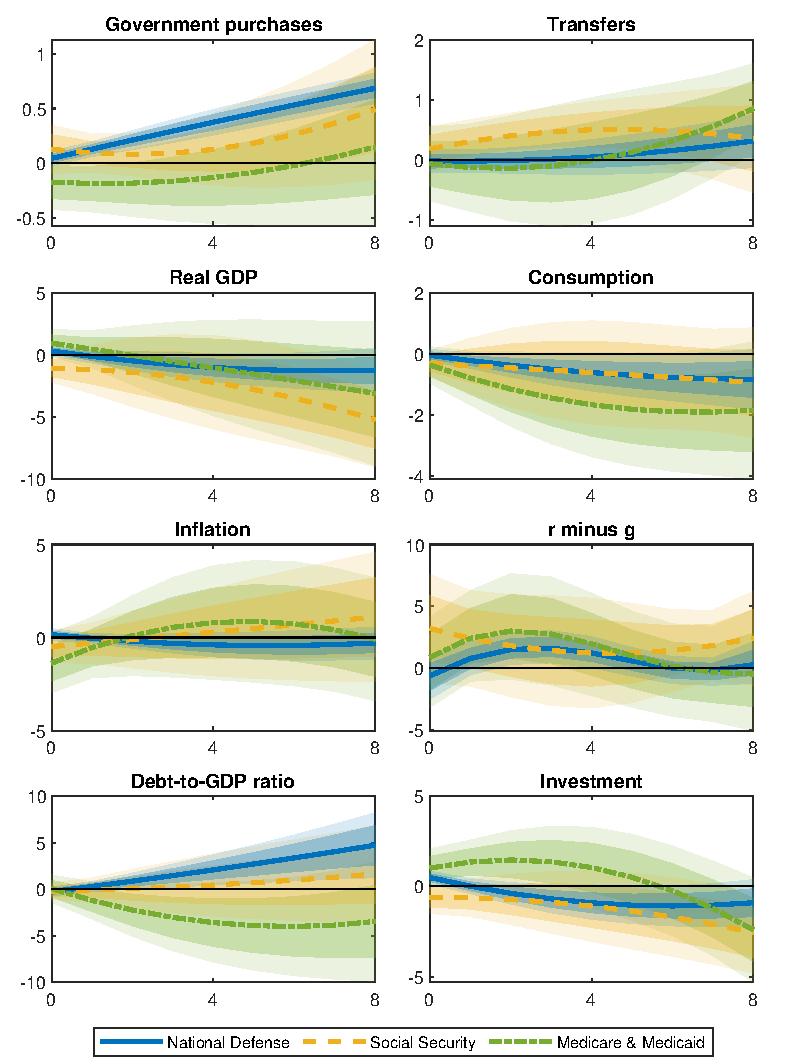
\includegraphics[trim=00mm 00mm 00mm 00mm, clip,width=0.495\textwidth]{figures and tables/figure_3DB.pdf}
    \caption{\textbf{Effects of anticipated spending shocks by category: Medicare \& Medicaid, Social Security, and National Defense.}
\\[0.5ex]
\small
Blue lines: responses to an anticipated shock to  National Defense. Yellow lines: responses to an anticipated shock to Social Security. Green lines: responses to an anticipated shock to Medicare \& Medicaid. The set of controls always includes four lags of the shock, output, and the outcome variable, plus four lags of transfers for panel Medicare \& Medicaid and Social Security, or four lags of government purchases for National Defense.  Each panel reports impulse responses from linear local projections estimated over the sample 1968q1-2019q4. Shaded areas: 68\% (dark) and 90\% (light) confidence bands.}  
    %\caption{\textbf{Effects of anticipated spending shocks by category -- Medicare \& Medicaid, Social Security, and National Defense over the full sample (1968q1–2019q4)}
%Impulse responses to anticipated government spending shocks across three major categories: Medicare \& Medicaid (green), Social Security (yellow), and National Defense (blue). The panels display the dynamic effects on key macroeconomic variables, including government purchases, transfers, output, consumption, inflation, the interest rate–growth differential (r – g), debt-to-GDP ratio, and investment. Shaded areas represent confidence bands.}
    \label{fig: SS DEF}
\end{figure}  

These responses do not condition on the fiscal backing of each category.
In what follows, we condition each category on its own measure of fiscal strain, described in Section \ref{sec:actuarial_soundeness}, and compare the resulting responses with the predictions of the model in Section \ref{sec:model}. Appendix \ref{sec: mand-disc} shows that the results extend to the aggregate categories of mandatory and discretionary spending.


\paragraph{Social Security.} Figure \ref{fig:SS OASIDI 8} presents impulse responses to an anticipated shock to Social Security spending for the period 1968q1-2019q4. Similar to Medicare and Medicaid, Social Security spending primarily consists of transfers to individuals; hence, each local projection includes four lags of transfers, as well as four lags each of the shock, output, and the outcome variable. 


The red (blue) lines indicate post-1974 (pre-1974) period when, as Figure \ref{fig:state_OASDI_actuarial_75y} shows, the OASDI trust funds are projected to be insolvent (solvent). 
The transmission of news shocks to SS spending differs sharply across the two regimes: when Social Security funding is expected to be ample, anticipated increases in spending appear to be more inflationary, and the response of real variables---GDP, consumption and investment---expansionary.
 
\begin{figure}[t!]
    \centering
    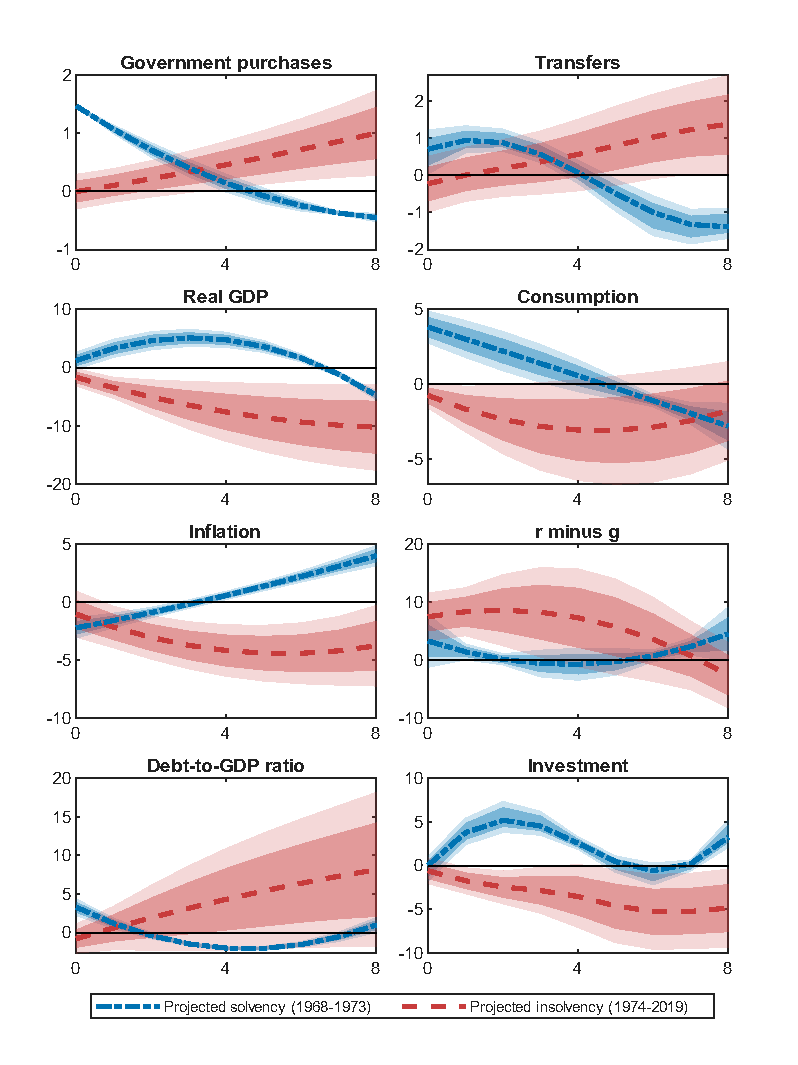
\includegraphics[trim=00mm 00mm 00mm 00mm, clip,width=0.495\textwidth]{figures and tables/figure_IRF_SS_actuarial_balance_newlabel.pdf}
    \caption{\textbf{Impulse responses to anticipated shocks to Social Security, conditional on OASDI actuarial balance.}
\\[0.5ex]
\small
%{\color{red} TO BE CORRECTED: Actuarial balance OASDI}\\
Impulse responses to anticipated shocks to Social Security (SS), conditional on the actuarial position of the OASDI trust funds. Red (blue) lines denote periods in which the system is actuarially unfunded (funded), based on the 75-year actuarial balance reported in the Trustees Reports. Estimates are obtained from state-dependent local projections over the sample 1968q1–2019q4. The set of controls always includes four lags of the shock, output, transfers, and the outcome variable.
Shaded areas: 68\% (dark) and 90\% (light) confidence bands.}
         \label{fig:SS OASIDI 8}
\end{figure}

Because the solvency regime covers only a few years at the start of our sample, we examine which spending announcements drive the responses estimated in that regime.
Figure \ref{fig:state OASIDI and shocks} shows that the largest SS shocks in our sample occurred in the 1960s and early 1970s, when the actuarial balance was positive. 
During this period, President Lyndon Johnson launched the Great Society initiatives, an ambitious effort to expand social spending and entitlements over several years, culminating in the large benefit increases legislated between 1969 and 1972. The U.S. economy was growing rapidly, and a favorable demographic structure provided supportive conditions for increased government funding of social programs. Indeed, the OASI and DI trust funds were largely in surplus at the time, and Social Security was perceived as self-financing, with no future fiscal adjustment expected.\
%footnote{See Appendix D for analogous figures displaying anticipated shocks to Medicare \& Medicaid and ND.} 
Once the actuarial balance turns negative and future adjustment is anticipated, the effects of SS spending become muted, consistent with fiscal backing. Both patterns are in line with the paradox of solvency.


\begin{figure}[t!]
    \centering
    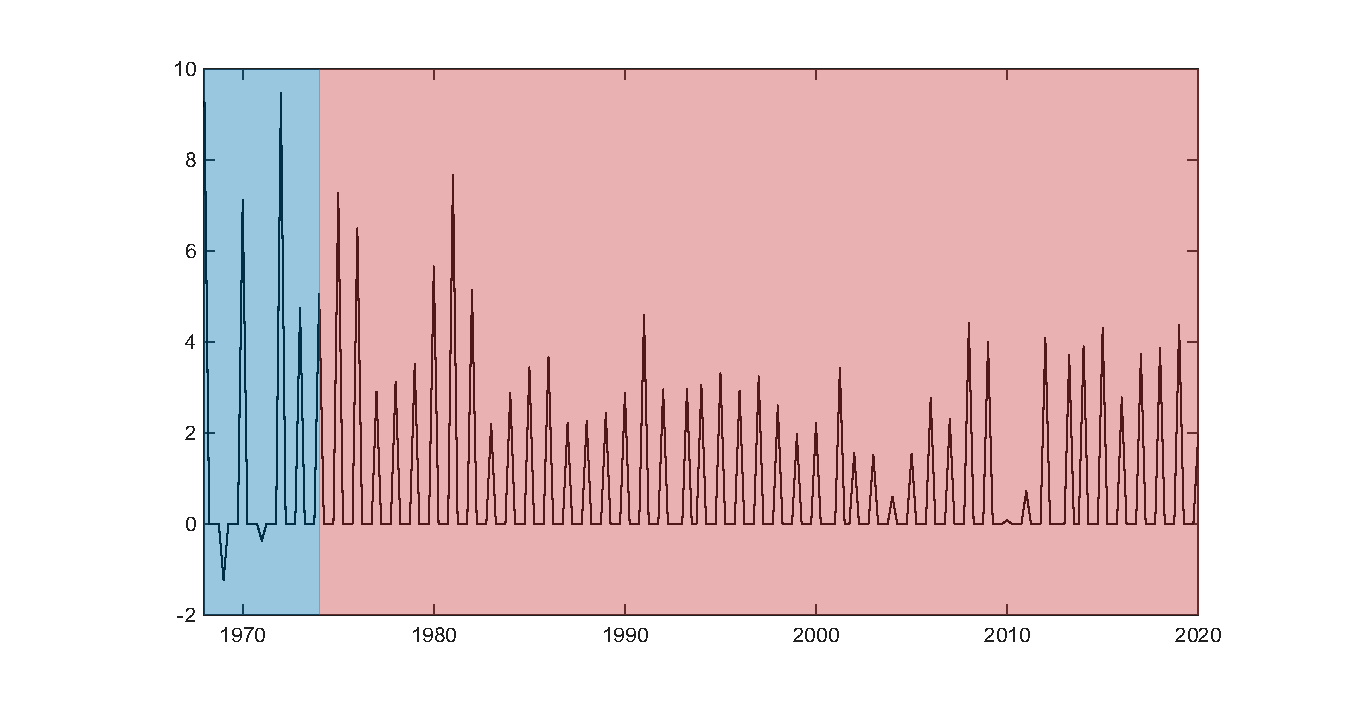
\includegraphics[trim=00mm 00mm 00mm 00mm, clip, scale=0.48]{figures and tables/f1q_state_oasdi75y.pdf}
\caption{\textbf{Anticipated shocks to Social Security and actuarial OASDI regimes.}
\\[0.5ex]
\small
%{\color{red} TO BE CHANGED: actaurial balance}\\
Black line: time series of anticipated shocks to Social Security, in percentage points. Shaded areas distinguish periods in which the OASDI system is actuarially funded (blue areas), when the 75-year actuarial balance is positive and no fiscal adjustment is expected, from periods in which it is actuarially unfunded (red areas), as described in Figure \ref{fig:state_OASDI_actuarial_75y}. Data on actuarial balances are drawn from the Trustees Reports.}
    \label{fig:state OASIDI and shocks}
\end{figure}


\paragraph{Medicare and Medicaid.} Because Medicare Parts B and D and Medicaid are automatically backed by general revenues, and the HI trust fund has been projected to be in deficit throughout our sample (see Figure \ref{fig:HI_actuarial}), the fiscal backing of MM does not vary over time. We therefore estimate linear local projections over 1968q1–2019q4, including four lags of transfers along with four lags of the shock, output, and the outcome variable.
\begin{figure}[t!]
     \centering
     \begin{subfigure}[b]{0.495\textwidth}
        \centering
        %\includegraphics[trim=00mm 00mm 00mm 00mm, clip,width=1\textwidth]{figures and tables/figure_6DBa.pdf}
        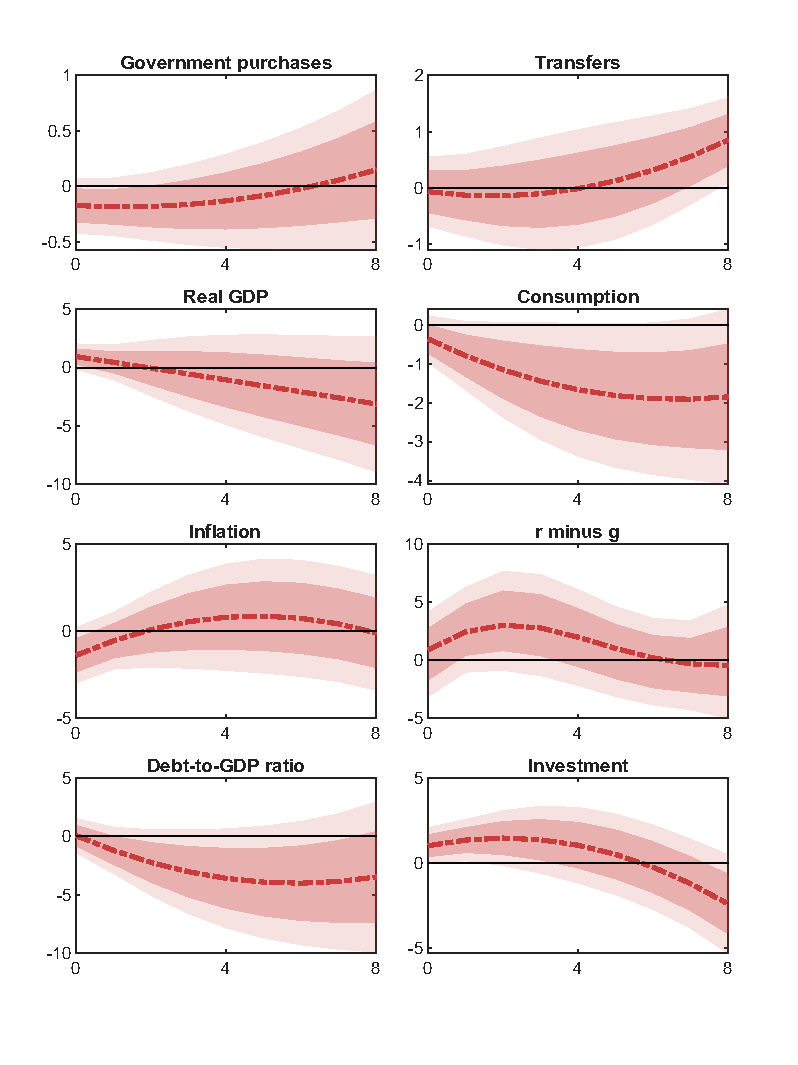
\includegraphics[trim=00mm 00mm 00mm 00mm, clip,width=1\textwidth]{figures and tables/figure_IRF_MM_6819_nostate.pdf}
        %\includegraphics[trim=10mm 50mm 10mm 50mm,clip,width=\textwidth]{figures and tables/MM HISMI 8.pdf}
         %\caption{Anticip. shock to MM, linear}
         %\label{fig:y equals x}
     \end{subfigure}
    
\caption{\textbf{Impulse responses to anticipated shocks to Medicare and Medicaid (MM).}
\\[0.5ex]
\small
Impulse responses to anticipated shocks to Medicare \& Medicaid (MM), estimated using linear local projections over 1968q1–2019q4. Controls include four lags of the shock, output, the outcome variable, and transfers. Shaded areas indicate 68\% and 90\% confidence bands.}
        \label{fig:MM}
\end{figure}
Figure \ref{fig:MM} displays a pattern consistent with fiscally backed spending. Transfers increase gradually and become statistically significant after a few periods, reflecting the anticipated nature of the shock and the delayed implementation of spending. Real GDP, and consumption decline following the announcement, while investment does so after some lags, indicating a contractionary effect during the anticipation period. At the same time, the interest rate–growth differential rises.
Inflation shows no persistent increase and remains broadly contained, further supporting the absence of wealth effects. Overall, these dynamics are consistent with Ricardian behavior, as agents anticipate that increases in MM spending will be offset by future fiscal adjustments.
These responses are stable over time and do not depend on fluctuations in fiscal capacity, as predicted by the model for programs that never enter the solvency region.




\begin{figure}[t!]
     \centering
         \begin{subfigure}[b]{0.495\textwidth}
           \centering
           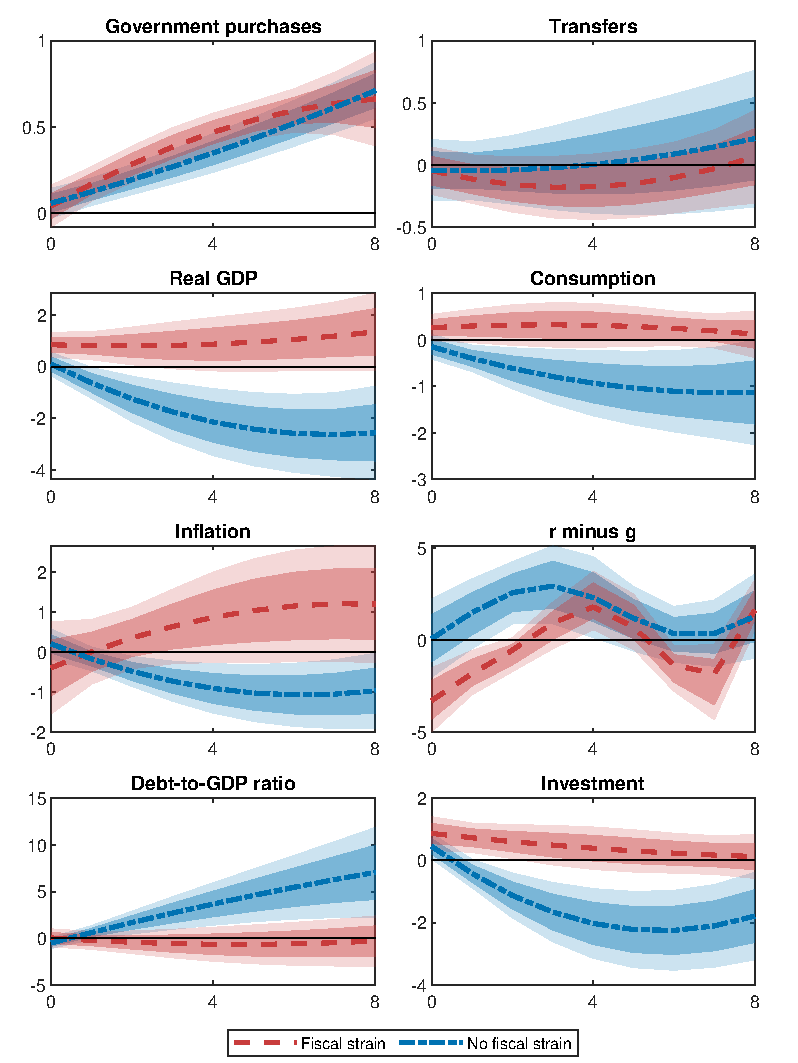
\includegraphics[trim=00mm 00mm 00mm 00mm, clip,width=1\textwidth]{figures and tables/figure_6DBb.pdf}
        %\includegraphics[trim=10mm 50mm 10mm 50mm, clip,width=\textwidth]{figures and tables/defense FI 8.pdf}
    %\caption{Anticip. shock to ND: FI}
     \end{subfigure}
\caption{\textbf{Impulse responses to anticipated shocks to National Defense (ND), conditional on fiscal capacity.} Red (blue) lines denote periods of fiscal strain (no fiscal strain) based on the Fiscal index (Figure \ref{fig:state FI}). Estimates are obtained from state-dependent local projections over 1968q1–2019q4. Controls include four lags of the shock, output, the outcome variable, and government purchases. Shaded areas indicate 68\% and 90\% confidence bands.}
%\\[0.5ex]
\small
        \label{fig:MM HISMI ND FI}
\end{figure}

\paragraph{National Defense.} Unlike mandatory programs, national defense has no dedicated account and no automatic access to general revenues: its fiscal backing depends on the residual fiscal space left after mandatory outlays. Following Figure \ref{fig:FDI_ND}, we condition on the Fiscal index, classifying 1969q1–1976q4 and 2009q1 onward as periods of scarce fiscal space. Results are robust to assigning fiscal strain to the post-2009 period only, when the index reached historically low levels and changes in the debt ceiling became more frequent (see Table \ref{table:debt_ceiling}).
Figure \ref{fig:MM HISMI ND FI} shows the results for state-dependent local projections, described by equation (\ref{eq:SDLP}), for an anticipated shock to National Defense spending in the period 1968q1-2019q4.
In this scenario, we include four lags of government purchases instead of transfers, and condition on the presence of slack (blue lines) or tightness (red lines) in the Fiscal index.
Our findings indicate a significant increase in government purchases under both fiscal states. On the other hand, the availability of resources to fund discretionary spending seems to play a crucial role in shaping the responses of real activity, inflation, and the debt-to-GDP ratio. Specifically, the responses of these variables are flipped in the two cases: when fiscal resources are abundant, the effects are muted and broadly consistent with Ricardian behavior; when resources are scarce, the shocks generate pronounced non-Ricardian effects. In the latter case, the anticipated increase in ND spending is more likely to be perceived as unbacked by future fiscal adjustment. This result aligns closely with theoretical predictions: Unfunded fiscal expansions are inflationary, stimulate economic activity and decrease the growth-interest rate differential, thus not worsening the debt-to-GDP ratio.\footnote{To complement this analysis, Appendix \ref{sec: mand-disc} extends the classification to a broader distinction between mandatory and discretionary spending, using the fiscal index to proxy the degree of fiscal strain across the two categories, as it reflects the residual resources available to discretionary spending after mandatory obligations are met. We confirm that mandatory spending shocks generally elicit Ricardian responses, irrespective of short-run fiscal strain, while discretionary shocks are more likely to generate non-Ricardian effects, particularly during periods of limited fiscal space.}
 
In Appendix \ref{app: sec: altern}, we assess the robustness of these findings across two distinct macroeconomic regimes. We split the sample in the Great Inflation and the ZLB period (1964q1-1979q2 and 2009q1-2015q4, respectively), and the Great Moderation years (1984q1-2008q4). The literature typically identifies the former as unbacked \textit{fiscal regimes} and the latter as a backed \textit{monetary regime}. We find that the effects of ND spending are Ricardian under the monetary regime and non-Ricardian under the fiscal regime.\footnote{These findings are consistent with those in \cite{ASCARI20231}, where the primarily focus is on defense spending shocks.} 
These patterns are consistent with the role of fiscal space discussed in Section \ref{sec:model}.


 
\paragraph{Warflation.} We now dig deeper into the inflationary effect of ND spending by focusing on specific historical episodes. This exercise should be read as a validation of the main mechanism we have discussed throughout the paper, namely, the distinction between Ricardian and non-Ricardian responses of ND spending, depending on the fiscal context. Rather than relying on regime indicators or fiscal indices, we now leverage the variation in defense outlays associated with historical U.S. war efforts. 

To this end, we adopt an alternative classification of states based on war periods.\footnote{While the previous analysis of defense spending was restricted to the 1968q1-2019q4 period, in what follows we extend the sample back to 1950q1 %-- the earliest date for which ND anticipated shocks are available.
This allows us to capture the onset of the Korean War and more accurately study the inflationary dynamics associated with major U.S. military conflicts.} War-related buildups in defense spending provide a natural experiment to test Ricardian versus non-Ricardian effects, as such spending is typically large and unexpected -- driven by external geopolitical needs.

  

We examine average annual ND spending as a percentage of GDP during each U.S. war period in our sample considering, when defense outlays remained elevated, even mobilization and demobilization quarters.
With this definition, average ND spending amounted to 13.4\% of GDP during the Korean War (1950Q2–1954Q3), 7.5\% during the Vietnam War (1964Q1–1975Q4), and 5.15\% during the Gulf War (1990Q1–1991Q4). From 2001 to 2011, during the Iraq and Afghanistan wars, defense spending averaged 4.1\%, and in the subsequent period 2011-2021, corresponding to the later years of the Afghanistan war, it averaged 3.4\%.

Based on the relative size of ND spending during different war periods, we consider yet another binary indicator variable, which takes the value of one during the periods corresponding to the three more expensive wars (i.e., Korean war, Vietnam war and Gulf war) and zero otherwise. This indicator is then used within the local projection framework of equation \eqref{eq:SDLP} to estimate state-dependent responses of inflation and other macroeconomic variables. 
We find (see Figure \ref{fig:defense wardates}) that outside these dates (highlighted in blue), impulse responses behave as Ricardian, whereas during high-cost war periods (in
red), they reflect a non-Ricardian pattern. 
Anticipated defense shocks lead to a sustained increase in government purchases in both states, with a  stronger response in periods of high war expenditure. In such episodes, defense spending significantly boosts GDP: output rises markedly and remains elevated, whereas it contracts during more ordinary times. Consumption and investment  fall in ordinary times, while these responses are not significant in periods of large war episodes.
%nvestment---although not statistically significant---performs better in war episodes, while it falls sharply otherwise.

Inflation also shows a clear divergence: it declines in ordinary circumstances but rises significantly when wars are costly, thereby reducing the interest–growth differential ($r-g$). This leads to very different debt dynamics: the debt-to-GDP ratio increases steadily in peacetime conditions, while it remains broadly stable, or even slightly declines, when fiscal pressures are driven by major wars.
These findings suggest that military spending shocks generate large multipliers and strong inflationary pressures, particularly during wartime. This historical episode analysis thus reinforces the main mechanism proposed in the paper: the fiscal context crucially conditions the macroeconomic effects of ND spending, with high-cost wartime periods displaying markedly non-Ricardian dynamics.

  
 \begin{figure}[t!]
    \centering
    %\includegraphics[trim=10mm 50mm 10mm 50mm,clip,width=\textwidth]{figures and tables/defense wardates 8.pdf}
    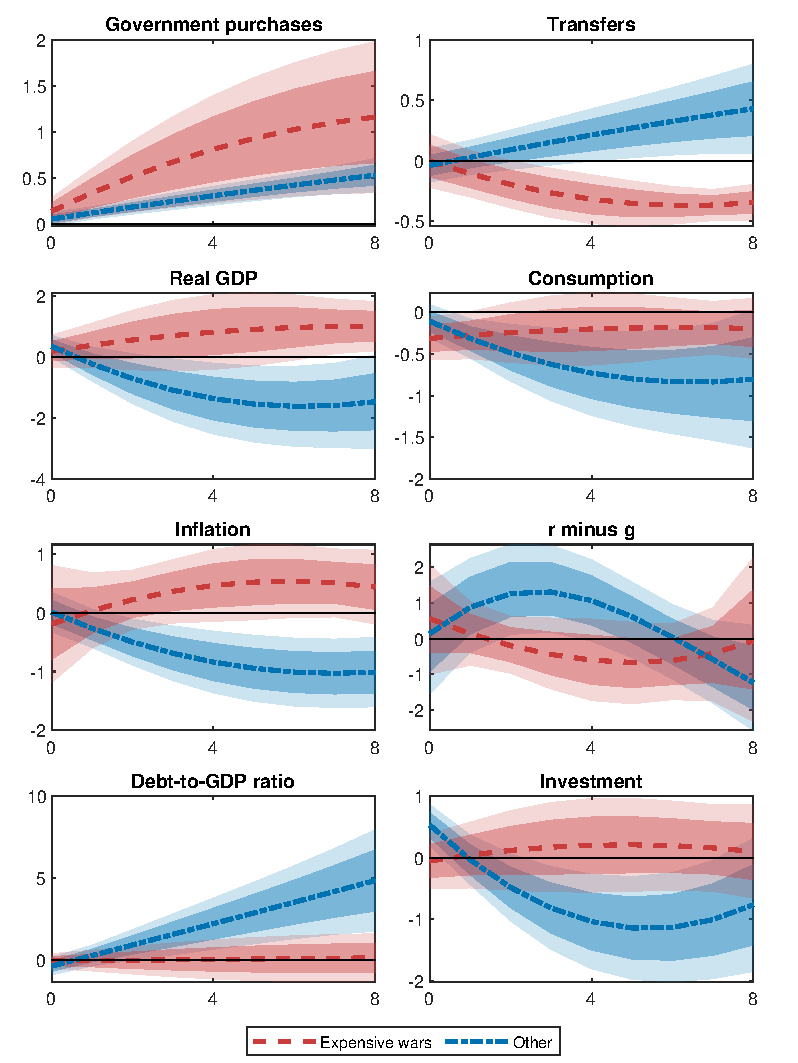
\includegraphics[trim=00mm 00mm 00mm 00mm, clip,width=0.495\textwidth]{figures and tables/figure_11_long6.pdf}
    %\includegraphics[trim=00mm 00mm 00mm 00mm, clip,width=0.495\textwidth]{figures and tables/figure_11DB.pdf}
    %\includegraphics[trim=00mm 00mm 00mm 00mm, clip,width=0.495\textwidth]{figures and tables/figure_11.pdf}
\caption{\textbf{Impulse responses to anticipated shocks to National Defense, distinguishing between high-cost war periods versus other periods.}
\\[0.5ex]
\small
Responses to an anticipated shock to National Defense, distinguishing between relatively more expensive war periods (red lines) and other times (blue lines).
We classify as high-cost war periods the Korean war (1950q2-1954q3) with average ND spending at 13.4\% of GDP, the Vietnam War (1964q1-1975q4) at 7.5\%, and the Gulf War (1990–1991), at 5.15\%. For reference, defense spending averaged 4.1\% of GDP during the Iraq War and the first years of the Afghanistan War (2001-2011), and 3.4\% of GDP in the subsequent years (2011-2021). 
Each panel reports impulse responses from state-dependent local projections estimated over the sample 1950q1-2019q4.
The set of controls always includes six lags of the shock, output, government purchases, and the outcome variable.
Shaded areas: 68\% (dark) and 90\% (light) confidence bands.
}
\label{fig:defense wardates}
\end{figure}  



\section{Conclusions}\label{sec: concl}
Fiscal policy is inherently complex, and not all government spending is alike in its macroeconomic impact. This paper argues that what matters is whether a spending expansion is fiscally funded, that is, whether the rules governing its financing generate credible expectations of future adjustment. Exploiting the program-specific funding rules established under U.S. law, we classify the fiscal backing of the main categories of federal spending ex ante, and test the resulting predictions on anticipated spending shocks constructed from U.S. Federal Budget projections.
A central implication of this approach is \textit{the paradox of solvency}. Programs financed through dedicated trust funds are subject to an asymmetric adjustment rule: corrective action is triggered when insolvency is projected, but no mechanism returns excess resources when the fund is expected to remain solvent. Such programs are therefore fiscally funded precisely when they are actuarially unfunded, and fiscally unfunded when they are actuarially funded. Social Security provides a natural test, as its actuarial position switched sign in 1974. Before then, when the system was perceived as self-financing, announced expansions—most notably those of the Great Society era and the large benefit increases of 1969–1972—generated inflationary and expansionary responses. After 1974, once trust-fund depletion became anticipated, the same announcements produced Ricardian responses. Medicare and Medicaid, which never entered the solvency region, generate Ricardian responses throughout the sample. Defense spending, which lacks a dedicated account and absorbs the residual fiscal space left by mandatory programs, displays pronounced non-Ricardian effects when that space is scarce, as during the costliest wars of the postwar period.

These findings suggest that the macroeconomic consequences of fiscal policy depend not only on the size and category of spending, but on the credibility of the mechanisms that back it. They also carry a lesson for the present. Projected trust-fund depletion does not by itself imply inflationary risk, as long as households expect sufficient corrective action. Conversely, if such action ceases to be credible—or if the priority of mandatory programs continues to erode the fiscal space available for discretionary spending—the inflationary footprint of fiscal policy may become larger.

%Fiscal policy is inherently complex, raising questions about whether different categories of spending in the U.S. Federal Budget have a larger impact on output and prices, and whether they have historically received varying levels of fiscal backing. Does the choice of fiscal tools matter to stimulate the economy during a recession? And, importantly, which spending categories pose a greater risk to price stability? This paper shows that not all spending is alike in its macroeconomic impact. 

%Shifts in discretionary spending, particularly in National Defense, display pronounced non-Ricardian effects, especially during times of limited or sharply reduced funding. In such contexts, insufficient fiscal resources can undermine the credibility of support for military expenditures, generating wealth effects that translate into higher output and inflation.

%By contrast, changes in mandatory spending, especially in Medicare and Medicaid, generally produce Ricardian effects, irrespective of funding pressures for these programs. %This pattern likely reflects the fact that these programs primarily finance healthcare services rather than direct income transfers, and are therefore perceived as being backed by default.
%Social Security spending presents a more nuanced case: large and sustained expansions of entitlements, such as those enacted during the Great Society era, have historically created expectations of permanent transfers, with meaningful upward pressure on prices.

%Overall, these findings suggest that the macroeconomic consequences of fiscal policy depend not only on the size and category of spending, but also on the credibility and persistence of its fiscal backing.

\singlespacing
\bibliographystyle{ecta}  
\bibliography{biblioafgm}

\appendix
\doublespace

 
\section*{Appendix}
\section{Data}

The outcomes of our local projections are quarterly data from NIPA tables of aggregate federal purchases \& investment, aggregate federal transfers, real GDP, real consumption, real investment, inflation, the interest rate-growth differential ($r-g$), and debt over GDP. All variables are expressed in levels. The interest rate-growth differential ($r-g$) is calculated as the difference between the nominal interest rate and the nominal GDP growth rate, both measured at quarterly frequency.

\paragraph{Trust funds for MM}

Medicare is funded through two main trust funds: The Hospital Insurance (HI) Trust Fund and Supplementary Medical Insurance (SMI) Trust Fund. The Hospital Insurance (HI) Trust Fund is primarily financed through payroll taxes collected under the Federal Insurance Contributions Act (FICA) for employees and employers, and under the Self-Employment Contributions Act (SECA) for self-employed individuals. Employees and employers each contribute a fraction of their wages, while high-income earners pay an additional Medicare surtax. The HI Trust Fund faces solvency challenges, and its balance depends on the balance of incoming payroll taxes and outgoing Medicare Part A expenses. The SMI Fund is primarily funded by general tax revenues and monthly premiums paid by Medicare enrollees and is primarily funded by general tax revenues and monthly premiums paid by Medicare enrollees; general-revenue transfers are determined automatically by law to match projected expenditures.
\paragraph{Trust funds for SS}
The Social Security Act mandates that Social Security spending be primarily financed through payroll taxes collected under the Federal Insurance Contributions Act (FICA). The OASI Trust Fund finances benefits for retirees and their survivors. It is primarily supported by payroll taxes levied on employees and employers, with a portion of earnings subject to these taxes capped at a specific threshold. The funds collected are used to pay monthly benefits to eligible retirees and to the survivors of deceased workers. The Disability Insurance (DI) Trust Fund provides benefits to individuals who become disabled and can no longer work. Like the OASI Trust Fund, the DI Trust Fund is also funded through payroll taxes. However, the DI Trust Fund has faced challenges in recent years due to increasing claims and demographic shifts, raising concerns about the sustainability of its funding.

General-revenue programs. The SMI trust fund is designed to remain solvent at all times, which distinguishes it fundamentally from the OASI, DI, and HI trust funds. Medicaid is financed through open-ended federal matching payments: the federal government is legally obligated to finance its share of eligible outlays through general revenues, according to the Federal Medical Assistance Percentage (FMAP). Because these programs continue to be fully financed when fiscal resources become scarce, they generate direct spillovers to the rest of the federal budget, shifting the burden of adjustment to programs without automatic revenue backing—most notably discretionary spending such as national defense, education, and infrastructure.

Investment of trust-fund surpluses. When the OASI, DI, and HI trust funds run surpluses, the federal government does not retain these resources as idle cash: a legally mandated investment and transfer mechanism is triggered. Surpluses are invested in special-issue Treasury bonds and certificates of indebtedness that are not available to the general public. These securities are backed by the full faith and credit of the United States, making them effectively risk free, and pay an interest rate tied to the average market yield on outstanding marketable Treasury obligations. The corresponding cash enters the General Fund and finances other federal expenditures, including defense, education, infrastructure, and the servicing of publicly held debt. Should trust-fund assets be exhausted, benefit payments would be constrained by incoming revenues, a scenario that creates strong political incentives for corrective legislation.
\paragraph{Periods of fiscal strain}
To assess the availability of funds for Medicare \& Medicaid and Social Security, we use their projected actuarial balances. These are obtained, respectively, from the Annual Report of the Boards of Trustees of the Federal Hospital Insurance and Federal Supplementary Medical Insurance Trust Funds and the Annual Report of the Board of Trustees of the Federal Old-Age and Survivors Insurance and Federal Disability Insurance Trust Funds, both available on the Social Security Administration website (https://www.ssa.gov/OACT/tr/
). For a detailed overview of the current financial status of both Social Security and Medicare trust funds, see Table 13.1, Cash Income, Outgo, and Balances of the Social Security and Medicare Trust Funds: 1936–2028, in the U.S. Budget.

%\begin{figure}[t!]
  %  \centering
  %  \includegraphics[trim=00mm 00mm 00mm 00mm, clip, scale=0.5]{figures and tables/state_comparison.pdf}
  %  \label{fig:state_comparison}
%\caption{\textbf{Comparison of periods implied by alternative fiscal capacity indicators.}
%\\[0.5ex]
%\small
%The figure contrasts the periods of high and low fiscal capacity identified by alternative indicators, serving as a basis for state-dependent analysis.
%Red areas: periods of fiscal strain.
%Blue areas: periods of absence of fiscal strain.}
%\end{figure}


% DONE-ALE: inserire il grafico con il confronto degli stati senza ALL
% DONE-ALE: cambiare colori alle figure
% DONE-ALE: controllare la figura 12, bande larghe e piccole.
% Purtoppo è un effetto del rescaling, dovuto al fatto che Mandatory spending non riesce a fare salire i transfers in questa figura
% DONE-ALE: scrivere le robe del moltiplicatore
% TO-DO-ALE: controllare la sezione Appendix A Data
% DONE-ALE: aggiustare figura 17 e 18
% DONE-ALE: nella sezione D, mettere le due figure con gli shock come la figura 9 nel testo. 
% - 5b ND shocks
% - 4 con MM shocks

\section{Mandatory and Discretionary spending}\label{sec: mand-disc}
%\subsubsection{Results for the linear case}
Does the variation in behavior across states appear only when examining specific subcategories of expenditure, or is it also evident in broader, aggregated categories like mandatory or discretionary spending?
We divide government expenditure into its two main components -- mandatory and discretionary -- and examine the impulse responses following an anticipated shock to each, using the longest time span covered by the data (1964q1-2019q4). The specification includes four lags of the control variables, namely the outcome variable, output, and both transfers and public purchases for mandatory expenditures and only public purchases for discretionary spending. We begin by estimating a linear model, as in equation (\ref{eq:linearLP}). As Figure \ref{fig:mand discr 64-19} shows, there are no marked differences in the responses of the variables between the two types of spending.

\begin{figure}[t!]
    \centering
    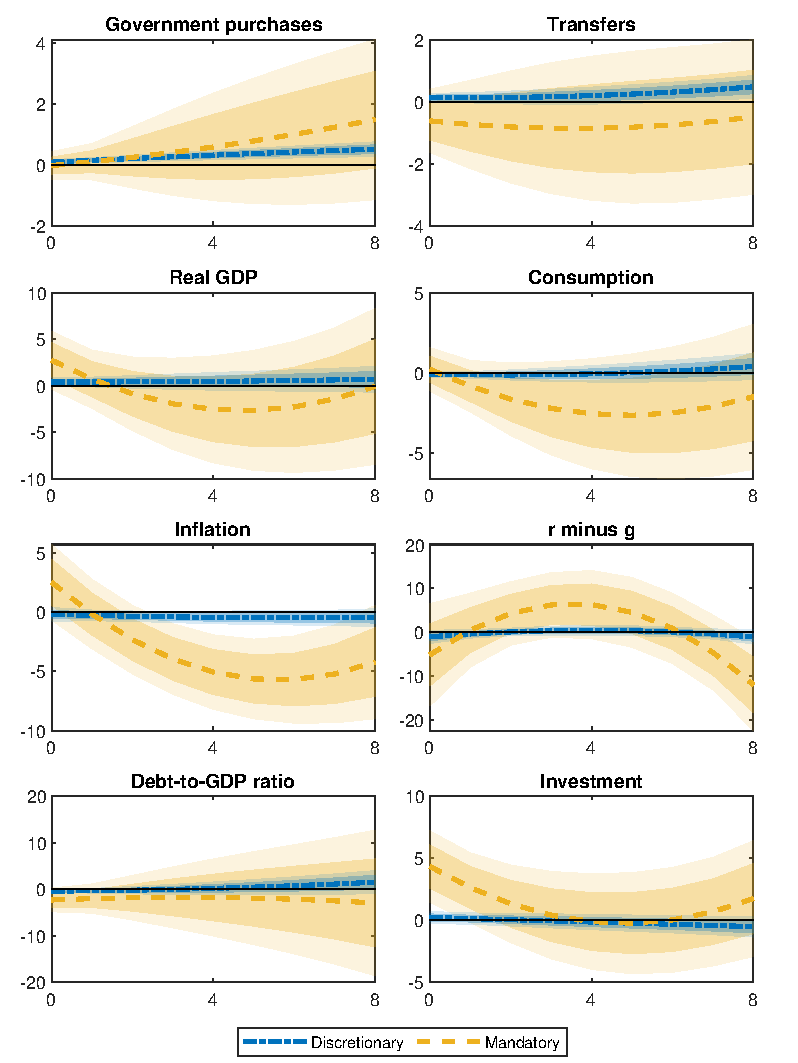
\includegraphics[trim=00mm 00mm 00mm 00mm, clip,width=0.495\textwidth]{figures and tables/figure_12DB.pdf}
    %\includegraphics[trim=10mm 50mm 10mm 50mm, clip,width=\textwidth]{figures and tables/mand discr 64-19.pdf}
    %\includegraphics[trim=10mm 70mm 10mm 50mm, clip,width=\textwidth]{figures and tables/mand discr 64-19 updated.pdf}
    \caption{\textbf{Effects of anticipated spending shocks to mandatory and discretionary spending.}
\\[0.5ex]
\small
Blue lines: responses to an anticipated shock to mandatory spending. Yellow lines: responses to an anticipated shock to discretionary spending. Each panel reports impulse responses from linear local projections estimated over the sample 1964q1-2019q4. The set of controls always includes four
lags of the shock, output, and the outcome variable, plus four lags of both transfers and government purchases for mandatory spending and only 
government purchases for discretionary spending. Shaded areas: 68\% (dark) and 90\% (light) confidence bands.
}
     \label{fig:mand discr 64-19}
\end{figure}

%We split the whole sample into two: 2001m1-2007m9 (regime M) and 2008m1-2017m12 (regime F). 
%\medskip
%\\The second sub-period is characterized by higher debt (see later). 


%\begin{frame}{\large{A look at their components: anticipated shock to SS and Defense} }

We employ the FI to distinguish a state with high fiscal capacity (where federal tax revenues exceed the amount required to cover mandatory expenses, with the surplus available to fund discretionary spending) (in red) from a state with a low capacity (in blue), using (\ref{eq:SDLP}).
Unlike in the linear case, mandatory and discretionary spending now exhibit different behaviors. As shown in Figure \ref{fig:mand discr FI}, the impulse response functions for mandatory spending consistently follow the pattern of a \textit{funded} spending shock. In contrast, impulse responses for discretionary spending behave like those following \textit{ funded} shocks when the FI is high but resemble \textit{unfunded} shocks when the FI is low, most evidently with respect to the response of output and consumption. 

\begin{figure}[t!]
     \centering
     \begin{subfigure}[b]{0.495\textwidth}
         \centering
        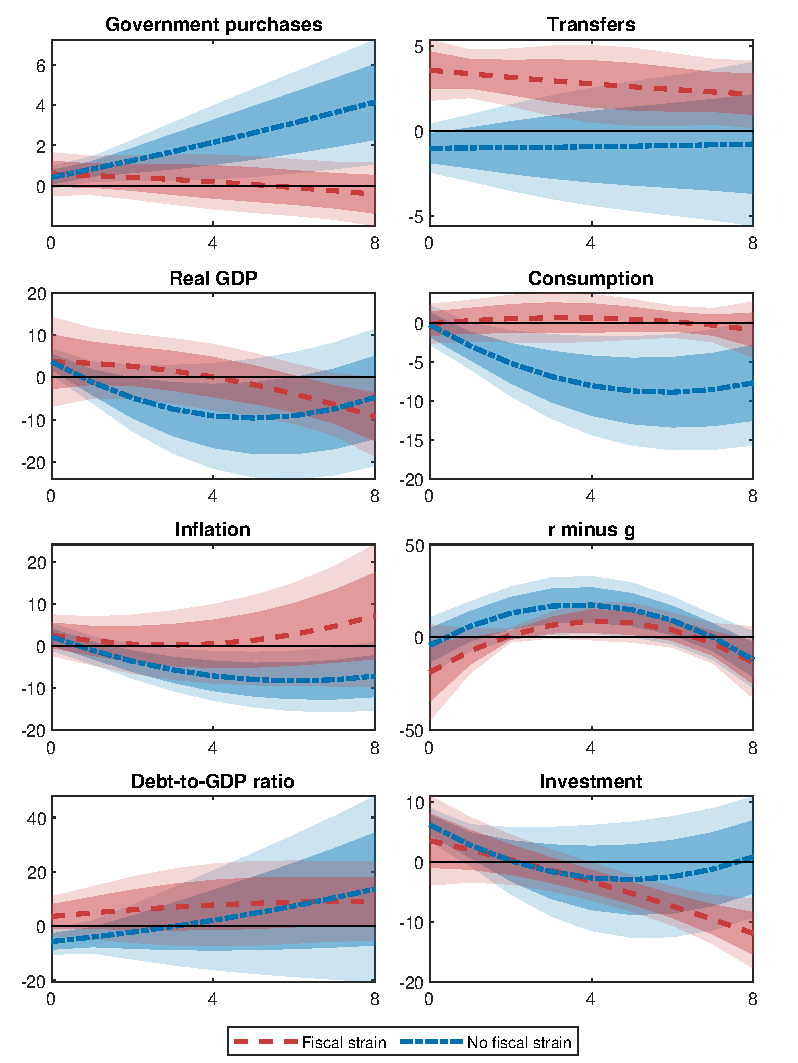
\includegraphics[trim=00mm 00mm 00mm 00mm, clip,width=1\textwidth]{figures and tables/figure_13DBa.pdf}
        %\includegraphics[trim=10mm 50mm 10mm 50mm,clip,width=\textwidth]{figures and tables/mandatory FI 8.pdf}
         \caption{Anticip. shock to mandatory, FI.}
         %\label{fig:y equals x}
     \end{subfigure}
     \hfill
     \begin{subfigure}[b]{0.495\textwidth}
         \centering
        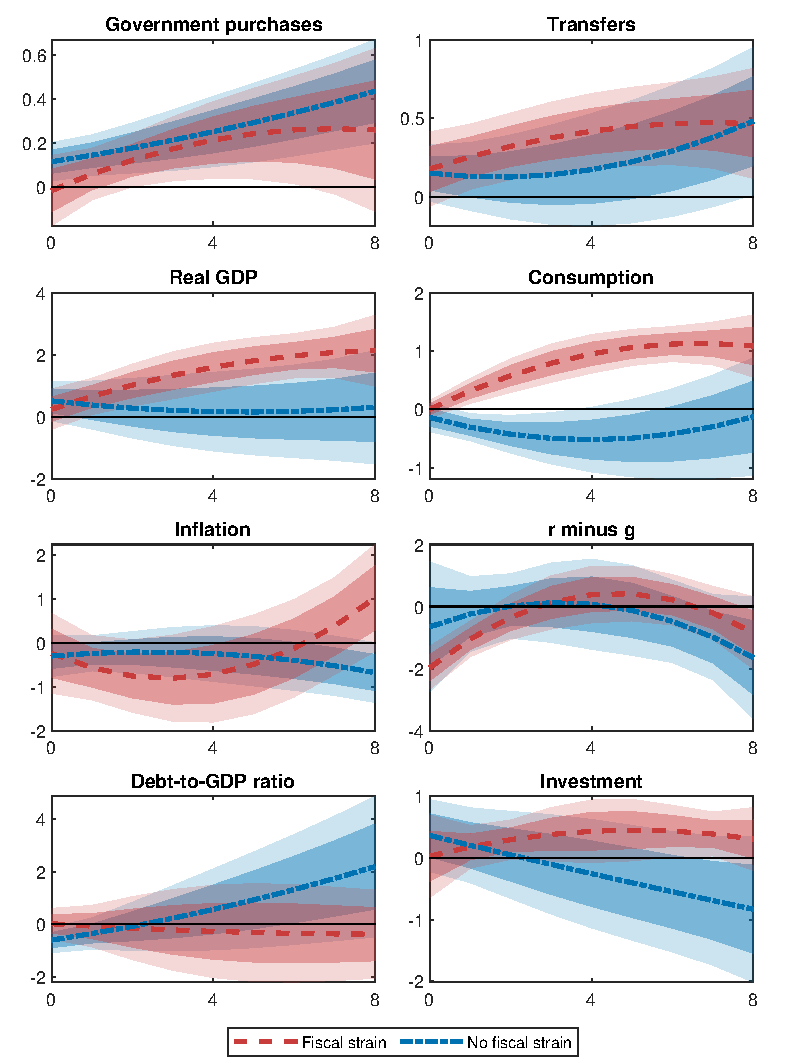
\includegraphics[trim=00mm 00mm 00mm 00mm, clip,width=1\textwidth]{figures and tables/figure_13DBb.pdf}         %\includegraphics[trim=10mm 50mm 10mm 50mm,clip,width=\textwidth]{figures and tables/discretionary FI 8.pdf}
         \caption{Anticip. shock to discretionary, FI}
         %\label{fig:three sin x}
     \end{subfigure}
        \caption{\textbf{Impulse responses to anticipated shocks to mandatory and discretionary spending, conditional on the Fiscal index.} 
\\[0.5ex]
\small
Panel (a): responses to anticipated shocks to mandatory spending. Panel (b): Responses to anticipated shocks to discretionary spending. 
Each panel reports impulse responses from state-dependent local projections estimated over the sample 1964q1-2019q4. Responses are conditioned on the periods of fiscal strain (red lines) or absence of fiscal strain (blue lines) in the Fiscal index, as described in Figure \ref{fig:state FI}. The set of controls always includes four lags of the shock, output, and the outcome variable plus four lags of both transfers and government purchases for panel (a) and only government purchases for panel (b). Shaded areas: 68\% (dark) and 90\% (light) confidence bands.}
\label{fig:mand discr FI}
\end{figure}
  
 %mandatory spending, largely composed of entitlement spending, requires the government to provide benefits without additional legislative action so.
The result for mandatory spending is not surprising. PAYGO, applied to mandatory spending to control deficit increases, requires that any rise in direct spending or revenue decrease must be offset by other spending cuts or revenue increases.\footnote{PAYGO, introduced in 1990 to curb deficits, was waived in the late 1990s due to surpluses and abandoned in 2002 after deficit-financed tax cuts. It was reinstated in 2007 and codified in the 2010 Statutory PAYGO Act, which mandates that new deficit-increasing legislation be offset or trigger automatic spending cuts (sequestration). Social Security and Medicaid are exempt, while Medicare can be reduced by up to 4\%. } These mechanisms ensure that such expenditures are consistently funded. Notably, PAYGO does not apply to discretionary spending, which is instead subject to annual budget caps and the appropriations process.
Overall, the behavior of mandatory and discretionary spending mirrors the results we obtained for their respective sub-components, respectively, MM that is always funded, and ND whose financing depends on fiscal capacity.\footnote{Note that while the distinction in behavior between high and low FI states is neat for ND, it becomes less so when looking at discretionary spending. This is likely because discretionary spending is an aggregate that encompasses various subcategories, whose behavior may not be as clear-cut as that of ND.}


% We now aim to examine whether the responses to anticipated shocks in mandatory and discretionary spending differ from what we have just observed when considering a scenario involving a less severe shortage of funds. Specifically, we focus on a case where there is a temporary deficit in the funds financing SS, rather than a full shortfall in the tax capacity to cover discretionary spending. To this end, we use the OASIDI index that we previously employed to study SS.\footnote{Results are unchanged if we use HISMI index for MM.}
% Results are in Figure \ref{fig:Discr Mand OASIDI}. Now both mandatory and discretionary spending behave as if always fully funded. This suggests that unbacked fiscal policies appear
% contingent on both time and government spending domains. In other words, temporary deficits in OASIDI funds may not be sufficient to make discretionary spending unfunded.

% \begin{figure}[t!]
%      \centering
%      \begin{subfigure}[b]{0.48\textwidth}
%          \centering
%         \includegraphics[trim=10mm 50mm 10mm 50mm,clip,width=\textwidth]{figures and tables/mandatory OASIDI 8.pdf}
%          \caption{Ant. shock to mandatory, OASIDI}
%          %\label{fig:y equals x}
%      \end{subfigure}
%      \hfill
%      \begin{subfigure}[b]{0.48\textwidth}
%          \centering
%          \includegraphics[trim=10mm 50mm 10mm 50mm,clip,width=\textwidth]{figures and tables/discretionary OASIDI 8.pdf}
%          \caption{Ant. shock to discretionary, OASIDI}
%          %\label{fig:three sin x}
%      \end{subfigure}
%         \caption{Anticipated shocks to mandatory and discretionary speding under OASIDI. In blue (red) regimes with fiscal strain (no fiscal strain).}
%         \label{fig:Discr Mand OASIDI}
% \end{figure}


 \section{Evidence with alternative states \label{app: sec: altern}}
\subsection{The Monetary-Fiscal regime (MF)}
Instead of relying on the previously fiscal Index, we now turn to a different approach to capture episodes of fiscal strain. Specifically, we now exploit the well-known distinction between a monetary-led regime (regime M) and a fiscally-led regime (regime F) found in the literature on monetary-fiscal interactions \citep[see][]{Bianchi2012,Bianchiillut, BM2014,BM2017,Chung2007}.\footnote{According to \cite{Leeper1991}, the monetary regime assumes an active monetary policy, adhering to the Taylor principle, and a passive fiscal policy. In this regime, fiscal expansions are always backed by future fiscal surpluses. Conversely, the fiscal regime assumes a passive monetary policy and an active fiscal policy: here, fiscal expansions are unbacked and generate wealth effects.} 

We assign a value of one to the unfunded fiscal sub-periods: the Great Inflation years (1964q1-1979q2) and the periods when monetary policy operated at the zero lower bound (2009q1-2015q4), while we assign a value of zero to the funded monetary regime: the Great Moderation years (1984q1-2008q4).\footnote{While there is a broad consensus on considering the Great Moderation as a monetary regime, the Great Inflation regime is more debated. Papers assuming a constantly passive fiscal policy detect, in the Great Inflation period, a double passive (hence, indeterminate) regime \citep[see][]{Lubik2004}). However, when allowing for a possible switch in fiscal policy, the pre-Volcker era is found to be consistent with a fiscally-led regime \citep[see][]{DavigLeeper2007,DL2011,sims2011}), in which the increasing inflation is attributed to a lack of fiscal discipline.} Blue (red) areas in Figure \ref{fig:state MF} identify a fiscal unfunded (monetary funded) regime. 


\begin{figure}[t!]
    \centering
    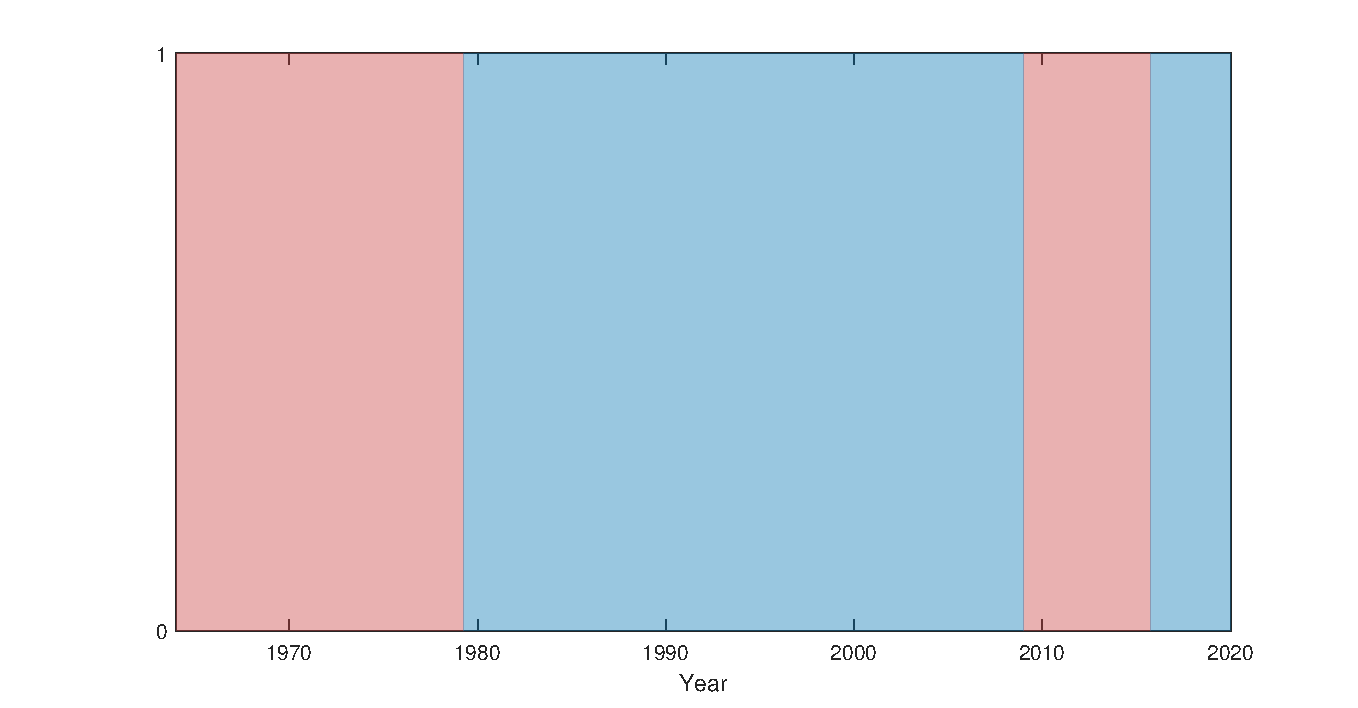
\includegraphics[trim=20mm 00mm 20mm 00mm, clip, scale=0.40]{figures and tables/state_MF.pdf}
    \caption{\textbf{Monetary and fiscal regimes.}
    \label{fig:states_MF}
\\[0.5ex]
\small
Periods of unfunded fiscal regime (in red) correspond to the Great Inflation years (1964q1-1979q2) and the years when monetary policy operated at the zero lower bound (2009q1-2015q4). Periods of funded monetary regime (in blue) correspond to the Great Moderation years (1984q1-2008q4).
}
    \label{fig:state MF}
\end{figure}

       
%\section{\textbf{A quantitative illustration using the \cite{SW} model}}
%\label{sec: SW} }
The decision to extend the fiscal regime beyond the Great Inflation years to the post-2009 period is motivated by several factors. Firstly, the post-2009 period is characterized by the zero lower bound (ZLB), indicating a passive monetary policy typical of a fiscal regime. Secondly, while pre-2009 changes in debt ceilings were relatively limited, in the post-2009 period, changes in debt ceilings were much more frequent, with different suspensions occurring. This implies that the ability to finance discretionary spending in general, and ND spending in particular, was subject to greater uncertainty and variability. Third, as \cite{BFM2023} stress, the amount of unfunded spending accelerates in the aftermath of the Great Recession. 

Given that this regime-based indicator is now used in place of the fiscal index, we reassess the baseline results presented in the paper. In particular, we evaluate how the responses to government spending shocks vary under this new specification -- both for defense spending and across the discretionary and mandatory components of government expenditures.
 Figure \ref{fig:defense MF} shows, for the sample 1964q1-2019q4, the responses of the variables to an anticipated shock to Defense spending under the fiscal regime (in blue) and under the monetary regime (in red).
Under regime M (F) output, consumption and investment decrease (increase), while the real rate and ($r-g$) increase (decrease) or are not significant. Inflation decreases (increases) under M (F), increasing (reducing) debt. Therefore, in regime M, the impulses behave as those following an anticipated funded spending shock; in regime F, the impulses
behave as those following an anticipated unfunded spending shock. The results we obtain employing the FI are therefore confirmed.


\begin{figure}[t]
    \centering
    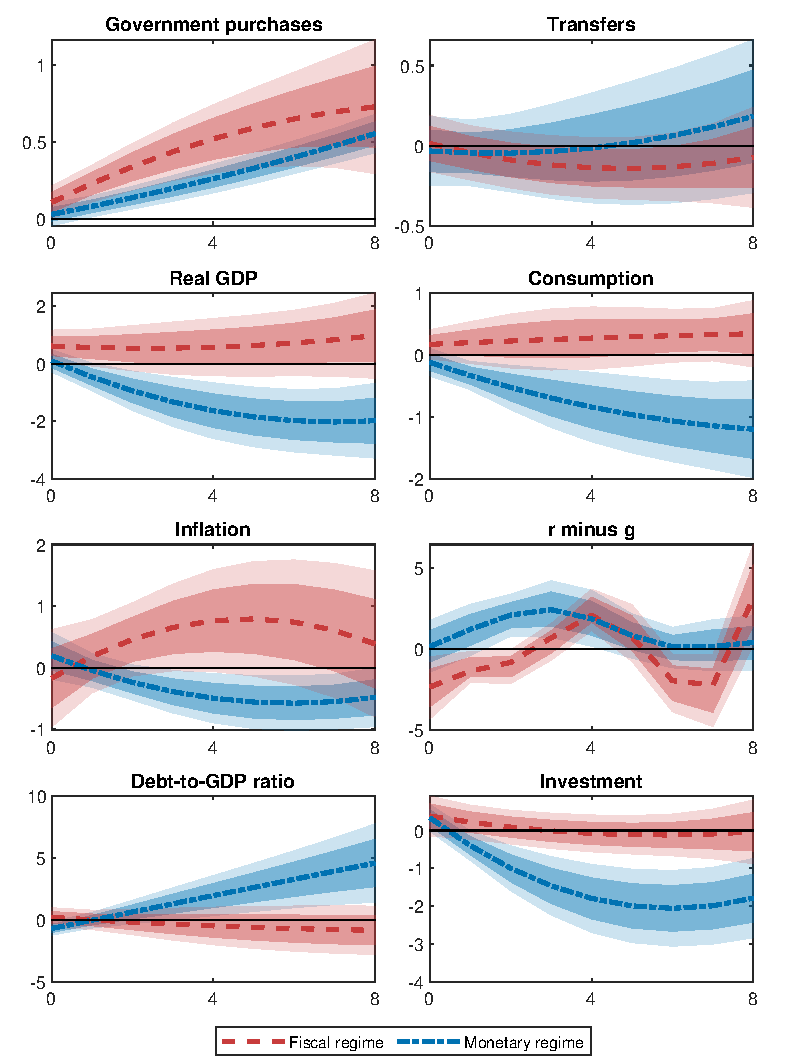
\includegraphics[trim=00mm 00mm 00mm 00mm, clip,width=0.495\textwidth]{figures and tables/figure_15DB.pdf}
    %\includegraphics[trim=00mm 00mm 00mm 00mm, clip,width=0.495\textwidth]{figures and tables/figure_15.pdf}
    %\includegraphics[trim=30mm 50mm 30mm 50mm, clip,width=\textwidth]{figures and tables/defense MF.pdf}
    \caption{\textbf{Impulse responses to anticipated shocks to National Defense, conditional
on monetary/fiscal regimes.}
\\[0.5ex]
\small
Responses to an anticipated shock to National Defense, conditioning on unfunded fiscal regimes (red lines) or funded monetary regimes (blue lines), as described in Figure \ref{fig:states_MF}.
Each panel reports impulse responses from state-dependent local projections estimated over the
sample 1964q1-2019q4. The set of controls always includes four lags of the shock, output, government purchases, and the outcome variable. Shaded areas: 68\% (dark) and 90\% (light) confidence bands.
}
    \label{fig:defense MF} 
\end{figure}

Looking at mandatory and discretionary spending across the MF states, we find that results under FI states are confirmed. As Figure \ref{fig:mand discr MF} shows, discretionary spending behaves as Ricardian under the Monetary regime and as non-Ricardian under the Fiscal regime. On the other hand, mandatory spending has always a 
Ricardian behavior both under the Monetary regime and under the Fiscal regime.

\begin{figure}[t]
     \centering
     \begin{subfigure}[b]{0.495\textwidth}
         \centering
        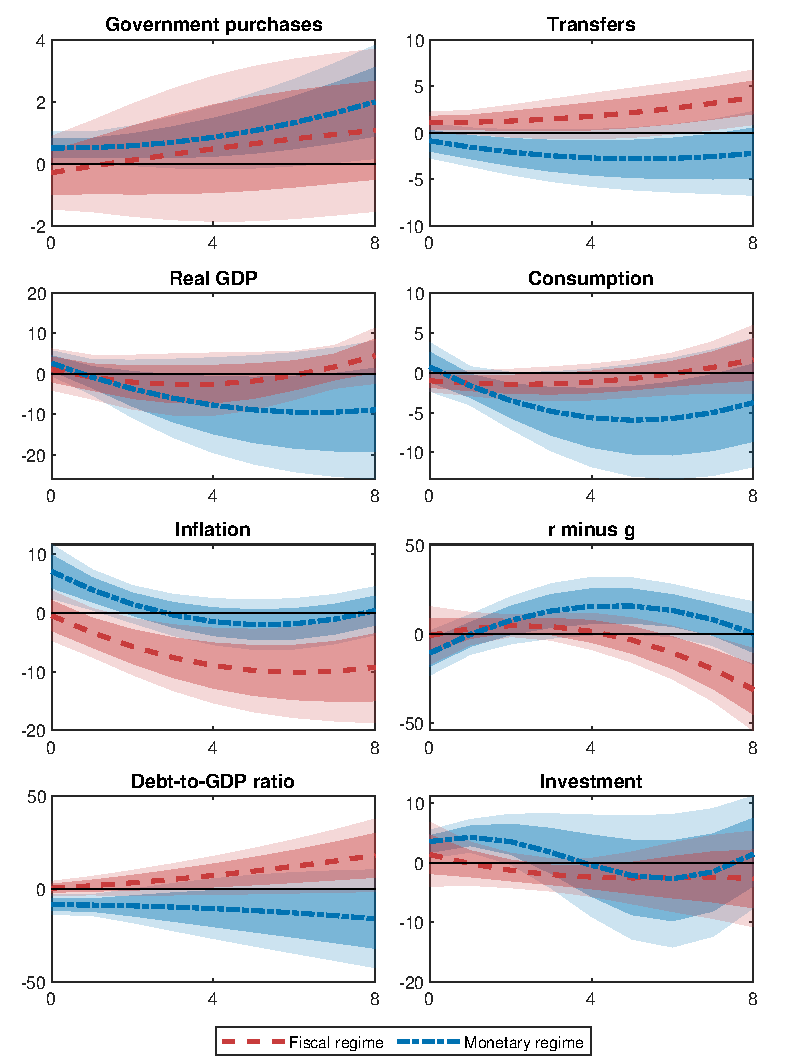
\includegraphics[trim=00mm 00mm 00mm 00mm, clip,width=1\textwidth]{figures and tables/figure_16DBa.pdf}
        %\includegraphics[trim=10mm 50mm 10mm 50mm,clip,width=\textwidth]{figures and tables/mandatory MF.pdf}
         \caption{Anticip. shock to mandatory, M/F regimes}
         %\label{fig:y equals x}
     \end{subfigure}
     \hfill
     \begin{subfigure}[b]{0.495\textwidth}
         \centering
         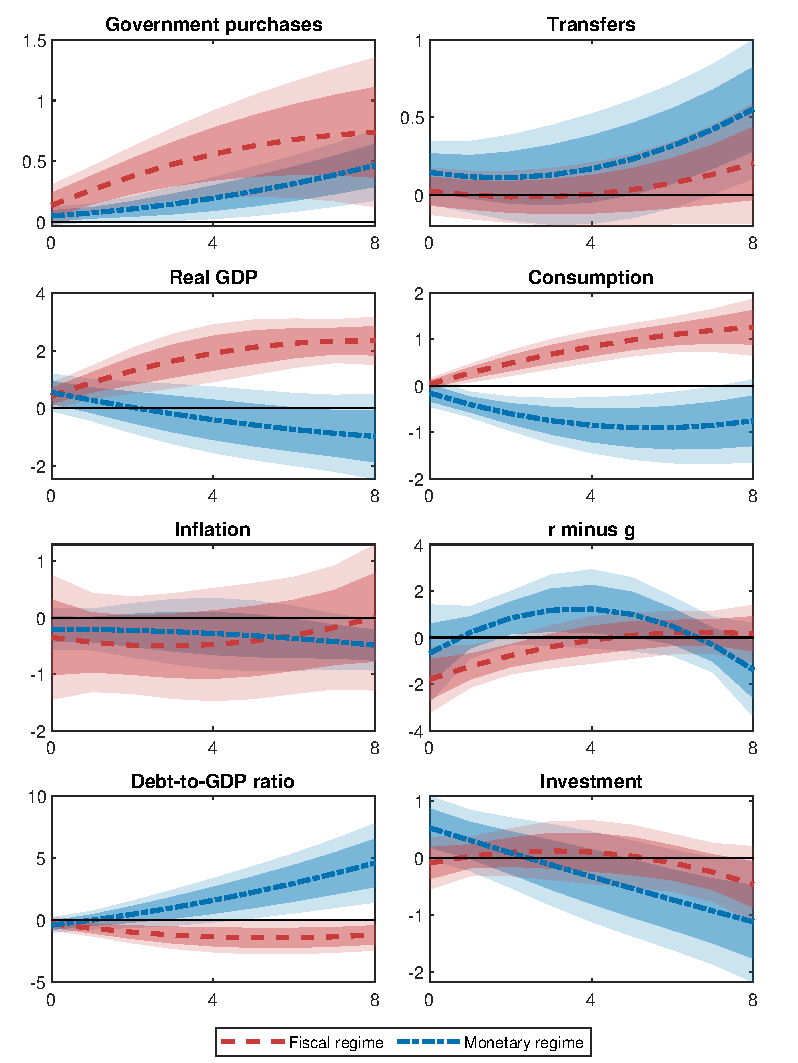
\includegraphics[trim=00mm 00mm 00mm 00mm, clip,width=1\textwidth]{figures and tables/figure_16DBb.pdf}
         %\includegraphics[trim=10mm 50mm 10mm 50mm,clip,width=\textwidth]{figures and tables/DISCR 64-19 MF.pdf}
         \caption{Anticip. shock to discretionary, M/F regimes}
         %\label{fig:three sin x}
     \end{subfigure}
    \caption{\textbf{Impulse responses to anticipated shocks to mandatory and discretionary spending, conditional on the monetary/fiscal regimes.} 
    \\[0.5ex]
    \small
    Panel (a): responses to anticipated shocks to mandatory spending. Panel (b): Responses to anticipated shocks to discretionary spending. 
    Each panel reports impulse responses from state-dependent local projections estimated over the sample 1964q1-2019q4. Responses are conditioned on the unfunded fiscal regimes (red lines) or funded monetary regimes (blue lines), as described in Figure 14. The set of controls always includes four lags of the shock, output, and the outcome variable plus four lags of both transfers and government purchases for panel (a) and only government purchases for panel (b). Shaded areas: 68\% (dark) and 90\% (light) confidence bands.}
    \label{fig:mand discr MF}
\end{figure}

%When we look at how the sub-components of Mandatotry spending, namely SS and MM, behave under MF states we get Figure \ref{fig:SS MM MF}. 


%\begin{figure}[t!]
   %  \centering
    % \begin{subfigure}[b]{0.48\textwidth}
      %   \centering
       % \includegraphics[trim=10mm 50mm 10mm 50mm,clip,width=\textwidth]{figures and tables/SS MF.pdf}
       %  \caption{Ant. shock to SS, MF}
         %\label{fig:y equals x}
     %\end{subfigure}
   %  \hfill
   %  \begin{subfigure}[b]{0.48\textwidth}
      %   \centering
        % \includegraphics[trim=10mm 50mm 10mm 50mm,clip,width=\textwidth]{figures and tables/other mandatory MF no g.pdf}
        % \caption{Ant, shock to MM, MF}
         %\label{fig:three sin x}
    % \end{subfigure}
       % \caption{Anticipated shocks to discretionary and mandatory spending under MF states}
       % \label{fig:SS MM MF}
%\end{figure}

%As in the case with FI states, we get that SS behaves as funded in M and as almost funded in F. MM, except for investment,
%always behave as funded. In other words, SS stays backed but with some difficulty.
%Exactly as with FI in the text, even employing MF states we get that while mandatory is always funded, the behavior of the subcomponents is blurred, as confirmed from the response to a shock to Other mandatories in Figure \ref{fig:othermand MF} that behave as \textit{almost funded} in M and \textit{almost unfunded} in F. 
  

 %\begin{figure}[t!]
 %   \centering
  %  \includegraphics[trim=10mm 50mm 10mm 50mm, clip,width=\textwidth]{figures and tables/other mandatory MF no g.pdf}
  %  \caption{ Ant. shock to Othermand, MF}
  %  \label{fig:othermand MF} 
%\end{figure}


%\paragraph{Summary for MF states \label{app: sec: summ mf} }

%\begin{itemize} 
%\item discretionary: as \textit{funded} (\textit{unfunded}) when the FI is high (low).
% \item[$\to$] Defense: as \textit{funded} (\textit{unfunded}) when the FI is high (low).
 %\item[$\to$] Non-Defense: no clear path.
 %\item mandatory: always as \textit{funded}.
 %\item[$\to$] SS: as \textit{funded} (\textit{almost funded}) when the FI is high (low).
 %\item[$\to$] MM: always as \textit{funded}.
 %\item[$\to$] Othermandatory: as \textit{almost unfunded} (\textit{almost funded}) when the FI is high (low).
% \end{itemize}

% \subsection{Evaluating Social Security and Medicare \& Medicaid using the Fiscal index\label{app: sec: cross}}
% We now turn to examine the effects of anticipated shocks to Social Security and Medicare \& Medicaid conditioned on the Fiscal index.
 %and vice versa, that is evaluating ND using the states identified for SS and MM.
%  \paragraph{FI}
%  As a first exercise, we evaluate the effects of an anticipated shock to SS employing the FI.
% Figure \ref{fig:SS MM FI} shows the impulse responses to anticipated shocks for MM (panel (a)) and SS (panel (b)) in this case. The results for Medicare \& Medicaid display Ricardian behavior regardless of the fiscal strain, consistent with the findings shown in Figure \ref{fig:MM HISMI ND FI} (a). In contrast, the impulse responses for Social Security reveal that during periods of high fiscal strain indicated by the FI, anticipated increases in SS spending appear more inflationary.
 %This outcome contrasts with the evidence from Figure \ref{fig:SS OASIDI 8}, where anticipated SS shocks, conditioned on the OASDI trust funds' financial status, showed that increases in SS spending were more inflationary when the trust funds were in surplus (i.e., when fiscal backing was ample), and less so or insignificant during deficit periods. In other words, conditioning on SS's own fiscal capacity suggested that stronger fiscal backing amplified inflationary effects, whereas under the Fiscal index (which measures discretionary spending capacity), the largest inflationary effects arise during periods of overall fiscal strain. 
%The reason for this difference lies in the timing of large SS shocks: the most significant shocks from the 1960s and early 1970s occur during periods classified as high fiscal strain by the FI (depicted in blue).

 
  %As figure \ref{fig:SS FI wt big} shows, when the sample is restricted to start from 1975q1 -- thus excluding the large shocks from the 1960s and early 1970s -- the effects of SS spending revert to Ricardian behavior regardless of the fiscal strain regime. This result mirrors the earlier findings based on the program-specific fiscal capacity (Figure \ref{fig:SS OASIDI wt big}) and reinforces the idea that the inflationary impact of anticipated SS shocks is primarily driven by the expansive entitlement programs during the Great Society era.
 %: output, consumption, and investments either decrease or remain insignificant. ($r-g$) increase or is not significant. Inflation, even if it (insignificantly) increases in the low FI regime, does not significantly reduce debt. We can conclude that SS behaves as \textit{funded} when the FI is high and \textit{almost funded} when FI is low. The right panel of Figure \ref{fig:SS MM FI} reports results for MM that always behave as \textit{funded}.

  %\begin{figure}[t!]
      % \centering
      % \begin{subfigure}[b]{0.48\textwidth}
        %   \centering
        %\includegraphics[trim=00mm 00mm 00mm 00mm, clip,width=1\textwidth]{figures and tables/figure_18a.pdf}
          %\includegraphics[trim=10mm 50mm 10mm 50mm,clip,width=\textwidth]{figures and tables/MM fiscalindex.pdf}
         %  \caption{Ant. shock to MM, FI}
           %\label{fig:y equals x}
       %\end{subfigure}
      % \hfill
      % \begin{subfigure}[b]{0.48\textwidth}
           %\centering
           %\includegraphics[trim=00mm 00mm 00mm 00mm, clip,width=1\textwidth]{figures and tables/figure_18b.pdf}
            %\includegraphics[trim=10mm 50mm 10mm 50mm,clip,width=\textwidth]{figures and tables/SS fiscalindex.pdf}
           %\caption{Ant. shock to SS, FI}
           
%\label{fig:three sin x}
     %  \end{subfigure}
        % \caption{\textbf{Impulse responses to anticipated shocks to Medicare and Medicaid and Social Security conditional on the Fiscal index.}
%\\[0.5ex]
%\small
%Panel (a): responses to an anticipated shock to Medicare \& Medicaid. Panel (b): responses to an anticipated shock to Social Security. Both shocks are conditioned on the periods of fiscal strain (red lines) or absence of fiscal strain (blue lines) in the Fiscal index, as described in Figure \ref{fig:state FI}.
%Each panel reports impulse responses from state-dependent local projections estimated over the sample 1968q1-2019q4.
%The set of controls always includes four lags of the shock, output, and the outcome variable, plus four lags of transfers. 
%Shaded areas: 90\% confidence bands.}
 %       \label{fig:MM HISMI ND FI}
%\end{figure}


%\begin{figure}[t!]
 %   \centering
  %  \includegraphics[trim=00mm 00mm 00mm 00mm, clip,width=0.495\textwidth]{figures and tables/figure_19.pdf}
    %\includegraphics[trim=00mm 00mm 00mm 00mm, clip,width=0.495\textwidth]{figures and tables/SS FI from 1975.pdf}
%\caption{\textbf{Impulse responses to anticipated shocks to Social Security (SS), conditional on the Fiscal Index, over the subperiod 1975q1-2019q4.}
%\\[0.5ex]
%\small
%Responses to an anticipated shock to Social Security, conditioning on the periods of fiscal strain (red lines) or absence of fiscal strain (blue lines) in the Fiscal index, as described in Figure \ref{fig:state FI}.
%Each panel reports impulse responses from state-dependent local projections estimated over the sample 1975q1-2019q4.
%The set of controls always includes four lags of the shock, output, transfers, and the outcome variable.
%Shaded areas: 90\% confidence bands.
%}
 %   \label{fig:SS FI wt big}
%\end{figure}


%  Although mandatory always behaves as funded, the behavior of its sub-components is blurred, as confirmed by the impulse response functions following a shock to Other mandatory components in Figure \ref{fig:Othermand FI}.

% % \begin{figure}[t!]
%  %    \centering
%   %    \includegraphics[trim=10mm 50mm 10mm 50mm, clip,width=\textwidth]{figures and tables/othermand fiscalindex.pdf}
%    %  \caption{Ant. shock to Other mandatory: FI}
%     % \label{fig:Othermand FI}
%  %\end{figure}

%  \FloatBarrier
 
% % \paragraph{Summary for FI states\label{app: sec: summ fi} }


% % \begin{itemize} 
% % \item discretionary: as \textit{funded} (\textit{unfunded}) when the FI is high (low).
% %  \item[$\to$] Defense: as \textit{funded} (\textit{unfunded}) when the FI is high (low).
% %  \item[$\to$] Non-Defense: no clear path.
% %  \item mandatory: always as \textit{funded}.
% %  \item[$\to$] SS: as \textit{funded} (\textit{almost funded}) when the FI is high (low).
% %  \item[$\to$] MM: always as \textit{funded}.
% %  \item[$\to$] Othermandatory: as \textit{almost unfunded} (\textit{almost funded}) when the FI is high (low).
% %  \end{itemize}
% %  \paragraph{OASIDI}
%  The other check we propose is to assess Defense spending in the OASDI and HISMI states. As Figure \ref{fig:Defense OASIDI HISMI} shows, there is no clear difference in the responses of the variables between the two states. Furthermore, under OASIDI and HISMI, they behave as they would under a funded spending shock. A possible interpretation could be that periods when SS trust funds are in deficit are not times of generalized scarcity of funds to cover expenses, which are instead backed.

%  \begin{figure}[t!]
%       \centering
%       \begin{subfigure}[b]{0.48\textwidth}
%           \centering
%          \includegraphics[trim=10mm 50mm 10mm 50mm,clip,width=\textwidth]{figures and tables/DEFENSE oasidi.pdf}
%           \caption{Ant. shock to Defense, OASIDI}
%           %\label{fig:y equals x}
%       \end{subfigure}
%       \hfill
%       \begin{subfigure}[b]{0.48\textwidth}
%           \centering
%           \includegraphics[trim=10mm 50mm 10mm 50mm,clip,width=\textwidth]{figures and tables/defense under HISMI.pdf}
%           \caption{Ant. shock to Defense, HISMI}
%           %\label{fig:three sin x}
%      \end{subfigure}
%          \caption{TBA}
%          \label{fig:Defense OASIDI HISMI}
%  \end{figure}

%   As Figure \ref{fig:Discr Mand OASIDI} shows, we get the same results if we look at mandatory and discretionary spending in OASIDI states; i.r.f. behaving as under a \textit{funded} spending shock.\footnote{We get the same result if we look at HISMI states.} 
 
 
% % \paragraph{Summary for OASIDI (HISMI) states\label{app: sec: summ oasidi} }

% % \begin{itemize} 
% % \item discretionary: always as \textit{funded}.
% %  \item[$\to$] Defense: always as \textit{funded}.
% %  \item[$\to$] Non-Defense: no clear path.
% %  \item mandatory: always as \textit{funded}.
% %  \item[$\to$] SS: always as \textit{funded}.
% %  \item[$\to$] MM: always as \textit{funded}.
% %  \item[$\to$] Othermandatory: as \textit{unfunded} in surplus and as \textit{funded} in deficit. 
% %  \end{itemize}
% \subsection{Deficit in all trust funds states\label{app: sec: ALL} }

% We want to stress the robustness of the results by considering an alternative state. Specifically, we now want to see how the impulse responses to an anticipated shock to Social Security, Medicare and Medicaid and National Defense spending change when all the trust funds for both SS (OASDI) and Medicare/Medicaid (HISMI) are simultaneously in deficit. The sample period is 1968q1-2019q4. States are depicted in Figure \ref{fig:state ALL}: we assign a value of one (in blue) if both trust funds are in deficit, and 0 (in red) otherwise. The blue lines in the following figures depict the responses of the variables in the case of a joint deficit, while the red lines depict the responses in the case of a surplus.


% \begin{figure}[t!]
%     \centering
%     \includegraphics[trim=20mm 00mm 20mm 00mm, clip, scale=0.40]{figures and tables/state_ALL.pdf}
%     \caption{\textbf{Fiscal capacity when all the trust funds are in deficit.}
%     \\[0.5ex]
%     \small
%     Shaded areas reflect the joint status of the trust funds for both Social Security(OASDI funds) and Medicare \& Medicaid (HISMI funds): blue indicates periods of fiscal strain (both in deficit), red indicates periods without strain (at least one not in deficit).}
%     \label{fig:state ALL}
% \end{figure}

% %mandatory behaves as \textit{funded} in surplus and as \textit{unfunded} in deficit, the discretionary behave as \textit{funded}.


% %\begin{figure}[t!]
%    %  \centering
%     % \begin{subfigure}[b]{0.48\textwidth}
%       %   \centering
%       %  \includegraphics[trim=10mm 50mm 10mm 50mm,clip,width=\textwidth]{figures and tables/mandatory all states.pdf}
%         % \caption{Ant. shock to mandatory, ALL}
%          %\label{fig:y equals x}
%      %\end{subfigure}
%     % \hfill
%     % \begin{subfigure}[b]{0.48\textwidth}
%          %\centering
%         % \includegraphics[trim=10mm 50mm 10mm 50mm,clip,width=\textwidth]{figures and tables/discr ALL.pdf}
%         % \caption{Ant. shock to discretionary, ALL}
%          %\label{fig:three sin x}
%     % \end{subfigure}
%       %  \caption{Anticipated shocks to mandatory and discretionary spending under ALL states}
%        % \label{fig:Mand Disc ALL}
% %\end{figure}

 


% As Figure \ref{fig:SS MM ALL} shows, even with this regime specification, the responses for SS (on the left) and those for MM (on the right) are confirmed. 

% \begin{figure}[t!]
%      \centering
%      \begin{subfigure}[b]{0.495\textwidth}
%          \centering
%         \includegraphics[trim=00mm 00mm 00mm 00mm, clip,width=1\textwidth]{figures and tables/figure_18a.pdf}
%         %\includegraphics[trim=10mm 50mm 10mm 50mm,clip,width=\textwidth]{figures and tables/SS tutte.pdf}
%          \caption{Ant. shock to SS, overall deficit}
%          %\label{fig:y equals x}
%      \end{subfigure}
%      \hfill
%      \begin{subfigure}[b]{0.495\textwidth}
%          \centering
%         \includegraphics[trim=00mm 00mm 00mm 00mm, clip,width=1\textwidth]{figures and tables/figure_18b.pdf}         %\includegraphics[trim=10mm 50mm 10mm 50mm,clip,width=\textwidth]{figures and tables/MM ALL states.pdf}
%          \caption{Ant. shock to MM, overall deficit}
%          %\label{fig:three sin x}
%      \end{subfigure}
%         \caption{\textbf{Impulse responses to anticipated shocks to Social Security and Medicare and Medicaid, conditional on their overall fiscal capacity.}
% Panel (a): responses to an anticipated shock to Social Security. Panel (b): responses to an anticipated shock to Medicare and Medicaid.  Each panel reports impulse responses from state-dependent local projections estimated over the sample 1968q1-2019q4. Responses are conditioned
% on the periods of fiscal strain (blue lines) or absence of fiscal strain (red lines) in both the OASDI and HISMI funds, as described in Figure \ref{fig:state ALL}. The set of controls always includes four
% lags of the shock, output, and the outcome variable, plus four lags of transfers. Shaded areas: 90\% confidence bands.}
%     \label{fig:SS MM ALL}
% \end{figure}

% %Other mandatory (see Figure \ref{fig:othermand ALL}) behave as almost unfunded in surplus and funded in deficit.
%  %\begin{figure}[t!]
%    % \centering
%    % \includegraphics[trim=10mm 50mm 10mm 50mm, clip,width=\textwidth]{figures and tables/other mandatory all states no g.pdf}
%     %\caption{ Ant. shock to Othermand, ALL}
%     %\label{fig:othermand ALL} 
% %\end{figure}

% The same holds for National Defense. Figure \ref{fig:Defense ALL} shows that following an anticipated shock to ND, impulse responses are consistent with Ricardian behavior in periods of surplus, and turn non-Ricardian when both trust funds are in deficit.\footnote{We examined the effects of an anticipated shock to ND when either OASDI or HISMI trust funds were in deficit. We found no significant differences in the responses across the two states: ND consistently behaves as Ricardian, regardless of the individual trust fund's status. A possible interpretation is that periods of deficit in just SS or MM do not reflect a generalized scarcity of resources, and ND is still expected to be backed. Results are available from the authors upon request.}
% %


%  \begin{figure}[t!]
%     \centering
%     \includegraphics[trim=00mm 00mm 00mm 00mm, clip,width=0.495\textwidth]{figures and tables/figure_19.pdf}
%     %\includegraphics[trim=10mm 50mm 10mm 50mm, clip,width=\textwidth]{figures and tables/defense 64-19 tutte.pdf}
%     \caption{ \textbf{Impulse responses to anticipated shocks to National Defense, conditional on the overall fiscal capacity of OASDI and HISMI funds.}
% Responses to an anticipated shock to National defense, conditioning on the periods of fiscal strain (blue lines) or absence of fiscal strain (red lines) in both the OASDI and HISMI funds, as described in Figure \ref{fig:state ALL}. Each panel reports impulse responses from state-dependent local projections estimated over the sample 1968q1-2019q4.
% The set of controls always includes four lags of the shock, output, government purchases, and the
% outcome variable. Shaded areas: 90\% confidence bands.
% }
%     \label{fig:Defense ALL} 
% \end{figure}
   

% %\paragraph{Summary: ALL states\label{app: sec: summ ALL}}

% %\begin{itemize} 
% %\item discretionary: always as \textit{funded}.
%  %\item[$\to$] Defense: as \textit{funded} in surplus and as \textit{unfunded} in deficit. 
%  %\item[$\to$] Non-Defense: no clear path.
%  %\item mandatory: as \textit{funded} in surplus and as \textit{unfunded} in deficit. 
%  %\item[$\to$] SS: always as \textit{funded}.
% % \item[$\to$] MM: always as \textit{funded}.
% % \item[$\to$] Othermandatory: as \textit{almost unfunded} in surplus and as \textit{almost funded} in deficit.
%  %\end{itemize}
\FloatBarrier
\newpage

\section{Purged shock measures
\label{sec:purged}}


\begin{figure}[h]
    \centering
    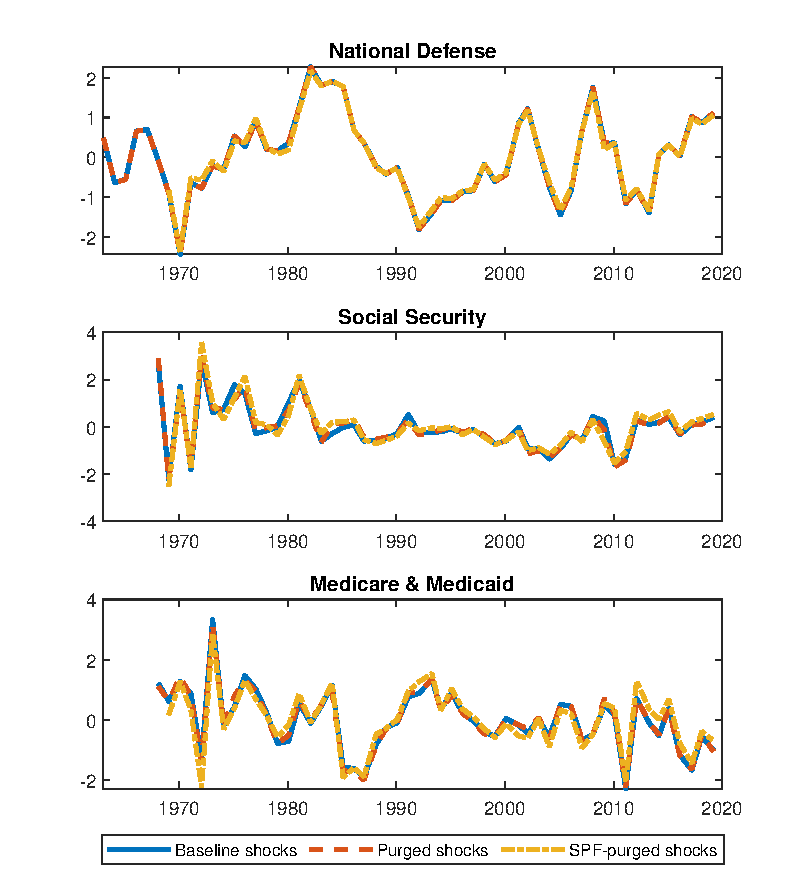
\includegraphics[trim=0mm 0mm 0mm 0mm,clip,width=0.7\textwidth]{figures and tables/shock_purged.pdf}
    \caption{\textbf{Baseline vs. purged measures of shocks.} 
    \\[0.5ex]
    \small
    The blue solid lines show the baseline measure of anticipated government spending shocks, constructed from the spending projections in U.S. budgets for each spending subcategory. The red dashed lines represent purged shocks obtained by regressing the baseline shocks on a constant and the expected growth rate of real GDP reported in the budgets. The yellow dash-dotted lines represent purged shocks obtained by regressing the baseline shocks on a constant, the expected growth rate of GDP, and the expected change in unemployment reported in the Survey of Professional Forecasters.}
    \label{fig:purged}
\end{figure}



\begin{figure}[t]
     \centering
     %\begin{subfigure}[b]{0.495\textwidth}
         \centering
        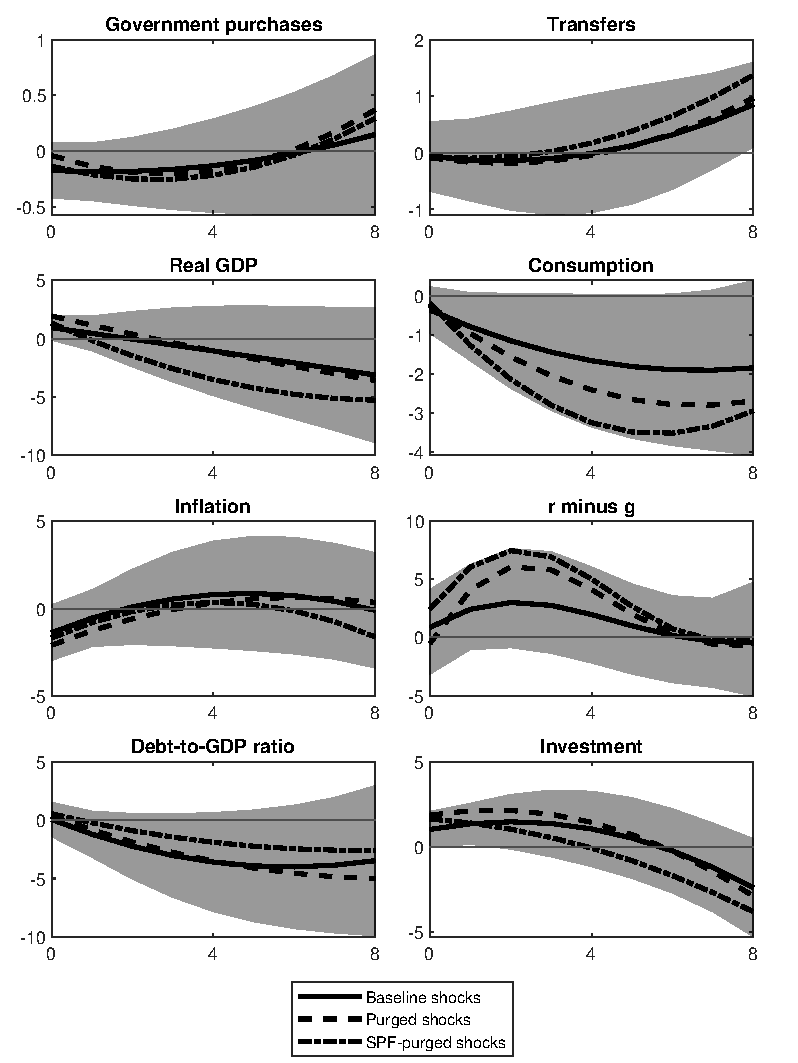
\includegraphics[trim=00mm 00mm 00mm 00mm, clip,width=1\textwidth]{figures and tables/figure_2_appD_MM_a.pdf}
         \caption{Anticip. shock to MM, linear}
    % \end{subfigure}
    % \hfill
     %\begin{subfigure}[b]{0.495\textwidth}
        % \centering
        % \includegraphics[trim=00mm 00mm 00mm 00mm, clip,width=1\textwidth]{figures and tables/figure_2_appD_MM_b.pdf}
        % \caption{Anticip. shock to MM, HISMI}
     %\end{subfigure}
    \caption{\textbf{Impulse responses to anticipated shocks to Medicare and Medicaid: Baseline vs. purged shocks.} 
    \\[0.5ex]
    \small
    Linear responses to an anticipated shock to Medicare \& Medicaid. 
    %Panel (b): state-dependent responses to an anticipated shock to Medicare \& Medicaid, conditioning on the periods of fiscal strain (red lines) or absence of fiscal strain (blue lines) in the HISMI funds.
    The solid lines show the responses to the baseline shocks, the dashed lines to the purged shocks, and the dash-dotted lines to the SPF-purged shocks.
    All responses are estimated over the sample 1968q1-2019q4. The set of controls always includes four lags of the shock, output, and transfers. Shaded areas: 90\% confidence bands for the baseline shocks.}
    \label{fig:IRF_purged_MM}
\end{figure}



\begin{figure}[t]
     \centering
     \begin{subfigure}[b]{0.495\textwidth}
        \centering
        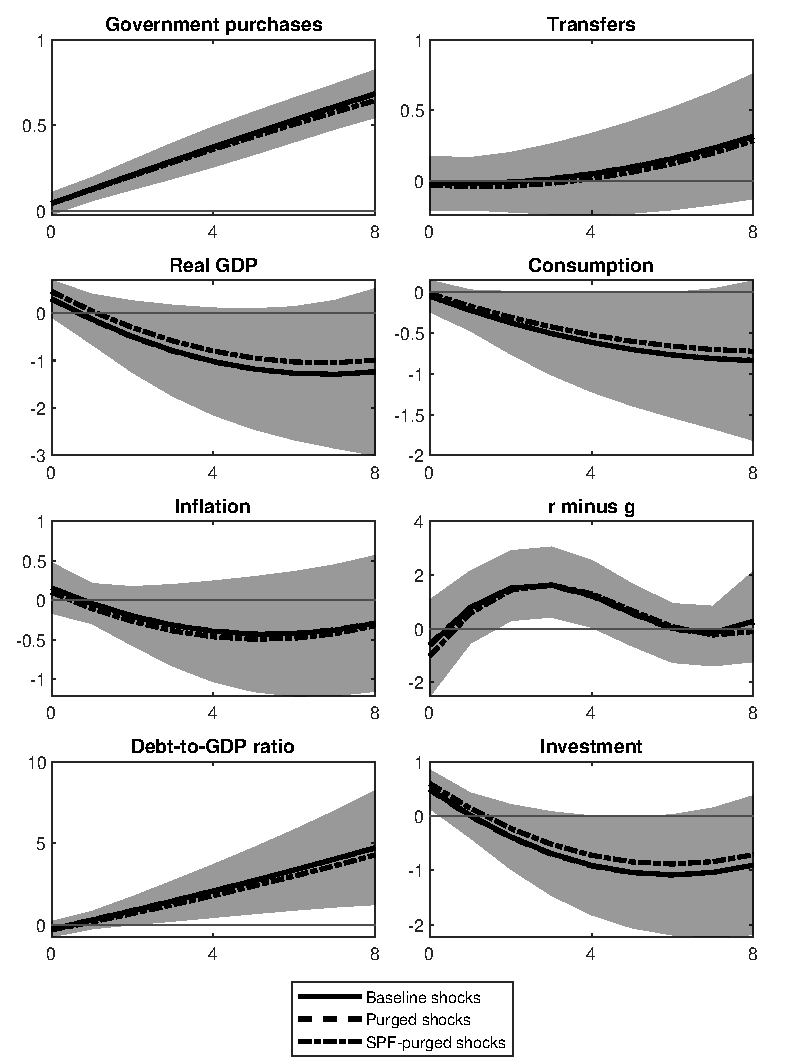
\includegraphics[trim=00mm 00mm 00mm 00mm, clip,width=1\textwidth]{figures and tables/figure_2_appD_ND_a.pdf}
        \caption{Anticip. shock to ND, linear}
     \end{subfigure}
     \hfill
     \begin{subfigure}[b]{0.495\textwidth}
        \centering
        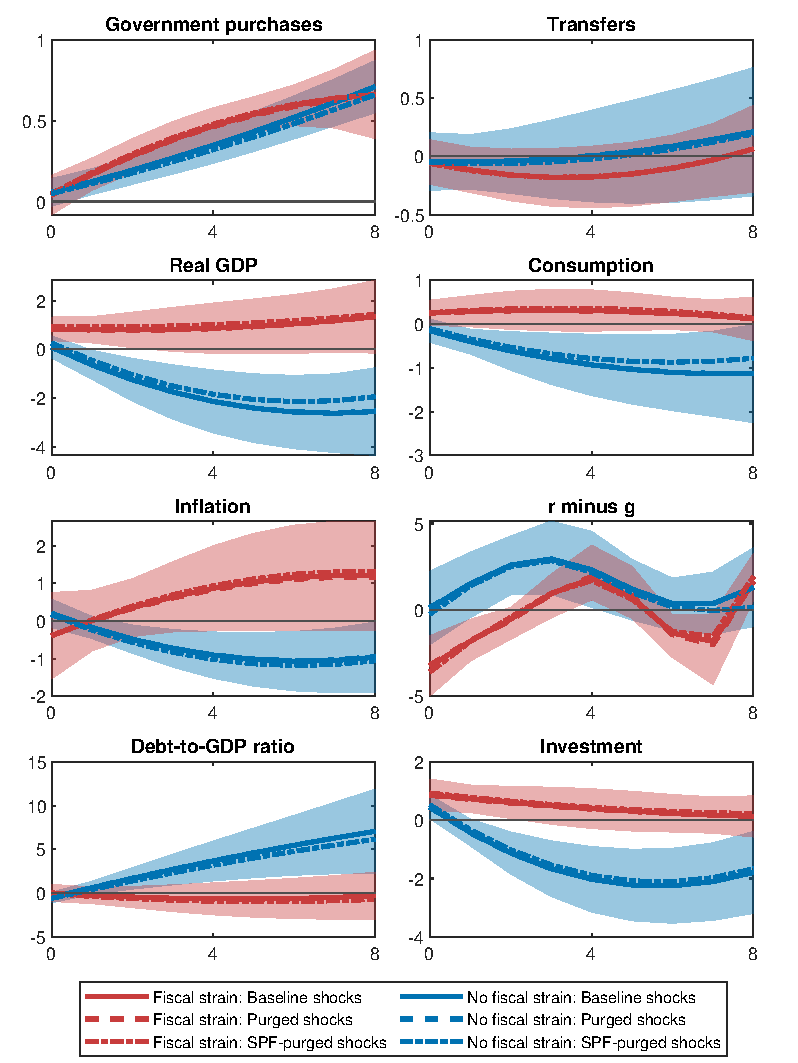
\includegraphics[trim=00mm 00mm 00mm 00mm, clip,width=1\textwidth]{figures and tables/figure_2_appD_ND_b.pdf}
        \caption{Anticip. shock to ND, FI}
     \end{subfigure}
    \caption{\textbf{Impulse responses to anticipated shocks to National Defense: Baseline vs. purged shocks.} 
    \\[0.5ex]
    \small
    Panel (a): linear responses to an anticipated shock to National Defense. Panel (b): state-dependent responses to an anticipated shock to National Defense, conditioning on the periods of fiscal strain (red lines) or absence of fiscal strain (blue lines) in the Fiscal index.
    In all panels, the solid lines show the responses to the baseline shocks, the dashed lines to the purged shocks, and the dash-dotted lines to the SPF-purged shocks.
    All responses are estimated over the sample 1968q1-2019q4. The set of controls always includes four lags of the shock, output, and government purchases. Shaded areas: 90\% confidence bands for the baseline shocks.}
    \label{fig:IRF_purged_ND}
\end{figure}

\begin{figure}[t]
     \centering
     \begin{subfigure}[b]{0.495\textwidth}
         \centering
        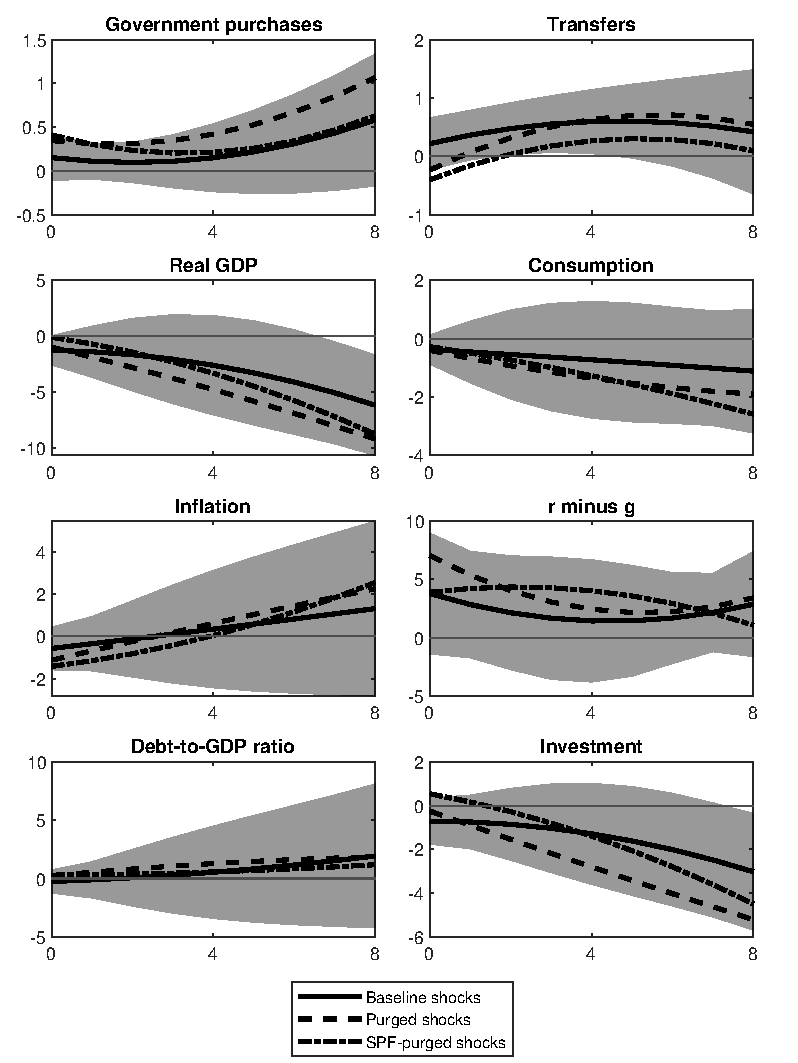
\includegraphics[trim=00mm 00mm 00mm 00mm, clip,width=1\textwidth]{figures and tables/figure_2_appD_SS_a.pdf}
         \caption{Anticip. shock to SS, linear}
     \end{subfigure}
     \hfill
     \begin{subfigure}[b]{0.495\textwidth}
         \centering
         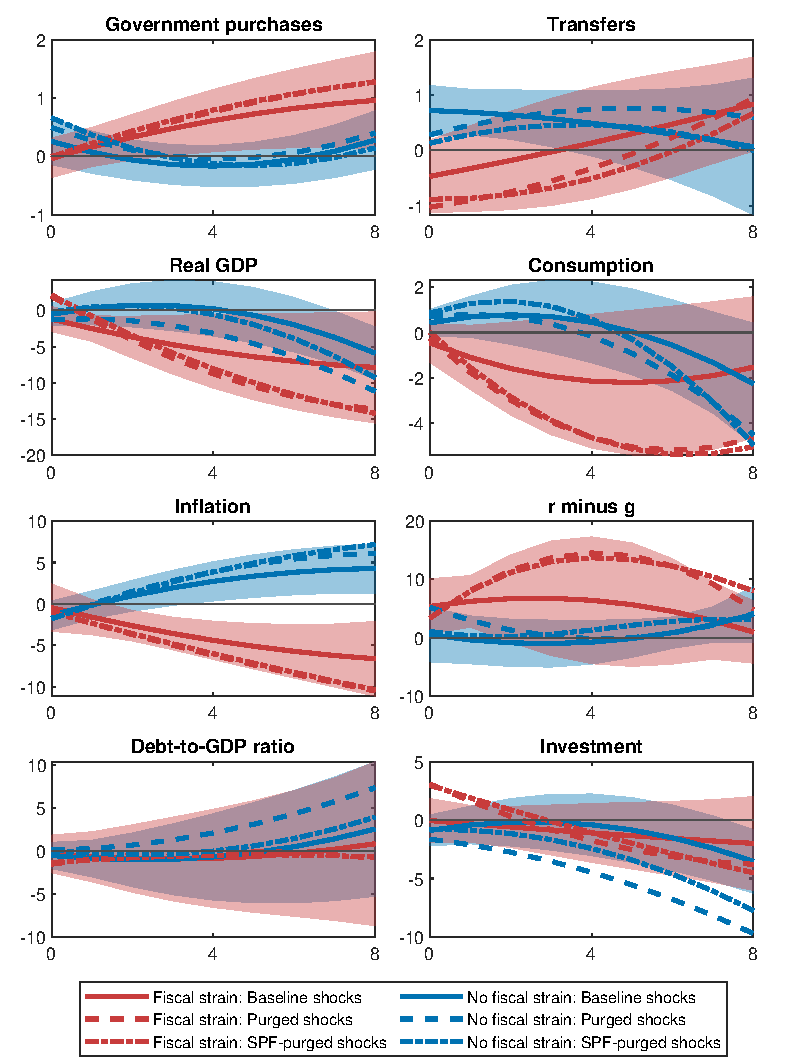
\includegraphics[trim=00mm 00mm 00mm 00mm, clip,width=1\textwidth]{figures and tables/figure_2_appD_SS_b.pdf}
         \caption{Anticip. shock to SS, OASDI}
     \end{subfigure}
    \caption{\textbf{Impulse responses to anticipated shocks to Social Security: Baseline vs. purged shocks.} 
    \\[0.5ex]
    \small
    Panel (a): linear responses to an anticipated shock to Social Security. Panel (b): state-dependent responses to an anticipated shock to Social Security, conditioning on the periods of fiscal strain (red lines) or absence of fiscal strain (blue lines) in the OASDI funds.
    In all panels, the solid lines show the responses to the baseline shocks, the dashed lines to the purged shocks, and the dash-dotted lines to the SPF-purged shocks.
    All responses are estimated over the sample 1968q1-2019q4. The set of controls always includes four lags of the shock, output, and transfers. Shaded areas: 90\% confidence bands for the baseline shocks.}
    \label{fig:IRF_purged_SS}
\end{figure}

\FloatBarrier
\newpage
\section{Supplementary Figures}\label{app:sec:suppl}

\begin{figure}[h] 
    \centering
    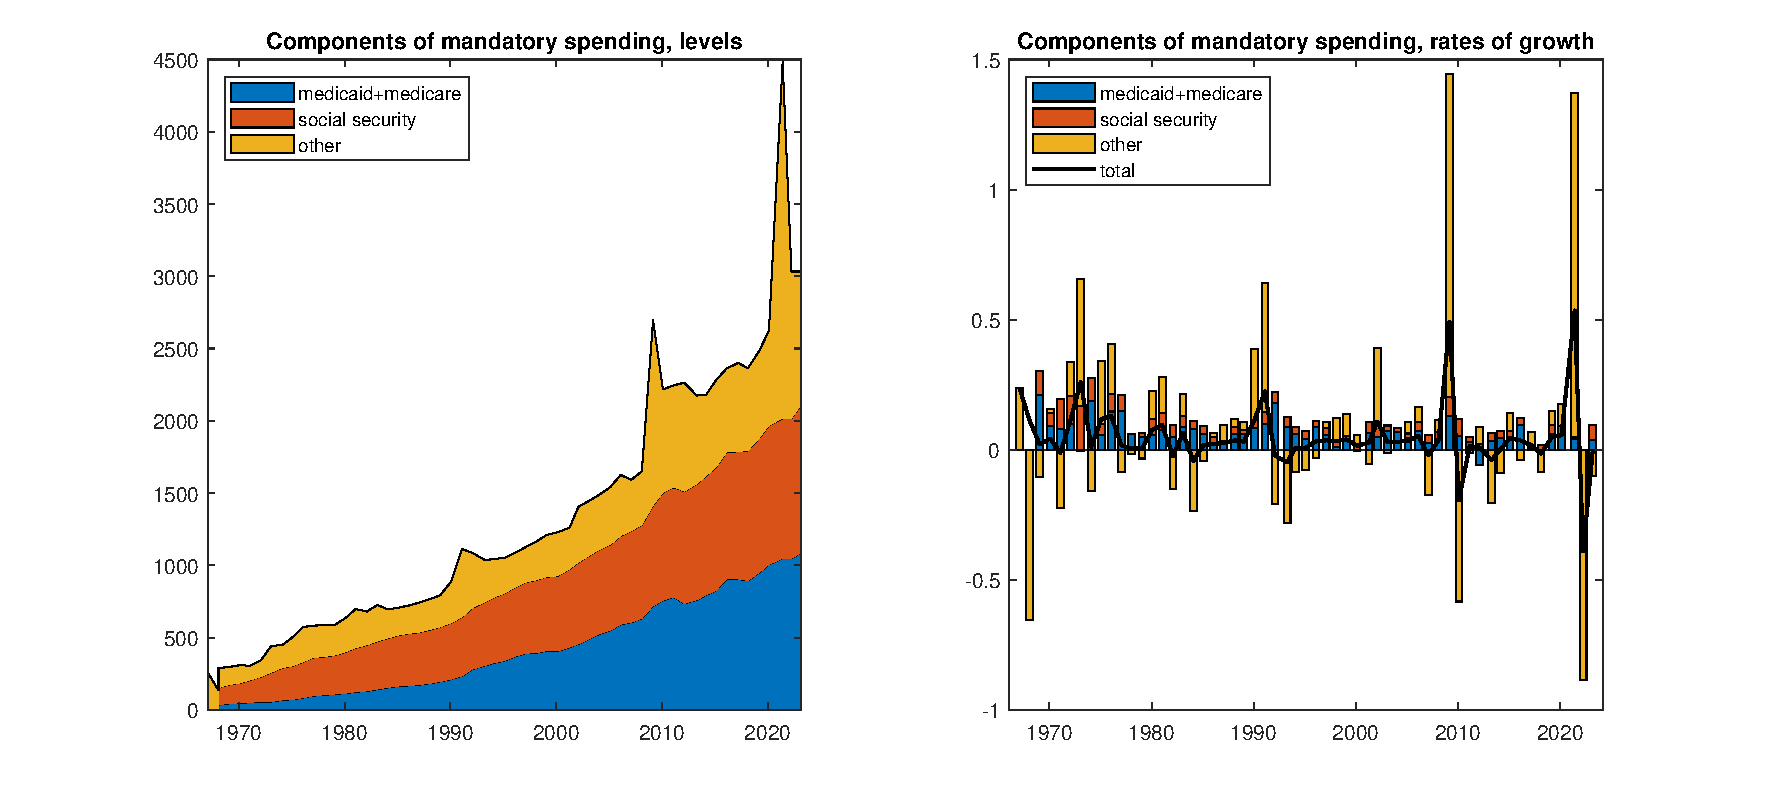
\includegraphics[trim=25mm 5mm 25mm 5mm,clip,width=0.9\textwidth]{figures and tables/figure_mandatory.pdf}
\end{figure}

\begin{figure}[h]
    \centering
    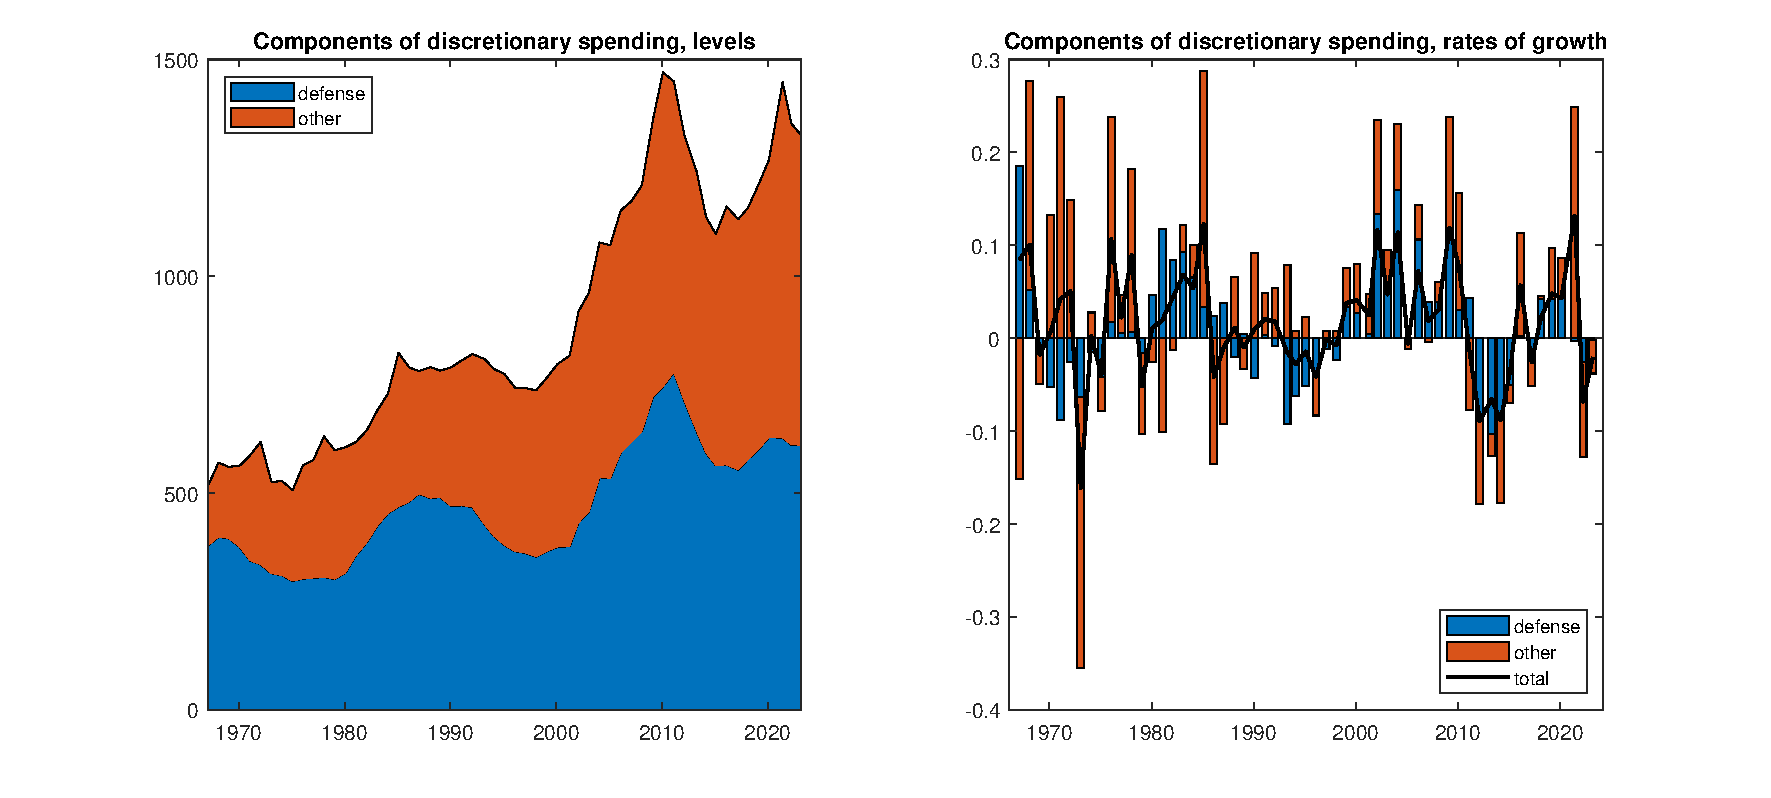
\includegraphics[trim=25mm 5mm 25mm 5mm,clip,width=0.9\textwidth]{figures and tables/figure_discretionary.pdf}
\end{figure}

% 
\begin{table}[h!]
\centering
\caption{Historical debt ceiling levels}  \label{table:debt_ceiling}
\begin{tabular}{|>{\raggedright}p{5cm}|>{\raggedleft\arraybackslash}p{5cm}|>{\raggedleft\arraybackslash}p{3cm}|}
\hline
\textbf{Date} & \textbf{Debt Ceiling} & \textbf{Change in Debt Ceiling} \\
\hline
August 5, 1997        & 5,95     & 450  \\
June 11, 2002         & 6,4      & 450  \\
May 27, 2003          & 7,384    & 984  \\
November 16, 2004     & 8,184    & 800  \\
March 20, 2006        & 8,965    & 781  \\
September 29, 2007    & 9,815    & 850  \\
June 5, 2008          & 10,615   & 800  \\
October 3, 2008       & 11,315   & 700  \\
February 17, 2009     & 12,104   & 789  \\
December 24, 2009     & 12,394   & 290  \\
February 12, 2010     & 14,294   & 1,900 \\
January 30, 2012      & 16,394   & 2,100 \\
February 4, 2013      & Suspended & -   \\
May 19, 2013          & 16,699   & 305  \\
October 17, 2013      & Suspended & -   \\
February 7, 2014      & 17,212   & 213  \\
March 15, 2015        & 18,113   & 901  \\
October 30, 2015      & Suspended & -   \\
March 15, 2017        & 19,847 (de facto) & 1,734 \\
September 30, 2017    & Suspended & -   \\
March 1, 2019         & 22,030 (de facto) & 2,183 \\
August 2, 2019        & Suspended & -   \\
July 31, 2021         & 28,500 (de facto) & 6,470 \\
October 14, 2021      & 28,9     & 400  \\
December 16, 2021     & 31,4     & 2,500 \\
\hline
\end{tabular}
\end{table}


\begin{figure}[h]
    \centering
    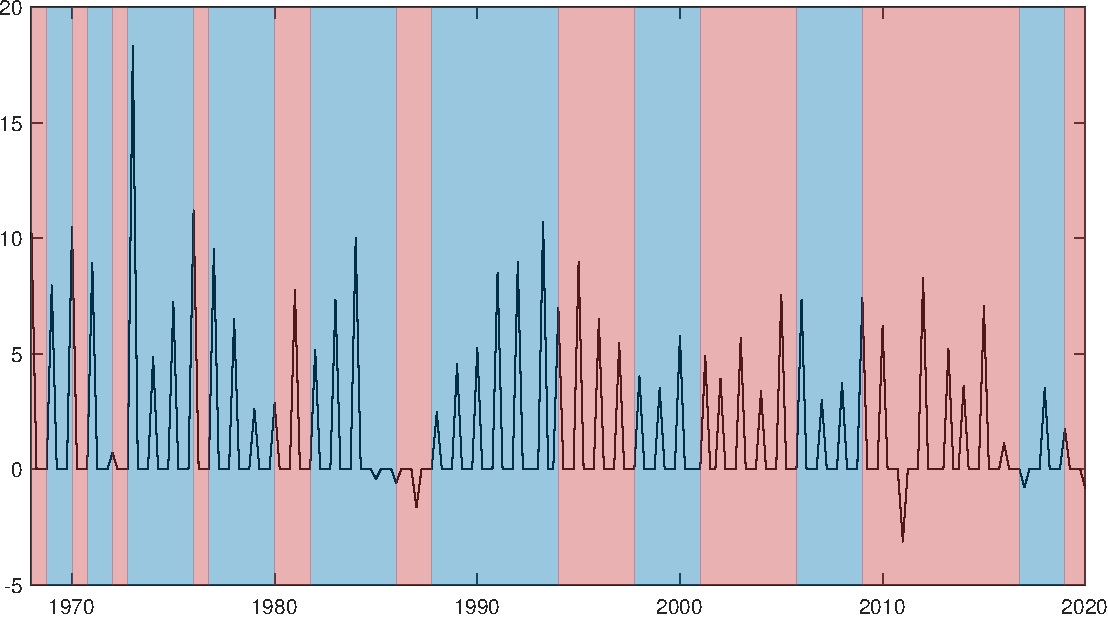
\includegraphics[trim=00mm 00mm 00mm 00mm, clip, scale=0.5]{figures and tables/f1q_state_HISMI.pdf}
\caption{\textbf{Anticipated shocks to Medicare \& Medicaid and fiscal capacity based on the HISMI funds.}
\\[0.5ex]
\small
Black line: time series of anticipated shocks to Medicare \& Medicaid, in percentage points. 
Shaded areas: periods of fiscal strain (red) or absence of fiscal strain (blue) in the HISMI funds.}
\end{figure}

\begin{figure}[h]
    \centering
    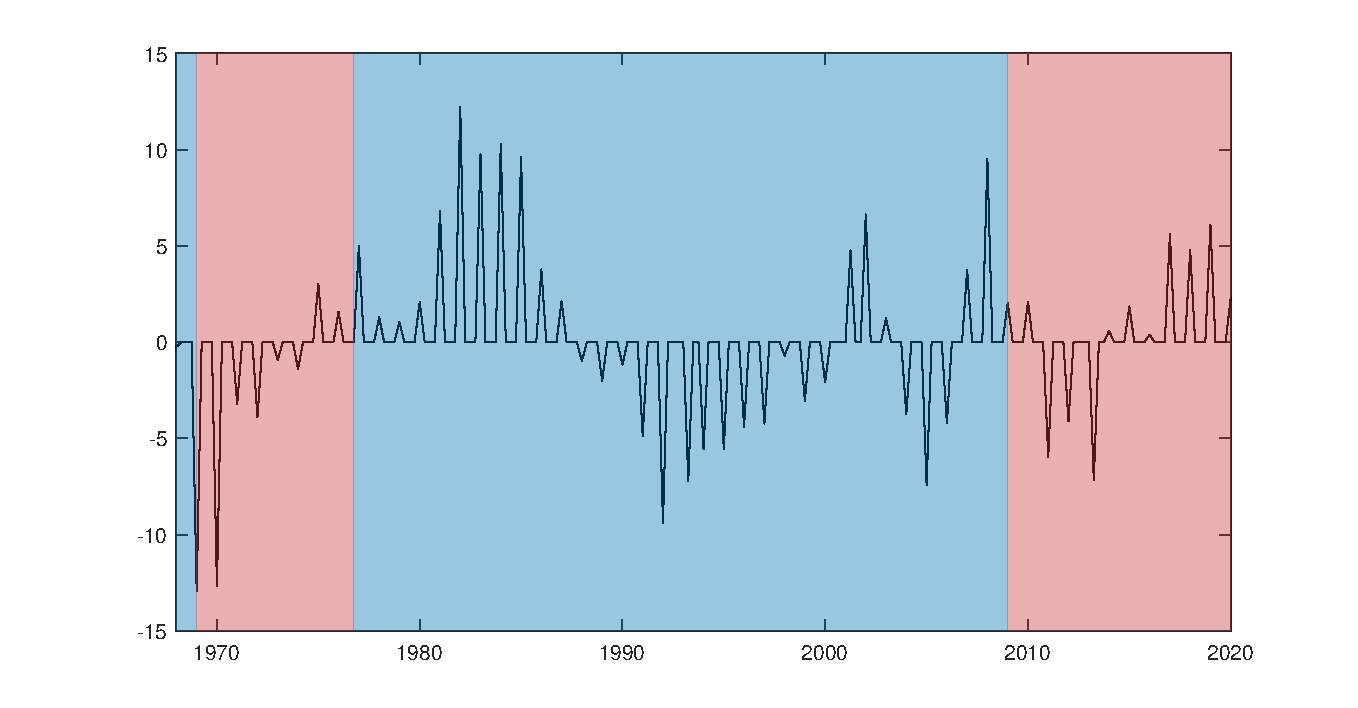
\includegraphics[trim=00mm 00mm 00mm 00mm, clip, scale=0.5]{figures and tables/f1q_state_fiscalindexdoppio.pdf}
\caption{\textbf{Anticipated shocks to National Defense and fiscal capacity based on the Fiscal index.}
\\[0.5ex]
\small
Black line: time series of anticipated shocks to National Defense, in percentage points. 
Shaded areas: periods of fiscal strain (red) or absence of fiscal strain (blue) in the Fiscal index.}
\end{figure}
% \begin{figure}[t!]
%     \centering
%     \includegraphics[scale=0.8]{figures and tables/unfunded tr.PNG}
%     \caption{Unfunded transfers}
%     \label{fig:unfunded tr}
% \end{figure}

\FloatBarrier
\newpage
\section{Trustees Reports and the Evolution of Actuarial Assessments, 1969–1976}\label{app:sec:supplem}
\subsection*{Old-Age, Survivors, and Disability Insurance (OASDI)}
This Section documents the evolution of official actuarial assessments of the Old-Age, Survivors, and Disability Insurance (OASDI) system as reported in the Trustees Reports from 1969 to 1976. The sequence of Tables (see Figure TOT) illustrates a sharp break in the interpretation of actuarial balance and trust fund solvency beginning in 1974.
Under the legislation in force in the late 1960s, most importantly the 1967 Amendments, projected benefit costs stabilized as a share of taxable payroll, while scheduled payroll tax rates exceeded long-run actuarial cost rates. Favorable demographic and macroeconomic conditions, including relatively stable mortality projections, supported this assessment.

\paragraph{1969–1971: Positive Actuarial Balances.}
The 1969 Trustees Report presents long-range actuarial balance estimates under low-cost, intermediate-cost, and high-cost assumptions (1969 Report, p.~37). Under both the low-cost and intermediate-cost scenarios, the total OASDI actuarial balance is clearly positive (1.14\% and 0.53\% of taxable payroll, respectively). Even under the high-cost scenario, the reported deficit is modest (-0.17\%).

Similarly, the 1970 Trustees Report continues to report actuarial balances close to zero. Under the intermediate-cost assumptions, the total actuarial balance is -0.08\% of taxable payroll, while the low-cost scenario yields a surplus of +0.54\%. The 1971 Trustees Report shows a comparable pattern: a small surplus under low-cost assumptions (+0.58\%) and a near-zero balance under intermediate-cost assumptions (-0.10\%).
Across these reports, two features stand out. First, actuarial balance estimates are clustered tightly around zero, indicating no perceived structural financing gap. Second, rather than framing projections in terms of binding solvency constraints or trust fund exhaustion, pre-1974 Trustees Reports present a range of alternative cost scenarios, treating actuarial balance as a sensitivity measure rather than as an indicator of impending insolvency.
\paragraph{1972–1973: Apparent Actuarial Stability.}
The 1972 Trustees Report presents actuarial balance estimates under both level-earnings assumptions (Table 17) and dynamic assumptions (Table 19). Under level-earnings assumptions, the total actuarial balance is essentially zero (+0.05\%). Under dynamic assumptions, which incorporate rising nominal earnings and automatic benefit increases, the actuarial balance is reported as strongly positive (+1.04\%).
The 1973 Trustees Report, using dynamic assumptions, shows a modest deterioration but still no indication of severe imbalance. The total actuarial balance is reported as -0.32\% of taxable payroll. While negative, this value remains small in magnitude and is not framed as implying imminent trust fund exhaustion or the need for corrective legislation.
Taken together, the 1972 and 1973 reports reinforce the prevailing perception that OASDI remained broadly actuarially sound under current law, even after the introduction of automatic cost-of-living adjustments. Dynamic assumptions were interpreted as benign, and automatic indexation was not yet viewed as a source of systemic risk.

\paragraph{1974: A Downward Revision in Actuarial Balance.}
The 1974 Trustees Report marks a clear break with earlier assessments. Table~20 reports a total actuarial balance of -2.98\% of taxable payroll over the 75-year horizon (1974--2048) under dynamic assumptions. This represents an order-of-magnitude deterioration relative to earlier reports. This shift is driven by a sharp upward revision in the projected average cost of the system (13.89\% of taxable payroll) relative to the average rate in the present tax schedule (10.91\%). Unlike earlier reports, the 1974 assessment explicitly attributes this deterioration to revised demographic projections and to the interaction of high inflation with the automatic benefit indexation provisions enacted in 1972, including the benefit formula error later corrected in the 1977 amendments.

Importantly, the presentation now centers on long-run imbalance and implicitly on trust fund exhaustion. Actuarial balance is no longer treated as a near-zero accounting residual but as a measure of the permanent contribution increase or benefit reduction required to restore solvency.

\paragraph{1975–1976: Consolidation of the Insolvency Narrative.}

The 1975 Trustees Report shifts presentation from actuarial balance tables to explicit comparisons of expenditures and tax rates over successive 25-year periods (Table 21). Over the full 75-year horizon, the report shows a total actuarial deficit of -5.32\% of taxable payroll, substantially larger than the already-negative 1974 estimate. Deficits widen dramatically in later subperiods, underscoring the long-run nature of the imbalance. This reassessment was reinforced by contemporaneous external reviews commissioned by Congress, most notably the 1975 Report of the Consultant Panel on Social Security chaired by \cite{Hsiao1975Report}, which independently validated the Trustees’ diagnosis and emphasized that earlier projections had been overly optimistic.
The 1976 Trustees Report confirms this perspective under alternative intermediate assumptions (Table 27). The total 75-year difference between expenditures and taxes is reported as -7.96\% of taxable payroll, with particularly large shortfalls in the final 25-year period. The convergence between the Trustees Reports and the conclusions of the Hsiao Panel eliminated remaining ambiguity about the long-run outlook of OASDI financing. By this point, the Trustees Reports consistently frame OASDI financing in terms of persistent actuarial deficits and the inevitability of future corrective action.
The sequence of Trustees Reports from 1969 to 1976 documents a clear regime shift in the interpretation of OASDI financing. Prior to 1974, actuarial balance estimates clustered around zero and were presented as evidence of long-run sustainability. Automatic indexation and dynamic earnings growth were viewed as compatible with actuarial soundness, and no expectation of future policy adjustment was embedded in official projections.
Beginning in 1974, revised assumptions and the realization of sustained high inflation transformed this narrative. Actuarial balance became sharply negative, trust fund exhaustion emerged as a central organizing concept, and future tax increases or benefit reductions became an implicit component of the financing outlook. This shift in the actuarial narrative fundamentally altered expectations about fiscal backing and the role of the OASDI trust funds within the federal budget.
\paragraph{Legislative response}
The new outlook shaped subsequent legislation. The Social Security Amendments of 1977 and the crisis-driven reforms of 1983 raised payroll taxes, reduced benefit generosity, increased the retirement age, and expanded the contributory base. The reassessment also changed how earlier expansions were understood: prior to 1974, legislative expansions and the introduction of automatic indexation had effectively converted the program into a “retirement wage,” with benefits designed to substitute for labor income and maintain living standards after retirement (Myles, 1988).

\subsection*{Medical Hospital Insurace (HI)}

This section documents the evolution of actuarial assessments for the Medicare Hospital Insurance (HI) trust fund as reported in the Trustees Reports from 1969 to 1976. In contrast to OASDI, these reports reveal no regime shift in the interpretation of actuarial soundness. From the earliest assessments in the late 1960s, HI is consistently portrayed as subject to actuarial pressure, with projected costs closely tracking or exceeding scheduled contribution rates and trust fund balances described as finite and vulnerable to depletion. The 1969 Trustees Report, for instance, presents detailed projections of annual cash flows, interest earnings, and trust fund balances under intermediate-cost assumptions (Table~5), explicitly anticipating fund exhaustion within the projection horizon. Subsequent reports for 1970 and 1971 reinforce this view, with alternative assumptions for the earnings base (Tables~5a and~5b in the 1970 report and Table~5 in the 1971 report) continuing to project depletion rather than permanent surplus accumulation.

Beginning in 1972, the Trustees Reports introduce explicit actuarial balance calculations for HI. The 1972 report documents a negative actuarial balance over the 25-year horizon 1972--1996 (Table~9), reflecting an average cost rate exceeding the scheduled contribution rate, while the 1973 report reports a similarly small but still negative actuarial balance over 1973--1997 (Table~8). These near-zero balances are not framed as evidence of overfinancing or long-run sustainability, but rather as indicative of short- to medium-run imbalance. In 1974, actuarial balance turns marginally positive over the 1974--1998 horizon (Table~9), yet the accompanying discussion explicitly characterizes this outcome as conditional and short-horizon, without altering long-run expectations. The 1975 report returns to a negative actuarial balance over 1975--1999, again emphasizing the fragility of HI financing in the face of medical cost growth.

The 1976 Trustees Report further underscores the persistence of actuarial stress. Under intermediate assumptions, actuarial balance remains negative over the 1976--2000 horizon (Table~9), while alternative assumption sets explored in Table~11 generate a wide range of outcomes, from modest surpluses to sizable deficits. This sensitivity to assumptions reinforces the Trustees’ long-standing emphasis on uncertainty and on the likelihood of future financing adjustments. Taken together, the Trustees Reports from 1969 to 1976 portray Medicare Hospital Insurance as a program under persistent actuarial pressure from its inception. Unlike OASDI, HI is never described as actuarially overfunded or as generating long-run surpluses; trust fund depletion is routinely projected, and actuarial balance fluctuates around zero without anchoring expectations of permanent solvency. As a result, expectations of future policy adjustment are embedded in the HI financing framework from the outset. Persistent actuarial imbalance is thus a defining feature of HI rather than a regime shift, shaping expectations of fiscal backing and adjustment continuously over time.

\FloatBarrier
%\newpage
\section{Social Security: model equations and solution}
\label{sec:app:model}
This appendix describes the model and solution method used in Section~\ref{sec:model}. Date $k=0$ is the announcement date; subsequent paths are deterministic. The actuarial horizon is $K$, and $K^*$ is the first projected reserve-floor breach. Fiscal stocks and flows are in units of fixed reference output, normalized to $\bar Y=100$ in the illustration. A superscript $0$ denotes the no-news reference path and $\Delta$ denotes a deviation from it.

\subsection{Households and firms}
The representative household has unit mass and an elderly share $\omega_k$. Each young member supplies $n_k$ hours, giving aggregate labor $N_k=(1-\omega_k)n_k$. Members pool consumption, earnings, taxes, transfers, and assets. Preferences are
\begin{equation}
 \sum_{k=0}^{\infty}\beta^k
 \left[\frac{C_k^{1-\sigma}}{1-\sigma}
 -\chi\frac{n_k^{1+\nu}}{1+\nu}\right],
 \qquad 0<\beta<1,\quad \sigma,\chi>0,\quad\nu\geq0,
 \label{eq:ga_preferences}
\end{equation}
with log utility when $\sigma=1$. Let $W_k$ denote the nominal wage, $D_k$ nominal profits, and $i_k$ the gross nominal return from $k$ to $k+1$. The household budget is
\begin{equation}
 \begin{split}
 P_kC_k+B_k^{ON}={}&W_k(1-\omega_k)n_k+D_k
 +i_{k-1}B_{k-1}^{ON}\\
 &-P_k(\bar s^{ON}+\tau_k+a_k).
 \end{split}
 \label{eq:ga_hh_budget}
\end{equation}
Here $\bar s^{ON}$ is lump-sum taxation outside Social Security, $\tau_k$ is the current-law Social Security surplus, and $a_k\geq0$ is a lump-sum correction. With contributions $\bar p^Y$ per young member and benefits $\bar v^O$ per old member,
\begin{equation}
 \tau_k=(1-\omega_k)\bar p^Y-\omega_k\bar v^O,
 \qquad s_k^{OFF}=\tau_k+a_k.
 \label{eq:ga_ss_balance}
\end{equation}
The correction can be implemented as an extra contribution $a_k/(1-\omega_k)$ per young member or an equivalent aggregate benefit reduction.

A competitive final-good sector aggregates varieties with elasticity $\epsilon_p>1$. Intermediate firms produce $Y_k(j)=A_kN_k(j)$ and reset prices with probability $1-\theta$. Set $A_k=\bar A/(1-\omega_k)$. The labor condition and real marginal cost are
\begin{equation}
 \frac{W_k}{P_k}(1-\omega_k)=\chi n_k^\nu C_k^\sigma,
 \qquad mc_k=\frac{W_k}{P_kA_k}
 =\frac{\chi n_k^\nu C_k^\sigma}{\bar A}.
 \label{eq:ga_mc}
\end{equation}
There are no government purchases, so $C_k=Y_k$. Around zero inflation, price dispersion is second order and $Y_k=\bar A n_k$ to first order. The productivity offset and the absence of a demographic weight on labor disutility keep natural output constant. The Euler equation and Calvo pricing therefore give \eqref{eq:ga_nk}, with
\begin{equation}
 \kappa=\frac{(1-\theta)(1-\beta\theta)}{\theta}(\sigma+\nu),
 \qquad r=\beta^{-1}.
 \label{eq:ga_kappa}
\end{equation}
The household discount factor is
\begin{equation}
 q_k=\beta^k\left(\frac{C_k}{C_0}\right)^{-\sigma}
 =\beta^k e^{\sigma(y_0-y_k)}
 \simeq\beta^k[1+\sigma(y_0-y_k)].
 \label{eq:ga_sdf}
\end{equation}

\subsection{Fiscal accounts and the reserve rule}
Gross Treasury debt is $B_k=B_k^{ON}+B_k^{OFF}$. The Treasury and trust-fund budgets are
\begin{equation}
 B_k=i_{k-1}B_{k-1}-P_k\bar s^{ON},
 \qquad B_k^{OFF}=i_{k-1}B_{k-1}^{OFF}+P_k(\tau_k+a_k).
 \label{eq:ga_nominal_budgets}
\end{equation}
Trust-fund securities cancel on consolidation. Subtraction yields the public-debt budget in \eqref{eq:ga_public_debt}, with $b_k^j=B_k^j/P_k$ and $R_k=i_{k-1}P_{k-1}/P_k$. The non-Social-Security surplus $\bar s^{ON}$ is fixed within each experiment, while the trust fund cannot borrow. Household transversality, $\lim_{T\to\infty}q_Tb_T^{ON}=0$, gives the valuation condition \eqref{eq:ga_valuation}; no separate zero-terminal-value condition is imposed on internal trust-fund assets.

News revises $\omega_k$ and $\tau_k$ for $1\leq k\leq K$, leaving $\tau_0$ unchanged; $\omega_k=\omega_K$ and $\tau_k=\tau_K$ for $k>K$. The uncorrected reserve projection and first breach date satisfy
\begin{align}
 \widetilde b_0^{OFF}&=R_0b_{-1}^{OFF}+\tau_0,
 &\widetilde b_k^{OFF}&=R_k\widetilde b_{k-1}^{OFF}+\tau_k,
 \quad k\geq1,\nonumber\\*
 K^*&=\inf\{k\geq1:\widetilde b_k^{OFF}<\underline b\},
 &\inf\varnothing&=\infty.
 \label{eq:ga_projection}
\end{align}
For finite $K^*\leq K$, targets are computed backward:
\begin{equation}
 m_K=\underline b,\qquad
 m_k=\max\left\{\underline b,
 \frac{m_{k+1}-\tau_{k+1}}{R_{k+1}}\right\},
 \quad k=K-1,\ldots,K^*.
 \label{eq:ga_targets}
\end{equation}
Set $m_k=\underline b$ for $k>K$. If $K<K^*<\infty$, intervention starts at $K^*$ with target $\underline b$ and no backward recursion. Given these targets, use \eqref{eq:ga_adjustment} with
\begin{equation}
 b_k^{pre}=R_kb_{k-1}^{OFF}+\tau_k,
 \qquad b_k^{OFF}=b_k^{pre}+a_k.
 \label{eq:ga_actual_reserves}
\end{equation}
There is no correction before $K^*$, including at date 0. Thereafter, $b_k^{OFF}\geq m_k\geq\underline b$. The rule prescribes no easing when reserves exceed the target, and corrections can continue beyond $K$. The entire schedule is anticipated at the announcement.

\subsection{No-news reference paths}
For each scenario, set $\pi_k^0=y_k^0=0$ and $R_k^0=r$, and apply the reserve rule to the current-law path $\tau_k^0$, obtaining $a_k^0$ and $b_k^{OFF,0}$. Define
\begin{equation}
 V^0=rb_{-1}^{ON},\qquad
 s_k^0=\bar s^{ON}+\tau_k^0+a_k^0.
 \label{eq:ga_reference_surplus}
\end{equation}
The constant outside surplus is chosen to satisfy the reference valuation condition:
\begin{equation}
 \bar s^{ON}=(1-\beta)\left[
 V^0-\sum_{k=0}^{\infty}\beta^k(\tau_k^0+a_k^0)\right].
 \label{eq:ga_reference}
\end{equation}
It is held fixed after the news. This normalization is performed separately for each scenario, and the depletion reference already includes anticipated corrections. Reserves need not be stationary along the no-news path.

The illustration uses $(\beta,\sigma,\nu,\theta,\phi)=(0.96,1,1,0.6,0.5)$, $b_{-1}^{ON}=60$, $b_{-1}^{OFF}=10.6$, and $\underline b=8$. The reference balances are $\tau_k^0=0.6$ and $-0.7$; the corresponding outside surpluses are $1.9$ and $2.941667$. News sets $\Delta\tau_k=-0.015\min\{k,K\}$ with $K=10$, so the terminal deterioration persists indefinitely.

\subsection{Numerical solution}
The solution combines a first-order New Keynesian and fiscal-accounting system with the reserve threshold and positive-part correction rule. It is computed by a scalar search over impact inflation, with the fiscal path recalculated at each trial.

\paragraph{1. Bounded private-sector path.}
Substituting $\pi_{k+1}=\rho\pi_k$ into \eqref{eq:ga_nk} gives the stable root
\begin{equation}
 \sigma(1-\rho)(1-\beta\rho)=\kappa(\rho-\phi),
 \qquad \phi<\rho<1.
 \label{eq:ga_root}
\end{equation}
For a trial $\pi_0$, discard the explosive root and compute
\begin{equation}
 \pi_k=\rho^k\pi_0,\qquad
 y_k=\frac{1-\beta\rho}{\kappa}\rho^k\pi_0,
 \qquad\widehat i_k=\phi\pi_k.
 \label{eq:ga_bounded_path}
\end{equation}

\paragraph{2. Reserve revaluation and correction.}
Because the inherited nominal rate is predetermined, the log real-return deviations are
\begin{equation}
 \widehat R_0=-\pi_0,\qquad
 \widehat R_k=\widehat i_{k-1}-\pi_k
 =\sigma(y_k-y_{k-1}),\quad k\geq1.
 \label{eq:ga_real_returns}
\end{equation}
Set $R_k\simeq r(1+\widehat R_k)$ and define $\mathcal R_k=r b_{k-1}^{OFF,0}\widehat R_k$. The first-order reserve-accounting equation is
\begin{equation}
 \Delta b_k^{OFF}=r\Delta b_{k-1}^{OFF}
 +\Delta\tau_k+\Delta a_k+\mathcal R_k,
 \qquad \Delta b_{-1}^{OFF}=0,
 \label{eq:ga_reserve_linear}
\end{equation}
where $\Delta a_k=a_k-a_k^0$ and $\mathcal R_0=-r b_{-1}^{OFF}\pi_0$. Products of deviations are omitted.

To select the breach date, the implementation suppresses corrections and iterates $\widetilde b_k^{OFF}=r\widetilde b_{k-1}^{OFF}+\tau_k+\mathcal R_k$, starting from $b_{-1}^{OFF}$. Revaluation is evaluated at the reference stocks $b_{k-1}^{OFF,0}$, including any reference correction. After selecting $K^*$, compute \eqref{eq:ga_targets} using the trial returns. Then apply \eqref{eq:ga_adjustment} with $b_k^{pre}=r b_{k-1}^{OFF}+\tau_k+\mathcal R_k$ and update reserves through \eqref{eq:ga_reserve_linear}. The target ratios and positive-part operators are retained; the procedure is not a global nonlinear solution.

\paragraph{3. Fiscal valuation.}
Since $\bar s^{ON}$ is unchanged, the consolidated surplus revision is $\Delta s_k=\Delta\tau_k+\Delta a_k$. Expand \eqref{eq:ga_valuation} around the reference path, using \eqref{eq:ga_sdf} and $i_{-1}B_{-1}^{ON}/P_0=V^0e^{-\pi_0}$. The first-order valuation residual, truncated at numerical horizon $H$, is
\begin{equation}
 F_H(\pi_0)=V^0\pi_0+
 \sum_{k=0}^{H}\beta^k
 \left[\Delta\tau_k+\Delta a_k+s_k^0\sigma(y_0-y_k)\right].
 \label{eq:ga_numerical_root}
\end{equation}
The last term captures changes in household discounting. Products of deviations in surpluses and discount factors are second order. Brent's method searches over $\pi_0\in[-0.10,0.10]$ for $F_H(\pi_0)=0$, repeating steps 1--2 at every trial. We use $H=800$ in both valuation and reference calibration; it approximates the infinite continuation and is distinct from the actuarial horizon $K=10$.

The computed solution is checked against the IS and Phillips curves, reserve accounting, and fiscal valuation, with $|F_H|<10^{-9}$. Reserves must remain positive, and the projected intervention date is checked at $\pi_0\pm10^{-6}$ to verify that the solution lies locally on the same branch of the correction rule.
\end{document}





